\documentclass[icelandic,]{book}
\usepackage{lmodern}
\usepackage{amssymb,amsmath}
\usepackage{ifxetex,ifluatex}
\usepackage{fixltx2e} % provides \textsubscript
\ifnum 0\ifxetex 1\fi\ifluatex 1\fi=0 % if pdftex
  \usepackage[T1]{fontenc}
  \usepackage[utf8]{inputenc}
\else % if luatex or xelatex
  \ifxetex
    \usepackage{mathspec}
  \else
    \usepackage{fontspec}
  \fi
  \defaultfontfeatures{Ligatures=TeX,Scale=MatchLowercase}
\fi
% use upquote if available, for straight quotes in verbatim environments
\IfFileExists{upquote.sty}{\usepackage{upquote}}{}
% use microtype if available
\IfFileExists{microtype.sty}{%
\usepackage{microtype}
\UseMicrotypeSet[protrusion]{basicmath} % disable protrusion for tt fonts
}{}
\usepackage{hyperref}
\hypersetup{unicode=true,
            pdftitle={Örplast í hafinu við Ísland},
            pdfborder={0 0 0},
            breaklinks=true}
\urlstyle{same}  % don't use monospace font for urls
\ifnum 0\ifxetex 1\fi\ifluatex 1\fi=0 % if pdftex
  \usepackage[shorthands=off,main=icelandic]{babel}
\else
  \usepackage{polyglossia}
  \setmainlanguage[]{icelandic}
\fi
\usepackage{color}
\usepackage{fancyvrb}
\newcommand{\VerbBar}{|}
\newcommand{\VERB}{\Verb[commandchars=\\\{\}]}
\DefineVerbatimEnvironment{Highlighting}{Verbatim}{commandchars=\\\{\}}
% Add ',fontsize=\small' for more characters per line
\usepackage{framed}
\definecolor{shadecolor}{RGB}{248,248,248}
\newenvironment{Shaded}{\begin{snugshade}}{\end{snugshade}}
\newcommand{\AlertTok}[1]{\textcolor[rgb]{0.94,0.16,0.16}{#1}}
\newcommand{\AnnotationTok}[1]{\textcolor[rgb]{0.56,0.35,0.01}{\textbf{\textit{#1}}}}
\newcommand{\AttributeTok}[1]{\textcolor[rgb]{0.77,0.63,0.00}{#1}}
\newcommand{\BaseNTok}[1]{\textcolor[rgb]{0.00,0.00,0.81}{#1}}
\newcommand{\BuiltInTok}[1]{#1}
\newcommand{\CharTok}[1]{\textcolor[rgb]{0.31,0.60,0.02}{#1}}
\newcommand{\CommentTok}[1]{\textcolor[rgb]{0.56,0.35,0.01}{\textit{#1}}}
\newcommand{\CommentVarTok}[1]{\textcolor[rgb]{0.56,0.35,0.01}{\textbf{\textit{#1}}}}
\newcommand{\ConstantTok}[1]{\textcolor[rgb]{0.00,0.00,0.00}{#1}}
\newcommand{\ControlFlowTok}[1]{\textcolor[rgb]{0.13,0.29,0.53}{\textbf{#1}}}
\newcommand{\DataTypeTok}[1]{\textcolor[rgb]{0.13,0.29,0.53}{#1}}
\newcommand{\DecValTok}[1]{\textcolor[rgb]{0.00,0.00,0.81}{#1}}
\newcommand{\DocumentationTok}[1]{\textcolor[rgb]{0.56,0.35,0.01}{\textbf{\textit{#1}}}}
\newcommand{\ErrorTok}[1]{\textcolor[rgb]{0.64,0.00,0.00}{\textbf{#1}}}
\newcommand{\ExtensionTok}[1]{#1}
\newcommand{\FloatTok}[1]{\textcolor[rgb]{0.00,0.00,0.81}{#1}}
\newcommand{\FunctionTok}[1]{\textcolor[rgb]{0.00,0.00,0.00}{#1}}
\newcommand{\ImportTok}[1]{#1}
\newcommand{\InformationTok}[1]{\textcolor[rgb]{0.56,0.35,0.01}{\textbf{\textit{#1}}}}
\newcommand{\KeywordTok}[1]{\textcolor[rgb]{0.13,0.29,0.53}{\textbf{#1}}}
\newcommand{\NormalTok}[1]{#1}
\newcommand{\OperatorTok}[1]{\textcolor[rgb]{0.81,0.36,0.00}{\textbf{#1}}}
\newcommand{\OtherTok}[1]{\textcolor[rgb]{0.56,0.35,0.01}{#1}}
\newcommand{\PreprocessorTok}[1]{\textcolor[rgb]{0.56,0.35,0.01}{\textit{#1}}}
\newcommand{\RegionMarkerTok}[1]{#1}
\newcommand{\SpecialCharTok}[1]{\textcolor[rgb]{0.00,0.00,0.00}{#1}}
\newcommand{\SpecialStringTok}[1]{\textcolor[rgb]{0.31,0.60,0.02}{#1}}
\newcommand{\StringTok}[1]{\textcolor[rgb]{0.31,0.60,0.02}{#1}}
\newcommand{\VariableTok}[1]{\textcolor[rgb]{0.00,0.00,0.00}{#1}}
\newcommand{\VerbatimStringTok}[1]{\textcolor[rgb]{0.31,0.60,0.02}{#1}}
\newcommand{\WarningTok}[1]{\textcolor[rgb]{0.56,0.35,0.01}{\textbf{\textit{#1}}}}
\usepackage{longtable,booktabs}
\usepackage{graphicx,grffile}
\makeatletter
\def\maxwidth{\ifdim\Gin@nat@width>\linewidth\linewidth\else\Gin@nat@width\fi}
\def\maxheight{\ifdim\Gin@nat@height>\textheight\textheight\else\Gin@nat@height\fi}
\makeatother
% Scale images if necessary, so that they will not overflow the page
% margins by default, and it is still possible to overwrite the defaults
% using explicit options in \includegraphics[width, height, ...]{}
\setkeys{Gin}{width=\maxwidth,height=\maxheight,keepaspectratio}
\IfFileExists{parskip.sty}{%
\usepackage{parskip}
}{% else
\setlength{\parindent}{0pt}
\setlength{\parskip}{6pt plus 2pt minus 1pt}
}
\setlength{\emergencystretch}{3em}  % prevent overfull lines
\providecommand{\tightlist}{%
  \setlength{\itemsep}{0pt}\setlength{\parskip}{0pt}}
\setcounter{secnumdepth}{5}
% Redefines (sub)paragraphs to behave more like sections
\ifx\paragraph\undefined\else
\let\oldparagraph\paragraph
\renewcommand{\paragraph}[1]{\oldparagraph{#1}\mbox{}}
\fi
\ifx\subparagraph\undefined\else
\let\oldsubparagraph\subparagraph
\renewcommand{\subparagraph}[1]{\oldsubparagraph{#1}\mbox{}}
\fi

%%% Use protect on footnotes to avoid problems with footnotes in titles
\let\rmarkdownfootnote\footnote%
\def\footnote{\protect\rmarkdownfootnote}

%%% Change title format to be more compact
\usepackage{titling}

% Create subtitle command for use in maketitle
\providecommand{\subtitle}[1]{
  \posttitle{
    \begin{center}\large#1\end{center}
    }
}

\setlength{\droptitle}{-2em}

  \title{{Örplast í hafinu við Ísland}}
    \pretitle{\vspace{\droptitle}\centering\huge}
  \posttitle{\par}
  \subtitle{{ Helstu uppsprettur, magn og farvegir í umhverfinu}}
  \author{}
    \preauthor{}\postauthor{}
      \predate{\centering\large\emph}
  \postdate{\par}
    \date{31. maí 2019}

\usepackage{booktabs}
\usepackage[utf8x]{inputenc}
\usepackage{ucs}
\usepackage{t1enc}

\begin{document}
\maketitle

{
\setcounter{tocdepth}{1}
\tableofcontents
}
\listoftables
\listoffigures
\hypertarget{utdrattur}{%
\chapter*{Útdráttur}\label{utdrattur}}
\addcontentsline{toc}{chapter}{Útdráttur}

\textbf{Í þessari skýrslu} er lagt mat á helstu uppsprettur örplasts á Íslandi og farleiðir þess í hafið. Uppsprettur eða upptök örplastslosunar eru aðallega þar sem stærra plast sundrast í smærri einingar sem almennt er talað um sem örplast. Þetta gerist að mestu við notkun og slit á plasthlutum eða hlutum sem innihalda plastblöndur. Í sumum tilfellum er örplast framleitt sem slíkt og bætt í ýmsar vörur sem geta borist beint í umhverfið en mengun af þeim sökum er af minni stærðargráðu. Örplastsuppspretturnar eru nátengdar athöfnum fólks þar sem plast er órjúfanlegur þáttur í samfélaginu og því eru þær stærstar í kringum þéttbýli.

\textbf{Stærsta uppspretta örplasts} í umhverfinu á Íslandi, sem lagt var mat á, er tengd bifreiðaumferð. Slit á dekkjum og vegmerkingum er um 60-85\% örplastslosunar á Íslandi en dekk eru gerð úr gúmmíblöndu með plastefnum og vegmerkingar eru með plastbindiefnum líkt og húsamálning. Aðrar stórar uppsprettur eru vegna utanhússmálningar og þvotta á fatnaði úr gerviefnum. Nokkrar minni uppsprettur eru einnig tilteknar í þessari skýrslu.

\begin{figure}

{\centering 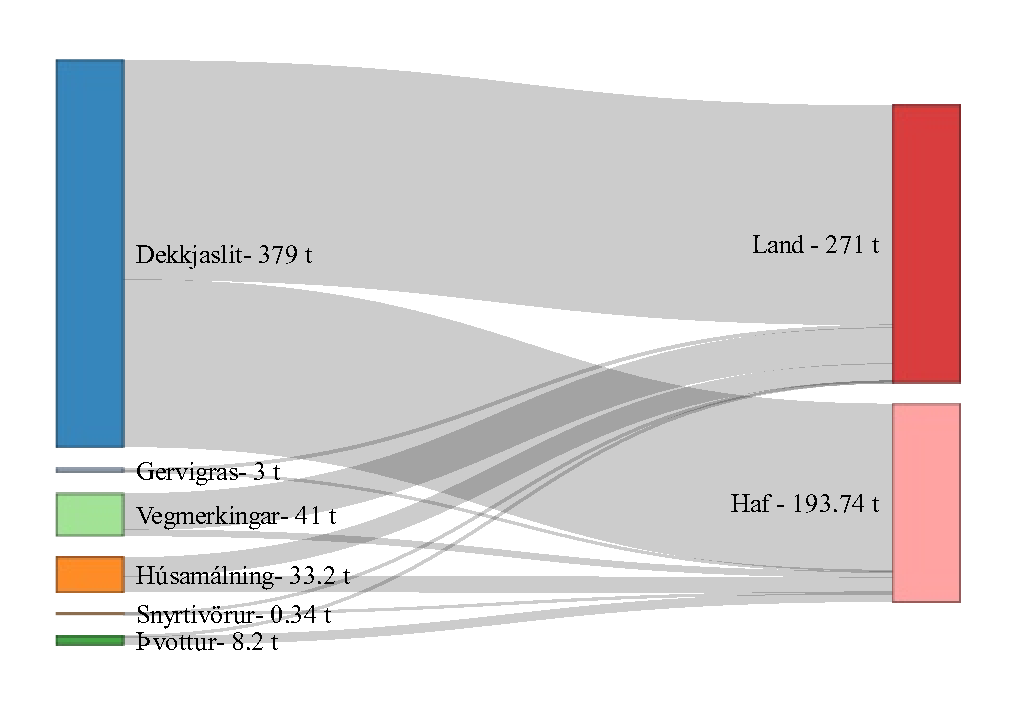
\includegraphics{OrplastHaf_files/figure-latex/unnamed-chunk-2-1} 

}

\caption{Helstu uppsprettur örplasts á Íslandi og skipting þess eftir farleiðum í haf eða í jarðveg. Byggt á lægra mati (sjá meginmál).}\label{fig:unnamed-chunk-2}
\end{figure}

\textbf{Farleiðir örplasts} til hafs eru ólíkar eftir uppsprettum og misflókið er að meta stærð þeirra. Sumar farleiðir fara óhindraðar í hafið líkt og frárennsli úr þvottavélum (í öllum þéttbýlum landsins sem eru við sjó). Affallsvatn frá vegum í þéttbýli á einnig að miklu leyti greiða leið í hafið en vegryk lendir líka að stórum hluta í jarðvegi og ekki er gott að segja til um hvar það endar. Sama á við um málningarflyksur frá háþrýstiþvotti húsa og fleiri uppsprettur í þéttbýli. Það örplast sem lendir í jarðvegi er álitið standa fyrir utan svið þessarar skýrslu þar sem plast er ekki vatnsleysanlegt og situr því að öllum líkindum eftir í jarðveginum og berst ekki í hafið. Helstu farleiðir eru því með rennandi vatni gegnum skólp og ræsi.

\textbf{Í hafinu} brotnar örplast mjög hægt niður þar sem hitastig er lágt í sjónum og útfjólubláir geislar sólar berast aðeins að takmörkuðu leyti í efstu sjávarlögin en ekki á meira dýpi. Það kemur því kannski ekki á óvart að mikil uppsöfnun örplasts er á hafsbotni en einhver mesti þéttleiki örplastagna sem fundist hefur á hafsbotni var við Svalbarða á yfir 2,5 km dýpi sem bendir til þess að örplast berist í miklu magni með sjávarstraumum og jafnvel hafís.

\textbf{Afdrif örplasts} eru að miklu leyti enn ókunn. Það er vel þekkt að það tekur langan tíma fyrir plast að eyðast í umhverfinu og sérstaklega þar sem lítillar birtu gætir og hitastig er lágt. Sundrun plasts (í vatn og koltvísýring) er oftast ekki í það stórum stíl að vert sé á að minnast í skýrslu sem þessari. Sólarljós getur þó valdið talsverðri sundrun á plastefnum í vegmerkingum og utanhússmálningu svo að þær málningarflyksur sem staðið hafa úti í nokkurn tíma innihalda ekki það magn af plasti sem málningin innihélt upphaflega. Það er vandmeðfarið að ætla að skilgreina örplastagnir út frá hlutfallslegu plastinnihaldi þeirra en það er þó ein af fjöldamörgum áskorunum sem rannsóknarfólk stendur frammi fyrir. Í þessari skýrslu er það gert varðandi málningu og vegmerkingar en ekki hjólbarða til dæmis.

Sumar uppsprettur var ekki hægt að leggja mat á vegna skorts á gögnum eða rannsóknum á því hvernig plastrusl í umhverfinu verður að örplasti. Þar ber hæst að nefna losun örplasts úr fjörum en erfitt er að áætla heildarmagn plasts í fjörum og hraða sundrunar þess í örplast. Fjörur geta verið líkt og mulningsvélar fyrir örplast ef stórt plastrusl er ekki fjarlægt úr þeim. Þá ber að nefna að þó svo að almennt sé talin minni hætta fyrir lífverur að innbyrða örplast miðað við stærra plast eru áhrif þess á lífverur og vistkerfi enn óráðin.

\hypertarget{almennt-um-plast}{%
\chapter{Almennt um plast}\label{almennt-um-plast}}

\hypertarget{grunneining-plasts-fjolliur-plastefna}{%
\section*{Grunneining plasts: fjölliður plastefna}\label{grunneining-plasts-fjolliur-plastefna}}
\addcontentsline{toc}{section}{Grunneining plasts: fjölliður plastefna}

Einn stærsti áhrifavaldur 20. aldarinnar á daglegt líf fólks var uppgötvun og hönnun plasts og óhætt er að segja að kaflaskil hafi átt sér stað í framhaldi af því að plastefnið Bakelite var fundið upp árið 1909. Plast leysti af hólmi mörg önnur efni í iðnaði og á heimilum vegna þess, fyrst og fremst, hve ódýrt það er í framleiðslu og hversu slitsterkt það er. Vegna margvíslegra eftirsóttra eiginleika plasts hefur það verið aðlagað að flestum kimum í mannlegu samfélagi. Frá því fjöldaframleiðsla þess hófst er talið að yfir 8 miljarðar tonna hafi verið framleiddir í heiminum og meirihluti þess endað sem úrgangur\textsuperscript{\protect\hyperlink{ref-geyer2017production}{1}}. Plast brotnar ekki auðveldlega niður\footnote{Niðurbrot (e. degradation og fragmentation) er ólíkt sundrun (e. mineralization). Niðurbrot er þegar plast brotnar í minni einingar en niðurbrot er þegar grunneining efnisins breytist.} í náttúrunni og safnast því upp þar með ófyrirséðum afleiðingum.

Það sem við köllum plast í daglegu tali er almennt blanda af fjölliðum plastefna og bætiefnum en hin síðarnefndu gefa plastinu ýmsa eiginleika sem auka notagildi þess. Fjölliður plastefna eru framleiddar úr einliðum sem eru yfirleitt ekki nema nokkur atóm að stærð eins og t.d. etylen sem hefur efnaformúluna \(C~2H~4\). Hver fjölliða getur verið samsett úr þúsundum einliða og er hægt að framleiða fjölmargar ólíkar plastgerðir úr mismunandi samsetningum einliða. Fjölliða etýlens kallast því t.d. pólýetýlen og hefur efnaformúluna \((C~2H~4)~n\).

Til að taka dæmi um fjölbreytta eðliseiginleika mismunandi lengda fjölliða þá er pólýetýlen vaxkennt þegar fjölliðan er samsett úr nokkur hundruð einliðum en þegar þær eru í hundruð þúsunda tali er pólýetýlenið hart plast\textsuperscript{\protect\hyperlink{ref-Andrady2017}{2}}. Annað dæmi er stýren sem er einliða á vökvaformi við stofuhita en þegar margar einliður eru settar saman með efnahvörfum verða til fjölliður efnisins, pólýstýren, sem er betur þekkt á íslensku sem frauðplast \ref{fig:styren}). Sama á við um bútadíen sem er gaskennt efni í einliðuformi en í fjölliðuformi er það byggingareining gervigúmmís. Einnig er hægt að blanda mismunandi plastefnum saman og sem dæmi er hægt að blanda bútadíen og stýren saman til að mynda stýren-bútadíen gúmmí, sem er ein af grunneiningum hjólbarða. Þetta eru einungis örfá dæmi af fjölmörgum um hvernig fjölliður eru samsettar á mismunandi vegu til að framleiða mismunandi plastgerðir\textsuperscript{\protect\hyperlink{ref-Gowariker2005}{3}}.

\begin{figure}

{\centering 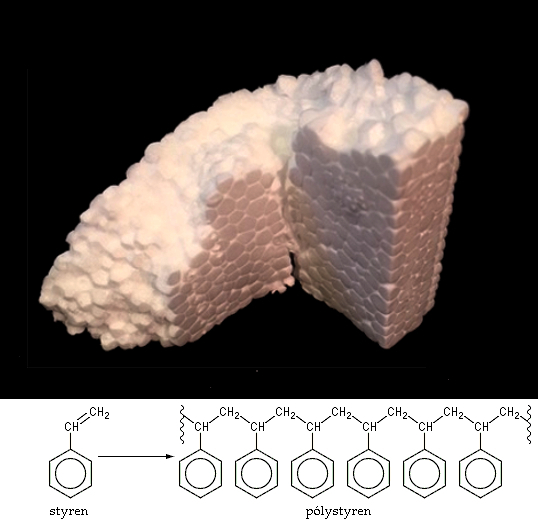
\includegraphics[width=0.7\linewidth]{myndir/polystyrene} 

}

\caption{Einliður stýrens má setja saman með efnahvarfi í langar fjölliður og mynda pólýstýren sem frauðplast er framleitt úr.}\label{fig:styren}
\end{figure}

Mikilvægt er að hafa í huga að hugtakið fjölliða á við um margt fleira en plast og eru t.d. öll prótein fjölliður, auk þess sem viður, ull og silki eru efni sem samanstanda af fjölliðum. Margar náttúrulegar fjölliður, t.d. sellulósi og náttúrulegt gúmmí, eru nýttar á svipaðan máta og plast en teljast ekki til plasts. Mörkin verða þó óljósari t.d. þegar gervigúmmíi er blandað saman við náttúrulegt gúmmí í hjólbörðum. Fjölliður plasts teljast ekki sem náttúrulegar fjölliður en eru engu að síður lífrænar fjölliður þar sem undirstaða byggingar þeirra er úr kolefni\textsuperscript{\protect\hyperlink{ref-Gowariker2005}{3}}. Aðrar ólífrænar fjölliður eru einnig stór hluti af lífi okkar, eins og t.d. gler. Ólíkt plasti er gler efnafræðilega óvirkt efni sem inniheldur ekki óhvarfaðar einliður eða laust bundin niðurbrotsefni og aukaefni sem borist geta út í umhverfið\textsuperscript{\protect\hyperlink{ref-Gudjonsdottir2015}{4}}.

\hypertarget{gerir-plastefna}{%
\section*{Gerðir plastefna}\label{gerir-plastefna}}
\addcontentsline{toc}{section}{Gerðir plastefna}

Plastefni eru af fjöldamörgum gerðum og eru hlutir úr algengustu plastefnunum gjarnan merktir samkvæmt hinu alþjóðlega flokkunarkerfi plastefna (Resin Identification Coding System - RIC) sem hin bandarísku Samtök plastiðnaðarins (Society of the Plastics Industry) komu á fót árið 1988. Sex algengustu plastefnin eru númeruð frá 1-6 en öll önnur plastefni eru sett undir sjöunda flokkinn. Þetta flokkunarkerfi nær því ekki yfir nema takmarkaðan fjölda plastgerða en sé horft til magns af framleiddu plasti ná fyrstu sex flokkanir til um 70\% plastframleiðslu í heiminum\textsuperscript{\protect\hyperlink{ref-geyer2017production}{1}} (sjá töflu \ref{tab:framleidsla}).

\begin{table}[t]

\caption{\label{tab:framleidsla}Alþjóðlegt flokkunarkerfi (RIC) fyrir algengustu plastefnin.}
\centering
\begin{tabular}{ccc}
\toprule
Plastgerð & Skammstöfun (ensk) & Heimsframleiðsla\\
\midrule
Pólýetýlen terefþalat & PET, PETE & 7\%\\
Pólýetýlen - há eðlisþyngd & HD-PE, PE-HD & 15\%\\
Pólývínyl klóríð & PVC & 16\%\\
Pólýetýlen - lág eðlisþyngd & LDPE, PE-LD & 17\%\\
Pólýprópýlen & PP & 23\%\\
\addlinespace
Pólýstýren & PS & 7\%\\
Annað &  & 15\%\\
\bottomrule
\end{tabular}
\end{table}

Plastfjölliður geta verið ýmist hitadeigar (e. thermoplastic) eða hitafastar (e. thermoset) (sjá töflu \ref{tab:plast}). Hitadeigt plast er endurnýtanlegt. Það er hitað upp og mótað undir þrýstingi til að taka á sig þá mynd sem óskað er eftir. Hitafast plast umbreytist með hita og þrýstingi svo samgild tengi myndast sem eru óafturkræf og því er ekki hægt að endurnýta það plast\textsuperscript{\protect\hyperlink{ref-OECD2009}{5}}.

\begin{verbatim}
## NULL
\end{verbatim}

\hypertarget{uppruni-plastefna}{%
\section*{Uppruni plastefna}\label{uppruni-plastefna}}
\addcontentsline{toc}{section}{Uppruni plastefna}

Þrátt fyrir mikinn fjölbreytileika plasts er uppistaðan í meirihluta plastefna framleidd úr einu hráefni, jarðolíu, en það er gert með því að einangra kolefnissambönd jarðolíunnar og vinna úr þeim hinar ýmsu plasteinliður. Að því sögðu er einnig hægt að vinna fjölliður úr plöntuafurðum (e. bioplastics) en umfang þess í dag er lítið og minna en 1\% af heimsframleiðslu plasts. Dæmi um fjölliður úr plöntuafurðum eru sellófan og PLA (polylactic acid), sem er m.a. notað í einnota drykkjarumbúðum, en losun þeirra í umhverfið er engu að síður mengandi þótt þær hafi vissulega ákveðna kosti umfram plast úr jarðolíu\textsuperscript{\protect\hyperlink{ref-karamanlioglu2017abiotic}{6}}. Sem dæmi má nefna að niðurbrot þeirra við umhverfisaðstæður í hafinu gerist hægt og að takmörkuðu leyti\textsuperscript{\protect\hyperlink{ref-tsuji2002environmental-1}{7},\protect\hyperlink{ref-tsuji2002environmental-2}{8}}. Til að setja plastframleiðslu í samhengi við olíuframleiðslu var árið 2009 talið að um 8\% olíu heimsins væri notuð í plast; 4\% sem hráefni og 4\% til að að framleiða orku fyrir framleiðsluferlið\textsuperscript{\protect\hyperlink{ref-hopewell2009plastics}{9}}.

\hypertarget{btiefni-plasts}{%
\section*{Bætiefni plasts}\label{btiefni-plasts}}
\addcontentsline{toc}{section}{Bætiefni plasts}

Plastefni án bætiefna hafa takmarkað notagildi og eru bætiefni nauðsynleg til að ná fram þeim fjölbreytileika plasts sem við þekkjum. Með bætiefnum má ná fram auknum sveigjanleika, vörn gegn útfjólubláum geislum, andoxun, eldvörn og styrk ásamt mörgum fleiri eiginleikum. Áætlað er að bætiefni séu að meðaltali 7\% þyngdar plasthluta en þá eru vefnaðarvörur úr plastefnum ekki meðtaldar\textsuperscript{\protect\hyperlink{ref-geyer2017production}{1}}. Sé notkun bætiefna á heimsvísu skoðuð nánar eru mýkingar-, fylli- og eldvarnarefni um 75\% bætiefna en hver þessara efnaflokka inniheldur mörg mismunandi efni með samskonar tilgang.

\hypertarget{orplast}{%
\chapter{Örplast}\label{orplast}}

Fyrstu staðfestu dæmin um örplast í hafi eru frá því snemma á áttunda áratugnum\textsuperscript{\protect\hyperlink{ref-Waters1972}{10},\protect\hyperlink{ref-Colton1974}{11}} þegar tilkynnt var um litlar pólýstýrenkúlur fljótandi í hafi. Áður hafði fólk gefið því gaum hve plast var slitþolið í sjónum og það fannst æ oftar í maga fugla og annarra dýra. Árið 1991 var bent á að smáar plastagnir úr snyrtivörum bærust út í hafið og olli það áhyggjum fólks\textsuperscript{\protect\hyperlink{ref-zitko1991another}{12}}. Hugtakið míkróplast eða örplast var sett fram 2004\textsuperscript{\protect\hyperlink{ref-Thompson2004lost}{13}} þegar sýni úr sjávarseti voru skoðuð með litrófssjá og um 9 gerðir plasts fundust í þeim. Einnig voru gömul þörungasýni\footnote{þörungasnið eru tekin með háfum með fínum möskva úr efri lögum sjávar úti á opnu hafi sem og nærri ströndum} greind (allt aftur til 1960) og í þeim sást skýrt að eftir því sem framleiðsla á plasti jókst í heiminum fjölgaði plastögnum í hafinu. Birtum vísindagreinum um örplast hefur fjölgað mikið síðustu árin (sjá mynd \ref{fig:pubtrend}) og það hefur fengið mikla athygli yfirvalda og almennings.

\begin{figure}

{\centering 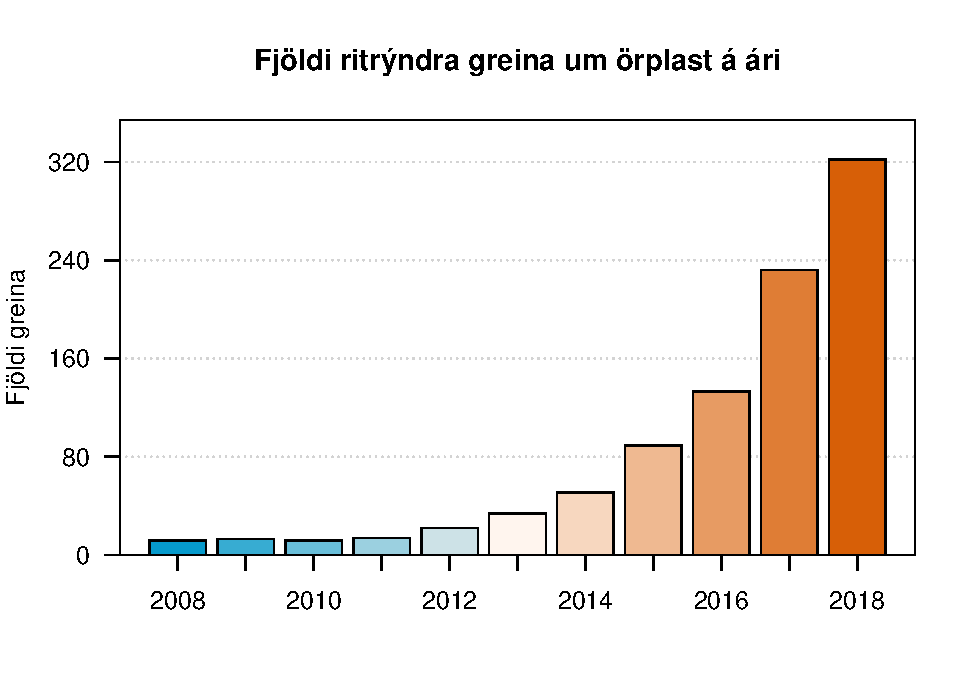
\includegraphics[width=0.8\linewidth]{OrplastHaf_files/figure-latex/pubtrend-1} 

}

\caption{Birtingar alþjóðlegra vísindagreina með örplast sem meginviðfangsefni á árunum 2008 til 2018. Fengið af vef [Web of Knowledge](https://webofknowledge.com).}\label{fig:pubtrend}
\end{figure}

Á landi nær útbreiðsla örplasts til vistkerfa í jarðvegi\textsuperscript{\protect\hyperlink{ref-de2018impacts}{14}} og ferskvatni\textsuperscript{\protect\hyperlink{ref-besseling2017fate}{15}} en losun örplasts á landi er margfalt meiri en til sjávar\textsuperscript{\protect\hyperlink{ref-horton2017microplastics}{16}}. Þrátt fyrir að sýnataka á örplasti í umhverfinu nái yfirleitt einungis til agna stærri en 300 µm og sáralítið sé vitað um útbreiðslu nanóplasts þá hefur örplast engu að síður fundist á yfirborði hafs í öllum heimshlutum\textsuperscript{\protect\hyperlink{ref-eriksen2014plastic}{17},\protect\hyperlink{ref-cozar2014plastic}{18}} og í kjarnasýnum af hafsbotni víða um heim\textsuperscript{\protect\hyperlink{ref-goldberg1997plasticizing}{19}--\protect\hyperlink{ref-woodall2014deep}{21}}. Enn fremur er örplast, líkt og plastrusl almennt, í miklum þéttleika í hringstraumakerfi heimshafanna (e. ocean gyres)\textsuperscript{\protect\hyperlink{ref-law2010plastic}{22}--\protect\hyperlink{ref-lebreton2018evidence}{24}}, ásamt því að safnast fyrir í hafinu á Norðurslóðum\textsuperscript{\protect\hyperlink{ref-cozar2017arctic}{25}} og í hafís\textsuperscript{\protect\hyperlink{ref-obbard2014global}{26}}. Reynt hefur verið að lýsa útbreiðslu örplasts í hafinu og hefur það tekist að einhverju leyti en þörf er á frekari rannsóknum í þeim efnum\textsuperscript{\protect\hyperlink{ref-enders2015abundance}{27}--\protect\hyperlink{ref-auta2017distribution}{29}}. Á heimsvísu hefur verið metið að árlega sé bein losun örplasts í hafið á bilinu 0,8-2,5 milljón tonn\textsuperscript{\protect\hyperlink{ref-boucher2017primary}{30}}.

\hypertarget{skilgreining-orplasts}{%
\section*{Skilgreining örplasts}\label{skilgreining-orplasts}}
\addcontentsline{toc}{section}{Skilgreining örplasts}

Örplast er almennt skilgreint mjög vítt en undir það hugtak ná allar litlar plastagnir minni en 5 mm (í öllum víddum; lengd, hæð eða breidd) svo það á við um kúlulaga agnir, þunnar flyksur og þræði. Örplastagnir eru ýmist framleiddar sem örplast eða verða að örplasti við slit og sundrun stærra plasts í umhverfinu. Ekki er samhljómur um hvort taka eigi undir þetta hugtak vatnsleysanlegar fjölliður eða „hydrogel``\textsuperscript{\protect\hyperlink{ref-Bergmann2015}{31}} en slíkt er notað við gerð á seyru úr skólpi.

\hypertarget{frummynda-og-simynda-orplast}{%
\subsection*{Frummyndað og síðmyndað örplast}\label{frummynda-og-simynda-orplast}}
\addcontentsline{toc}{subsection}{Frummyndað og síðmyndað örplast}

Örplast er gjarnan flokkað í frummyndaðar eða síðmyndaðar agnir eftir því hvernig það berst í umhverfið\textsuperscript{\protect\hyperlink{ref-boucher2017primary}{30},\protect\hyperlink{ref-sundt2014sources}{32}}.

\begin{itemize}
\item
  Síðmyndaðar örplastagnir eru þær sem verða til við sundrun plasts í náttúrunni.
\item
  Frummyndaðar örplastagnir er plast sem berst út í umhverfið sem örplast.
\end{itemize}

Þessi flokkun er óháð hlutverki plastsins og notkun á líftíma þess sem neysluvöru en byggir á sjónarhorni viðtakans sem er umhverfið. Til dæmis þá getur örplast út frá hjólbörðum bæði verið frummyndaðar og síðmyndaðar agnir eftir því hvort um er að ræða veðrun hjólbarða á bryggju (síðmyndað) eða dekkjaagnir sem berast með affallsvatni frá vegum (frummyndað). Sama á við um þræði úr syntetískum fatnaði sem berast til sjávar sem örplast eftir þvott í gegnum skólpkerfi og flokkast þá sem frummyndað örplast rétt eins og annað örplast sem berst með skólpi í hafið t.a.m. örplast úr snyrtivörum.

Frummynduðu örplasti má skipta í tvo flokka eftir því hvort það myndast vegna slits eða notkunar á stærra plasti eða hvort það er framleitt sem örplast. Vísvitandi framleitt örplast er ekki stór hluti örplastmengunar. Það finnst í mörgum neysluvörum og er einnig notað víða við sandblástur en skýrsluhöfundar vita ekki af dæmi þess hérlendis. Örplast sem myndast vegna slits á stærra plasti er langstærsti hlutinn af frummynduðu örplasti. Síðmyndað örplast á við um plast sem er þegar komið út í umhverfið þegar það molnar eða slitnar og verður að örplasti. Það á líka við um örplast sem lekur úr landfyllingum eða jafnvel tilfærslu á örplasti t.d. við upprót á örplasti úr sjávarseti\textsuperscript{\protect\hyperlink{ref-sundt2014sources}{32}}.

\hypertarget{str-orplastagna-i-umhverfinu}{%
\section*{Stærð örplastagna í umhverfinu}\label{str-orplastagna-i-umhverfinu}}
\addcontentsline{toc}{section}{Stærð örplastagna í umhverfinu}

Mikilvægt er að gera greinarmun á mismunandi stærðum örplasts í ljósi mismunandi áhrifa á lífríki eftir stærð\textsuperscript{\protect\hyperlink{ref-velzeboer2014strong}{33}} og erfitt hefur reynst að lýsa nákvæmlega hvernig ólíkir stærðarflokkar örplasts hegða sér í sjónum eða flytjast milli hafsvæða\textsuperscript{\protect\hyperlink{ref-thompson2015microplastics}{34}}. Sem dæmi má nefna að örplastagnir geta komist inn í blóðrásarkerfi skeldýra séu þær nógu litlar\textsuperscript{\protect\hyperlink{ref-browne2008ingested}{35}} og eftir því sem örplastagnir eru minni getur hlutfallslega meira magn eiturefna loðað við þær vegna hærra hlutfalls yfirborðsflatar\textsuperscript{\protect\hyperlink{ref-velzeboer2014strong}{33}}.
Umhverfismælingar ná sjaldnast til minnstu agnanna\textsuperscript{\protect\hyperlink{ref-loder2015methodology}{36}} en lagt hefur verið til að skipta örplasti niður í þrjá flokka á þeim forsendum að viðbúið er að hver stærðarflokkur hegði sér á mismunandi hátt í umhverfinu\textsuperscript{\protect\hyperlink{ref-andrady2011microplastics}{37}}:

\begin{itemize}
\tightlist
\item
  agnir \textless{}50 µm (nanóplast)
\item
  agnir frá 50-500 µm (míkróplast) og
\item
  agnir frá 500 µm-5000 µm (5 mm) (mesóplast)
\end{itemize}

\hypertarget{afdrif-og-rek-orplasts-i-hafinu}{%
\section*{Afdrif og rek örplasts í hafinu}\label{afdrif-og-rek-orplasts-i-hafinu}}
\addcontentsline{toc}{section}{Afdrif og rek örplasts í hafinu}

Mestur þéttleiki örplasts í yfirborðslögum sjávar er nærri uppsprettum þess á landi við þéttbýli og árósa og um 80\% þess er af gerðinni pólýetýlen og pólýprópýlen\textsuperscript{\protect\hyperlink{ref-isobe2014selective}{38},\protect\hyperlink{ref-Gewert2017}{39}} sem falla undir resín-kóða eitt, tvö, fjögur og fimm og eru yfir 60\% af framleiddu plasti í heiminum (líkt og sést í töflu \ref{tab:framleidsla}). Ólíkar gerðir plastefna hafa mismunandi eðlisþyngd og aðeins um helmingur af framleiddu plasti hefur hærri eðlisþyngd en sjór\textsuperscript{\protect\hyperlink{ref-sherrington2016study}{40}} en það hefur áhrif á útbreiðslu þeirra í hafinu\textsuperscript{\protect\hyperlink{ref-andrady2011microplastics}{37}}.

\begin{figure}

{\centering 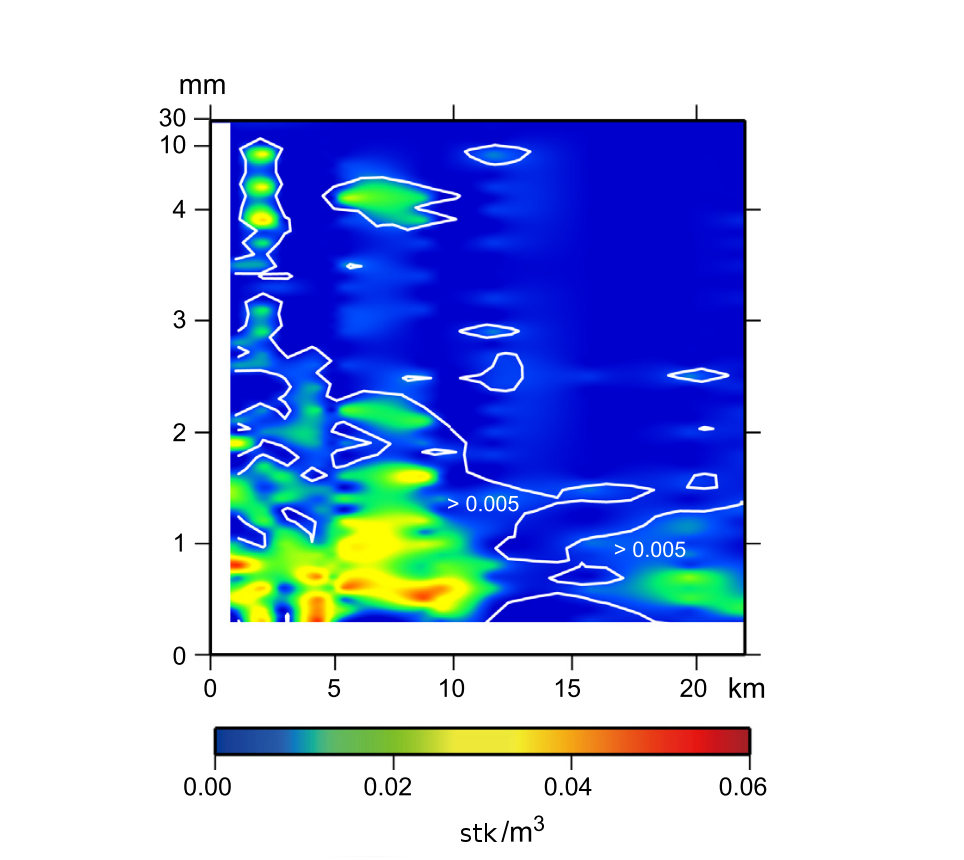
\includegraphics[width=0.8\linewidth]{myndir/DriftDensity_isobe2014} 

}

\caption{Þéttleiki smárra plastagna á reki í hafinu. Lárétti ásinn stendur fyrir fjarlægð frá landi og lóðrétti ásinn stærð plastagnanna sem fengust í háf við yfirborðið. Litaskalinn táknar þéttleika agnanna. Þéttleiki yfir 0,005 stk/m~3~ er innan línanna á myndinni [@isobe2014selective].}\label{fig:DriftDensity}
\end{figure}

Í hafinu, líkt og í vatni almennt, verka ólíkir kraftar á mjög smáar agnir miðað við stærri hluti. Stærri hlutir eru háðir tregðukröftum en smærri hlutir verða aðallega fyrir áhrifum seigjukrafta. Það má útskýra með svokallaðri Reynoldstölu (\emph{Re})\textsuperscript{\protect\hyperlink{ref-levinton1995marine}{41}} en stórir hlutir á mikilli ferð hafa hátt \emph{Re} og þurfa mikla tregðu til að stoppa á meðan smáir hlutir á lítilli ferð hafa lágt \emph{Re}\textsuperscript{\protect\hyperlink{ref-levinton1995marine}{41}} og geta því svifið í vatni líkt og í þyngdarleysi. Þar sem núningskraftar sjávar verka með hverfandi hætti á örplast flýtur það ekki upp á yfirborðið hafi það borist í dýpri lög sjávar ólíkt stærra plasti jafnvel þótt það hafi lægri eðlisþyngd en sjórinn\textsuperscript{\protect\hyperlink{ref-isobe2014selective}{38}}. Örplast getur því sokkið burt séð frá eðlisþyngd þess, það berst bara með hreyfingum sjáva og sjávarstraumum. Það gæti verið ein af ástæðum þess að örplast rekur síður á land en stórt plast og finnst í hærra hlutfalli gagnvart stærra plasti úti á rúmsjó\textsuperscript{\protect\hyperlink{ref-isobe2014selective}{38}} (sjá mynd \ref{fig:DriftDensity}) en rek af hafi á fjörur vegna ölduhreyfinga er hraðara eftir yfirborði sjávar og minnkar með auknu dýpi, skv. lögmáli Stokes\textsuperscript{\protect\hyperlink{ref-stokes1851effect}{42}}.

Örplast er ólíkt flestum öðrum ögnum sem svífa um í sjónum vegna þess hve lengi það endist. Vatnsfælið yfirborð örplasts nýtist sem búsvæði fyrir örverur af ýmsum toga og hefur verið kallað á ensku „plastisphere``\textsuperscript{\protect\hyperlink{ref-Zettler2013}{43}}. Með örplasti hefur því orðið til ný leið fyrir útbreiðslu tegunda á milli hafsvæða.

\hypertarget{niurbrot-orplasts-i-hafinu-og-upptaka-i-fukejur}{%
\section*{Niðurbrot örplasts í hafinu og upptaka í fæðukeðjur}\label{niurbrot-orplasts-i-hafinu-og-upptaka-i-fukejur}}
\addcontentsline{toc}{section}{Niðurbrot örplasts í hafinu og upptaka í fæðukeðjur}

Rannsóknir á niðurbroti plasts í umhverfinu voru lítið stundaðar þar til um aldamótin síðustu. Mestar upplýsingar um hrörnun plasts koma frá sjónarhóli iðnaðarins um endingu og slit á ýmsum gerðum af plasti.
Orðið niðurbrot á við um á eðlis- eða efnafræðilegar breytingar á efni og er óafturkræft ferli. Niðurbrot leiðir til verulegra breytinga á byggingu plastsins sem kemur fram í breyttum eiginleikum þess (t.d. það verður stökkt eða laust í sér, mólmassi lækkar) eða sundrun\textsuperscript{\protect\hyperlink{ref-ISO472}{44}}. Sundrun (e. mineralization) er algjört niðurbrot lífrænna efnasambanda yfir í vatn og koltvísýring (og metan við loftóháð skilyrði)\textsuperscript{\protect\hyperlink{ref-SameiginlegaEes-nefndin2007}{45}} og er lokaskref niðurbrotsferilsins.

Niðurbrotsferli plasts, þ.m.t. örplasts, er breytilegt eftir efnabyggingu þess og verulega háð umhverfisaðstæðum\textsuperscript{\protect\hyperlink{ref-gewert2015pathways}{46}} en það gerist mjög hægt í umhverfinu og oft að takmörkuðu leiti\textsuperscript{\protect\hyperlink{ref-barnes2009accumulation}{47}}. Stærsti áhrifaþátturinn á niðurbrot plasts í hafi er sólarljós í samspili við súrefni (e. photo oxidative degradation), vatnsrof og lífrænt niðurbrot fylgja þar á eftir\textsuperscript{\protect\hyperlink{ref-gewert2015pathways}{46}} og hærra hitastig hraðar ferlinu (sjá mynd \ref{fig:flowchart}).

Fjölmargir þættir hafa áhrif á eðli niðurbrotsins en sem dæmi hefur gerð grunneiningar fjölliðukeðjunnar plastsins mikil áhrif, þ.e. eftir því hvort grunnkeðjan er eingöngu kolefniskeðja eða með heterófrumeind (t.d. pólýetýlen terefþalat og pólýúretön) sem gerir fjölliðurnar mis-berskjaldaðar fyrir niðurbroti\textsuperscript{\protect\hyperlink{ref-Singh2008}{48}}.

\begin{figure}

{\centering 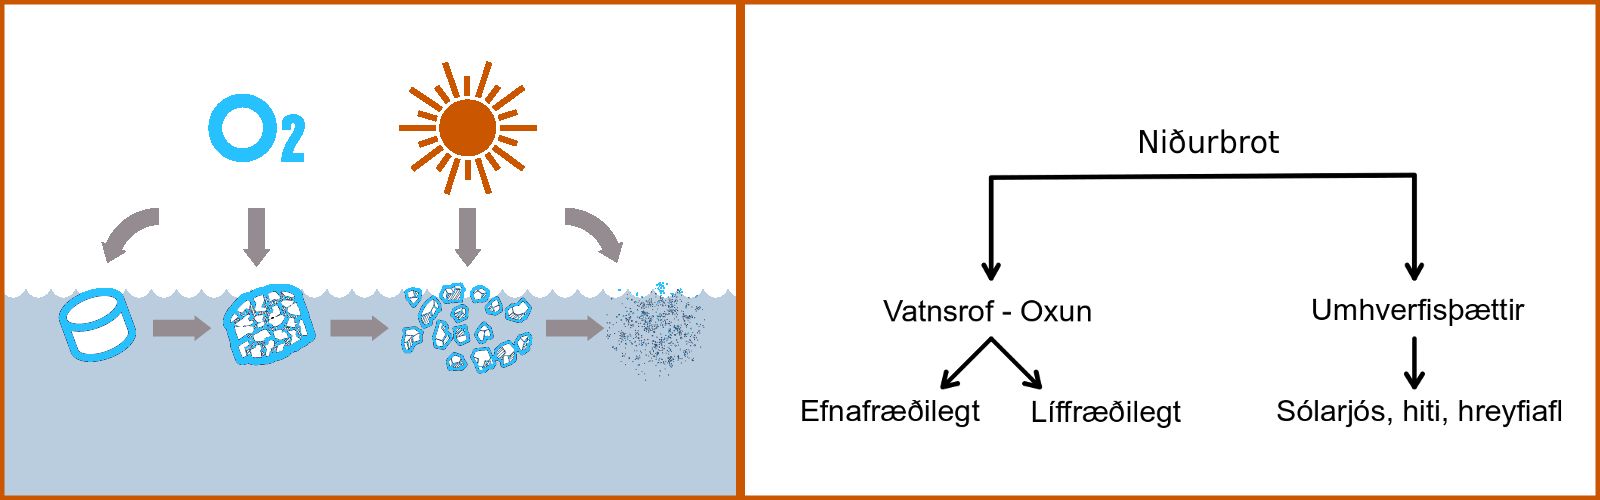
\includegraphics[width=1\linewidth]{myndir/small-plastics_FLAEDIRIT} 

}

\caption{Niðurbrot plasts í hafinu, helstu leiðir. Mynd unnin eftir (Fotopoulou 2017 og af [vefnum](https://www.nurdlehunt.org.uk/)) [@Fotopoulou2017; @nurdle].}\label{fig:flowchart}
\end{figure}

Í sinni einföldustu mynd eru fjölliður plastefna formlausar (e. amorphous) og plastið því mjúkt en eftir því sem fjölliðurnar eru lengri þá verður plastið stífara. Í sinni formlausu mynd geta fjölliður engu að síður verið ýmist einfaldar keðjur (e. linear polymer), greinóttar (e. branched polymer) eða samtengdar með samgildum tengjum (e. cross-linked polymer) og hefur það áhrif á stífleika plastsins. Kristaleiningar fjölliða eru þolnari gagnvart niðurbroti en formlaus hluti þeirra, sem veldur því að niðurbrot er ójafnt milli einstakra hluta plastfjölliðanna\textsuperscript{\protect\hyperlink{ref-andrady2017plastic}{49}}. Almennt brotnar plast fyrr niður í kringum þessi formlausu svæði bæði vegna lífrænna og ólífrænna þátta en formlausir hlutar fjölliða eru t.d. viðkvæmari gagnvart sólarljósi en þeir sem eru í kristalformi. Þetta leiðir af sér að niðurbrot plasts með hátt kristalhlutfall gerist á öðruvísi máta en hjá plasti með lágt kristalhlutfall\textsuperscript{\protect\hyperlink{ref-andrady2017plastic}{49}} og sífellt smærri agnir örplasts myndast við niðurbrot.

Örverur geta einnig átt þátt í niðurbroti örplasts með meltingarensímum\textsuperscript{\protect\hyperlink{ref-shah2008biological}{50}} (sjá mynd \ref{fig:Plastpit}), einkum við hagstæðar aðstæður á rannsóknarstofu\textsuperscript{\protect\hyperlink{ref-pacco2017biodegradation}{51}}. Vöxtur þeirra er þó minni við umhverfisaðstæður, t.d. í sjó þar sem lágt hitastig takmarkar eða hægir á niðurbroti af þeirra völdum\textsuperscript{\protect\hyperlink{ref-andrady2011microplastics}{37},\protect\hyperlink{ref-barnes2009accumulation}{47}}.

\begin{figure}

{\centering 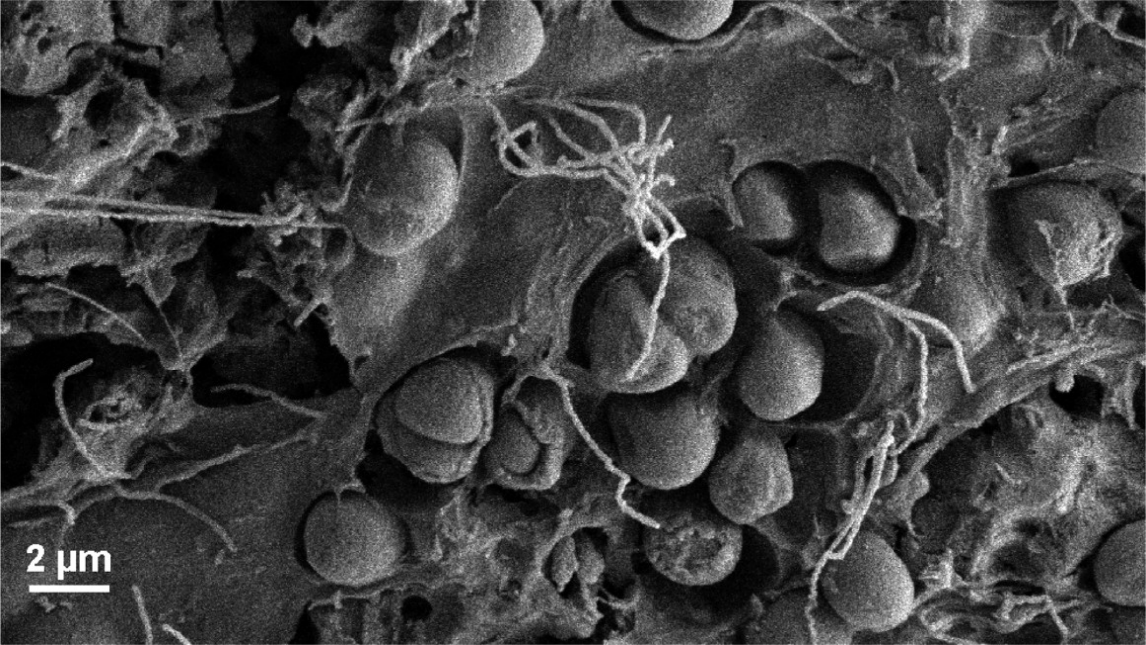
\includegraphics[width=0.8\linewidth]{myndir/Plast_pit} 

}

\caption{Ógreindar bakteríur grafnar inn í yfirborð plastagna sem fundust í sýnum úr hafi [@Zettler2013].}\label{fig:Plastpit}
\end{figure}

Við niðurbrot plastefna losna ýmis afleiðuefni, t.d. karboxílsýrur, aldehýð, ketónar, fenól og bensen\textsuperscript{\protect\hyperlink{ref-gewert2015pathways}{46}} og er það því viðbót við mengandi áhrif bætiefna og efna sem loða við plastið í umhverfinu.
Nær allar gerðir plasts eru framleiddar með mismunandi íblöndunarefnum sem hafa áhrif á það hversu vel plastið brotnar niður og sundrast í umhverfinu\textsuperscript{\protect\hyperlink{ref-gewert2015pathways}{46}} þar sem meginþorri þeirra er gerður til þess að varna hrörnun plastsins.

Erfitt er að segja til um líftíma örplasts í umhverfinu en þó hefur verið sýnt fram á að örplast á yfirborði sjávar getur verið þar í langan tíma án þess að brotna fyllilega niður\textsuperscript{\protect\hyperlink{ref-brandon2016long}{52}}. Enn síður brotnar það niður í sjávarseti en sjávarbotn í djúphöfunum gæti verið stærsti viðtaki örplasts á jörðinni\textsuperscript{\protect\hyperlink{ref-woodall2014deep}{21}}. Á sjávarbotni á grunnsævi eru næringarefni og lífvirk efni í meira mæli en í djúpsjávarseti úti á rúmsjó. Þar er upprót á botnseti líka meira og má því leiða líkur að því að möguleikar á niðurbroti örplasts séu meiri á grunnsævi en í orkulægri vistkerfum á djúpsjávarbotni\textsuperscript{\protect\hyperlink{ref-Nozari2016}{53}}.

Niðurbrot plasts er langtum hraðara í fjörum heldur en í sjó en sjórinn veitir skjól gagnvart veðrun og hefur minna súrefnisinnihald en andrúmsloftið\textsuperscript{\protect\hyperlink{ref-andrady2011microplastics}{37}}. Þar að auki geta ásætur, sem hafa betri vaxtarskilyrði í hafinu en í fjöru, hægt á niðurbrotsferlinu með því að hindra aðkomu sólarljóssins að plastinu\textsuperscript{\protect\hyperlink{ref-o2010degradation}{54},\protect\hyperlink{ref-muthukumar2011fouling}{55}}. Strandhreinsanir eru því mikilvægur þáttur í því að koma í veg fyrir myndun örplasts og losun bæti- og afleiðuefna í umhverfið.

Ósamræmi er á milli þess hve mikið magn af plasti er framleitt og berst í hafið og þess sem mælist sem örplast\textsuperscript{\protect\hyperlink{ref-cozar2014plastic}{18}}. Þetta á sérstaklega við um smærri örplastagnir (sjá mynd \ref{fig:cozer}). Eftir því sem örplastagnir brotna í minni einingar verða þær mögulega innbyrtar af æ fleiri hópum lífvera\textsuperscript{\protect\hyperlink{ref-cozar2014plastic}{18}}. Það er því alls ekki ljóst hve stór hluti örplastagna er tekinn upp í fæðukeðjur í hafinu, hve stór hluti þeirra sundrast eða hve stór hluti þeirra sekkur til botns. Afdrif örplasts minni en 20 µm eru ókunn vegna þess að sýnatökuaðferðir hafa enn ekki verið þróaðar með fullnægjandi hætti\textsuperscript{\protect\hyperlink{ref-RENNER201855}{56}}. Ekki er mikið vitað um niðurbrot örplasts í nanóplast, einkum þar sem sýnataka er takmörkunum háð, en þar sem nanóplast getur myndast við slit plasts á rannsóknarstofu má gera ráð fyrir að það geti myndast og verið til staðar í umhverfinu\textsuperscript{\protect\hyperlink{ref-lambert2016formation}{57}}.

\begin{figure}

{\centering 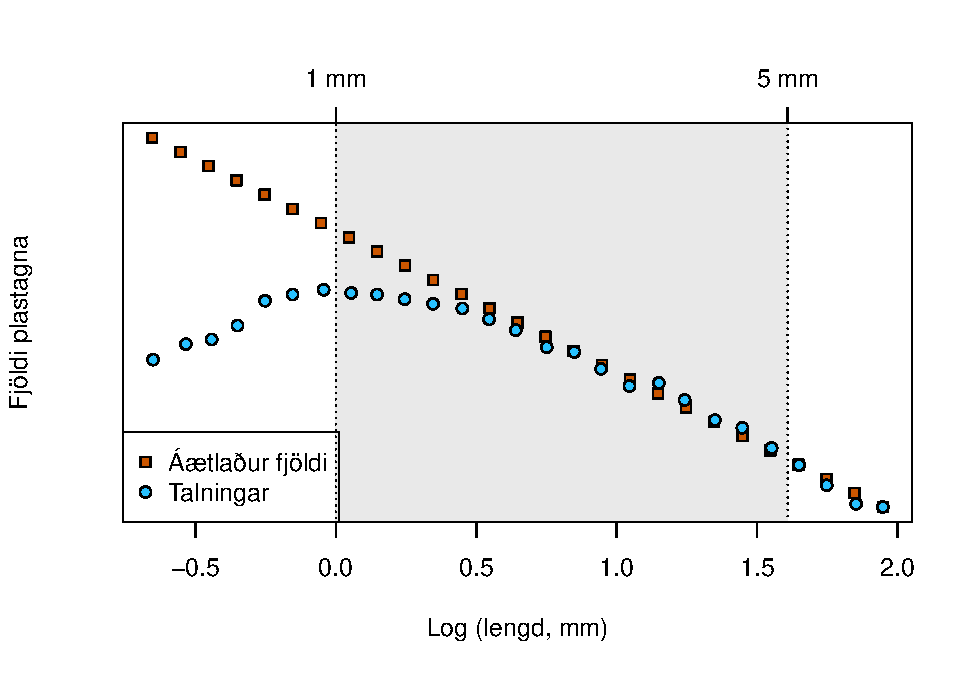
\includegraphics[width=0.8\linewidth]{OrplastHaf_files/figure-latex/cozer-1} 

}

\caption{Mæld og áætluð stærðardreifing (lograskali) örplastagna í yfirborðslögum sjávar í svokölluðum plastflákum. Áætluð gildi voru einungis metin út frá niðurbroti stærra plasts. Skyggða svæðið sýnir stærðarmörkin frá 1 mm til 5 mm. (Mynd unnin eftir Cozar 2014 [@cozar2014plastic])}\label{fig:cozer}
\end{figure}

\hypertarget{tknileg-umra-um-synatokur}{%
\subsection*{Tæknileg umræða um sýnatökur}\label{tknileg-umra-um-synatokur}}
\addcontentsline{toc}{subsection}{Tæknileg umræða um sýnatökur}

Örplast í umhverfinu er misjafnt að lögun, stærð og lit og hefur ólíka efnasamsetningu\textsuperscript{\protect\hyperlink{ref-phuong2016there}{58}} sem meðal annars gerir það erfitt að samræma staðlaðar aðferðir við söfnun og greiningu þess.
Margar ólíkar greiningaraðferðir eru mögulegar en henta misvel eftir stærð agnanna og eðlisþyngd\textsuperscript{\protect\hyperlink{ref-hepso2018experimental}{59}}. Einföld athugun með víðsjá og smásjá er enn mjög gagnleg aðferð\textsuperscript{\protect\hyperlink{ref-hepso2018experimental}{59},\protect\hyperlink{ref-SONG2015202}{60}} en agnir sem líta út eins og flyksur eru þá frekar vantaldar og þráðlaga örplast oftalið\textsuperscript{\protect\hyperlink{ref-SONG2015202}{60}}. Hins vegar eru gegnsæjar eða hvítar agnir oft taldar sem syntetískar fjölliður, líkt og pólýetýlen og pólýprópýlen, í litrófssjá (Fourier Transformed- Infra Red, eða Raman)\textsuperscript{\protect\hyperlink{ref-SONG2015202}{60}}. Litun sýnanna með Nílar rauðum lit ásamt skoðun flúrljómandi sýna í smásjá hefur gefið góða raun við að greina örplastagnir af ólíkri lögun og bæði á míkró- og nanóskala en þó eru vandamál tengd myndgreiningu og menguðum sýnum\textsuperscript{\protect\hyperlink{ref-SHIM2016469}{61}}. Rafeindasmásjár gefa upplýsingar um stærð og lögun örplasts og jafnvel efnasamsetningu sé röntgengeisla-ljómun notuð samhliða (Energy X-ray dispersion spectroscopy)\textsuperscript{\protect\hyperlink{ref-bitam2014bio2}{62}}.

\begin{figure}

{\centering 
\includegraphics[width=1\linewidth]{myndir/synataka} 

}

\caption{Yfirlit yfir aðferðir við sýnatökur á plasti frá nanóplasti og upp úr. FTIR stendur fyrir "Fourier Transformed- Infra Red" og FFF fyrir "Field Flow Fractionation" (sjá Mintenig 2016 [@Mintenig2016]).}\label{fig:FTIR}
\end{figure}

Niðurstöður litrófsgreininga á örplasti passa stundum ekki við þekkt sýni þar sem veðrun á yfirborði agnanna úr umhverfinu gefur ólíkar niðurstöður.
Hitasundrun með gasgreini tengdum massagreini (pyrolysis gas chromatography -- mass spectrometry (Pyr-GC/MS)) þar sem sýnin eru hituð þannig að efnasambönd brotna niður við súrefnisfirrtar aðstæður þau aðgreind í gasgreini og greind í massagreini\textsuperscript{\protect\hyperlink{ref-k22014bio2}{63}}. Helstu kostir við þessa aðferð (Pyr-GC/MS) eru að ekki þarf að einangra sýnin, syntetísku fjölliðurnar og residual matrix geta farið saman í hitasundrun og gefið eigindlegar og nokkuð magnbundnar niðurstöður\textsuperscript{\protect\hyperlink{ref-Fischer2017}{64}}.

\hypertarget{farvegir-orplasts}{%
\chapter{Farvegir örplasts}\label{farvegir-orplasts}}

Rennandi vatn er helsti farvegur örplasts á landi til sjávar\textsuperscript{\protect\hyperlink{ref-unice2019characterizing1}{65}} hvort sem það rennur eftir ám og lækjum eða niður ræsi og með skólpi. Aðrar farleiðir örplasts eru taldar upp í töflu \ref{tab:fartafla}. Margar gerðir örplasts flytjast að einhverju leyti með fleiri farvegum en einum en þrátt fyrir það eru ákveðnar uppsprettur örplasts einkennandi fyrir hvern farveg. Hér er því sett fram samantekt á því hvaða uppsprettur örplasts eru einkennandi fyrir hvern farveg, einkum þegar litið er til hlutfalls af heildarlosun hverrar uppsprettu. Þetta er því ekki tæmandi listi en er engu að síður hagnýt samantekt fyrir kortlagningu örplastmengunar innan einstakra vatnasvæða á Íslandi.

Mesta magn örplasts sem fundist hefur hingað til í sjávarbotnsseti var rétt vestur af Svalbarða á 2,5 til 5,5 km dýpi\textsuperscript{\protect\hyperlink{ref-Bergmann2017}{66}}. Útilokað er að sú mengun sé staðbundin og sýnir fram á að örplast berst með hafstraumum á fjarlæg hafsvæði. Örplast getur því einnig borist inn á íslenskt hafsvæði með hafstraumum. Til dæmis með flæði Atlantshafssjávar úr suðri en það flæði er árstíðabundið og mismikið milli ára\textsuperscript{\protect\hyperlink{ref-Strait2005a}{67}} líkt og á við um hafstrauma sem fara í kringum Ísland og geta borið örplast frá helstu uppsprettum á suð- vesturhorni landsins, réttsælis með landinu norður fyrir Vestfirði\textsuperscript{\protect\hyperlink{ref-Astthorsson1994}{68}} á svæði þar sem mengun er ekki eins mikil frá landi vegna fámennari byggða.

\begin{tabular}{ccc}
\toprule
Gerð farvegs & Farvegur & Uppsprettur í farvegi\\
\midrule
Rennandi vatn & Fráveita: skólp og ofanvatn & Fatnaður\\
Rennandi vatn & Fráveita: skólp og ofanvatn & Snyrtivörur\\
Rennandi vatn & Fráveita: skólp og ofanvatn & Plastframleiðsla\\
Rennandi vatn & Fráveita: skólp og ofanvatn & Gervigrasvellir\\
Rennandi vatn & Fráveita: skólp og ofanvatn & Leiksvæði\\
\addlinespace
Rennandi vatn & Fráveita: skólp og ofanvatn & Skósólar\\
Rennandi vatn & Fráveita: skólp og ofanvatn & Vegryk*\\
Rennandi vatn & Fráveita: skólp og ofanvatn & Málning\\
Rennandi vatn & Ár, lækir og skurðir & Heyrúlluplast\\
Rennandi vatn & Ár, lækir og skurðir & Haglaskot\\
\addlinespace
Rennandi vatn & Ár, lækir og skurðir & Plastrusl\\
Andrúmsloft & Vindur & Vegryk*\\
Hafið & Hafstraumar/sjávarföll & Veiðarfæri\\
Hafið & Hafstraumar/sjávarföll & Búnaður í sjókvíaeldi\\
Hafið & Hafstraumar/sjávarföll & Plastrusl í hafinu\\
\addlinespace
Annað & Sigvatn & Örplast frá urðunarstöðum\\
Annað & Landgræðsla & Áburður úr seyru\\
Annað & Snjómokstur & Vegryk*\\
\bottomrule
\end{tabular}

Á landi berst örplast með vatni, vindi og með athöfnum manna. Helsta uppspretta örplasts sem dreifist með vindi er slit hjólbarða bifreiða sem sest við vegi\textsuperscript{\protect\hyperlink{ref-Cadle1978}{69}}. Dreifing örplasts getur einnig gerst með notkun seyru til landgræðslu en algengt er að hún innihaldi örplast úr snyrtivörum\textsuperscript{\protect\hyperlink{ref-zitko1991another}{12}} og plastúrgangi sem berst í skólphreinsistöðvar og rotþrær. Það sama getur gilt um jarðbæti unninn úr úrgangi sem inniheldur plast, einkum ef ekki er gert ráð fyrir hreinsun örplasts í míkró- og nanóstærð.

\begin{figure}

{\centering 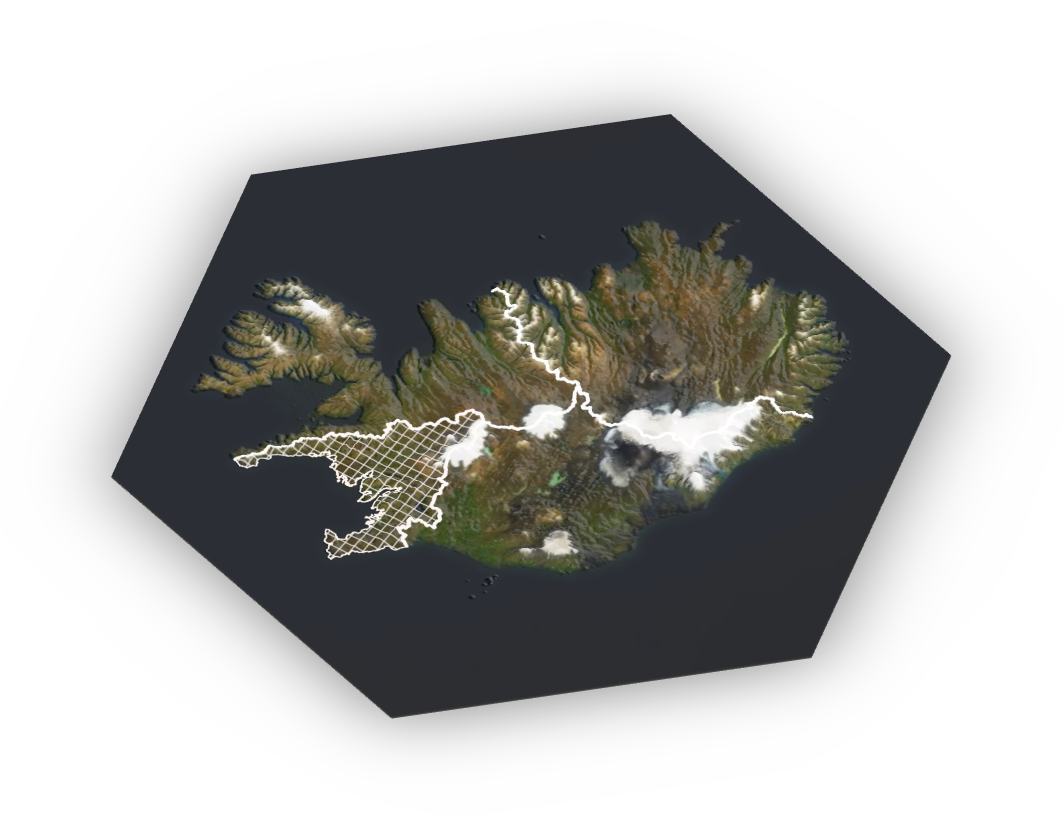
\includegraphics[width=1\linewidth]{myndir/map} 

}

\caption{Fjögur megin vatnasvæði Íslands. Skálínurnar liggja yfir vatnasvæði nr. 104 á suðvesturhorni landsins}\label{fig:vatnasvidsv}
\end{figure}

Þegar losun örplasts á Íslandi er skoðuð er rétt að taka suðvestur horn landsins út fyrir sviga. Þar sem helsta farleið örplasts er með rennandi vatni er hér notast við skiptingu íslenska vatnaumdæmisins í fjögur meginvatnasvæði\textsuperscript{\protect\hyperlink{ref-Bj2012}{70}}. Á suðvesturhorni landsins er vatnasvæði sem rennur í Faxaflóa (sjá mynd \ref{fig:vatnasvidsv}). Á því svæði býr um 3/4 landsmanna\footnote{\url{http://px.hagstofa.is/pxis/pxweb/is/Ibuar/Ibuar__mannfjoldi__2_byggdir__Byggdakjarnar/MAN03106.px/table/tableViewLayout1/?rxid=830c3a84-47bf-4090-8227-4c683a2f2770}} og þar er summa \href{http://www.vegagerdin.is/upplysingar-og-utgafa/umferdin/adferdarfraedi-talninga/}{árdagsumferðar} rúmir 3/4 hlutar á landsvísu. Flatarmál bygginga þar er yfir 50\% flatarmáls allra bygginga á landsvísu\textsuperscript{\protect\hyperlink{ref-OpenStreetMap}{71}} en flatarmál málaðra flata eflaust enn meiri vegna byggingarhæðar. Flestir landsmenn fara til Reykjavíkur reglulega til að sækja þjónustu sem þar er í boði, nær allar vöruflutningar eru um svæðið og nærri allt millilandaflug. Þrír stórir slippir af fjórum eru á Höfuðborgarsvæðinu og í Grindavík. Það er því rík ástæða til að skoða þetta svæði betur.

\hypertarget{skolp-og-rsi}{%
\subsection*{Skólp og ræsi}\label{skolp-og-rsi}}
\addcontentsline{toc}{subsection}{Skólp og ræsi}

Fæst bæjarfélög á Íslandi hreinsa skólp að nokkru leyti \ref{fig:skolp} en þar sem skólphreinsistöðvar eru á höfuðborgarsvæðinu fer skólp frá flestum landsmönnum í gegnum hreinsun og hefur því hlutfall þeirra sem búa á svæðum þar sem skólp er hreinsað margfaldast á síðustu áratugum\textsuperscript{\protect\hyperlink{ref-uxdeoruxf0arson2012}{72}}.

\begin{figure}

{\centering 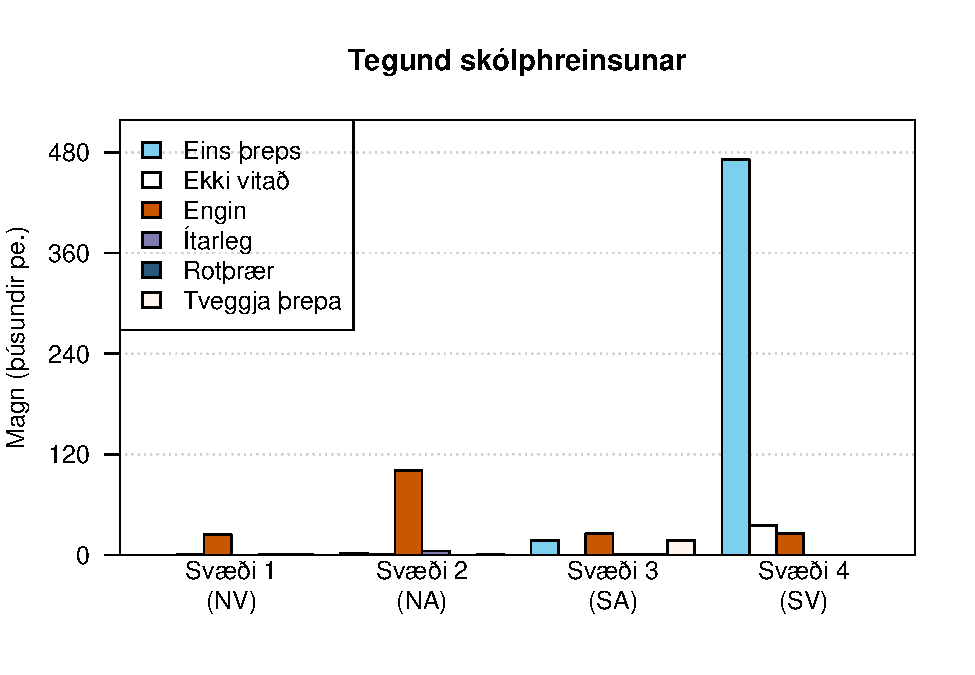
\includegraphics[width=1\linewidth]{OrplastHaf_files/figure-latex/skolp-1} 

}

\caption{Tegund skólphreinsunar skipt eftir fjórum flokkum náttúrulegra yfirborðsvatnshlota. Unnið upp úr samantekt á stöðu skólpmála á Íslandi árið 2014 [@Umhverfisstofnun2017].}\label{fig:skolp}
\end{figure}

Skólphreinsun í Reykjavík er svokölluð fyrsta stigs hreinsun,\footnote{„Hreinsunin uppfyllir að öllum líkindum ekki þær kröfur sem gerðar eru til eins þreps hreinsunar í reglugerð um fráveitur og skólp``\textsuperscript{\protect\hyperlink{ref-Umhverfisstofnun2017}{73}}} þar sem efni á föstu formi eru aðskilin vatni með botnfellingu, fleytingu eða notkun rista. Þær eru í blönduðu kerfi sem tekur á móti skólpi ásamt ofanvatni og með yfirfalli þegar álag er mest. Ekki er áhersla lögð á að halda eftir örrusli í þeim skólphreinsistöðvum og hlutfall örplasts sem berst inn í skólphreinsistöðvarnar er ekki mjög frábrugðið því sem mælist í útfalli þeirra\textsuperscript{\protect\hyperlink{ref-magnusson2016microlitter}{74}}. Yfir 90\% skólps á Íslandi er losað í sjó eftir aðeins fyrsta stigs hreinsun (grófhreinsun án fellingar eða síunar öragna). Annað skólp er losað í ár og stöðuvötn og árósa. Sum bæjarfélög hafa sett upp tveggja þrepa hreinsun og flest heimili í dreifbýli eru með rotþrær þar sem eftir verður seyra (um 800 tonn árlega). Mest af seyrunni er urðað og lítið brot notað í landbúnað\textsuperscript{\protect\hyperlink{ref-Umhverfisstofnun2017}{73}}.

Samkvæmt rannsókn á skólpi frá Reykjavík og Hafnarfirði\textsuperscript{\protect\hyperlink{ref-magnusson2016microlitter}{74}} var innfallsvatn til skólphreinsistöðva á í Reykjavík með færri agnir af örplasti á rúmmál vatns miðað við stöðvar í Svíþjóð og Finnlandi sem nam heilli stærðargráðu (10 og 100 sinnum minna). Hugsanlega var það vegna mikils regnvatns sem blandast innfallsvatninu (munnleg heimild Hrönn Jörundsdóttir) og mikils affallsvatns frá heimilum en vatnsnotkun íslenskra heimila er hugsanlega meiri að jafnaði\textsuperscript{\protect\hyperlink{ref-Pakula2010}{75}} og þéttleiki örplastagnanna því minni á rúmmálseiningu.

Í mati á losun vegna bílaumferðar var ekki gert ráð fyrir áhrifum götusópunar né þeim settjörnum sem eru við Vesturlandsveg austan Elliðaár í Reykjavík. Öllu uppsópi í Reykjavík (og kannski fleiri sveitarfélögum) er safnað saman og er það vegið áður en það er urðað svo einfalt er að nálgast það til að taka sýni. Þau sýni má senda erlendis til að mæla magn dekkjaagna á leifa af vegmerkingum í því. Einnig má taka botngreiparsýni úr settjörnum í Reykjavík til að kanna uppsöfnun dekkjaagna í setinu en það hefur ekki verið gert hérlendis.

\hypertarget{helstu-uppsprettur-orplasts-a-islandi}{%
\chapter{Helstu uppsprettur örplasts á Íslandi}\label{helstu-uppsprettur-orplasts-a-islandi}}

Uppsprettur örplasts á Íslandi eru metnar á misjafnan hátt eftir því hvort gögn eru til staðar eða ekki. Þar sem þau eru ekki til eða óaðgengileg er notast við mat frá öðrum löndum og umreiknað eftir stærð og aðstæðum hérlendis. Samkvæmt fyrirliggjandi gögnum og neðangreindum matsaðferðum er árleg losun örplasts í umhverfið á Íslandi í kringum 450-1000 tonn. Uppsprettum er hér skipt í fimm flokka:

\begin{verbatim}
1. Samgöngur, byggingar og iðnaður
\end{verbatim}

\begin{enumerate}
\def\labelenumi{\arabic{enumi}.}
\setcounter{enumi}{1}
\tightlist
\item
  Útisvæði
\item
  Neysluvörur
\item
  Matvælaframleiðsla
\item
  Umhverfi
\end{enumerate}

\begin{figure}

{\centering 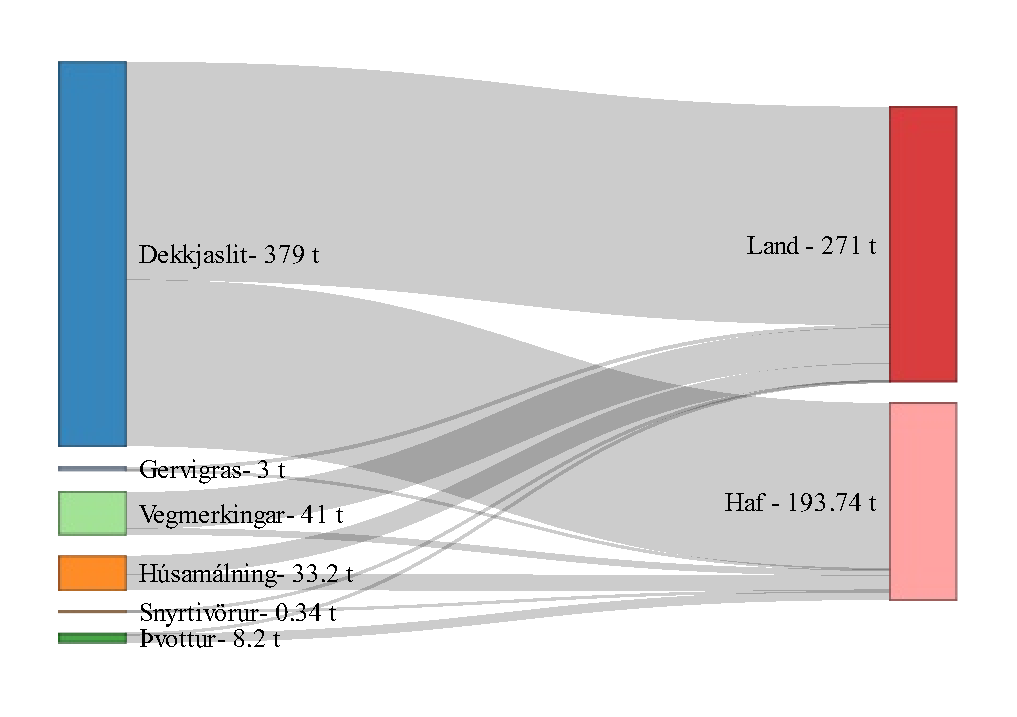
\includegraphics{OrplastHaf_files/figure-latex/unnamed-chunk-6-1} 

}

\caption{Helstu uppsprettur örplasts á Íslandi og skipting í haf eða í jarðveg. Byggt á lægra mati.}\label{fig:unnamed-chunk-6}
\end{figure}

\hypertarget{samgongur-byggingar-og-inaur}{%
\section*{Samgöngur, byggingar og iðnaður}\label{samgongur-byggingar-og-inaur}}
\addcontentsline{toc}{section}{Samgöngur, byggingar og iðnaður}

Stærstu uppsprettur örplasts á Íslandi eru frá umferð um malbikaða vegi. Hjólbarðar og vegamálning innihalda plast sem verður að örplasti við slit\textsuperscript{\protect\hyperlink{ref-kreider2010physical}{76}} en óvissa um afdrif þeirra er umtalsverð. Umferðarþungi hefur aukist síðasta áratuginn á Íslandi (yfir 20\% í Reykjavík og um 30\% á þjóðvegum \ref{fig:umferdvisitala1}). Umferð á Íslandi fer að langmestu leyti um malbikaða vegi í þéttbýli og eftir þjóðvegum landsins. Farleiðir dekkjaagna (dekkja- og vegaagna) af vegum til sjávar eru annars vegar með vindum og hins vegar með ofanvatni\footnote{„Uppbygging byggðar hefur þau áhrif að ógegndræpt yfirborð lands eykst, og vatn sem áður átti greiða leið ofan í jarðveg safnast saman á yfirborði ef ekkert er að gert. Úrkomuvatn sem fellur af húsþökum, götum, gangstéttum, bílastæðum og öðru þéttu yfirborði niður í fráveitukerfi er oft kallað „ofanvatn``. Hefðbundnar lausnir fela jafnan í sér að safna ofanvatni í fráveitukerfi sem er neðanjarðar, og leiða það þannig í pípum útaf svæðinu, oftast alla leið til sjávar.``\textsuperscript{\protect\hyperlink{ref-StefanFreyr}{77}}}.

Umferðarþungi hefur aukist síðasta áratuginn á Íslandi (\href{http://www.vegagerdin.is/upplysingar-og-utgafa/umferdin/tolfrumferdar/}{yfir 30\% í Reykjavík og um 45\% á þjóðvegum} sjá \ref{fig:umferdvisitala1}). Slit á hjólbörðum er ein af stærstu einstöku uppsprettum örplasts í heiminum\textsuperscript{\protect\hyperlink{ref-sundt2014sources}{32},\protect\hyperlink{ref-lassen2015microplastics}{78},\protect\hyperlink{ref-essel2015sources}{79}}. Frá því eftir miðbik síðustu aldar hafa stöðugar tækniframfarir verið drifnar áfram af pólitískum aðgerðum til að minnka mengun frá útblæstri bíla\textsuperscript{\protect\hyperlink{ref-lee2007innovation}{80}} en í seinni tíð hefur kastljósið í meira mæli beinst að mengun ótengdri útblæstri. Dekkjaagnir eru mikilvægur hluti af þeirri mengun þar sem milli 20\% og 50\% gúmmís í dekkjum farþegabíla fellur til á formi svifryks\footnote{Svifryk er venjulega skilgreint sem agnir smærri en 10 \(\mu\)m (PM\textsubscript{10}) en agnir minni en 10 μm í þvermál eru mögulega líffræðilega virkar þar sem þær komast ofan í lungun hjá fólki\textsuperscript{\protect\hyperlink{ref-heyder1986deposition}{81}}. Dekkjaagnir eru að jafnaði lítill hluti af svifryki frá vegum en þær hafa mælst frá 3\% til 7\% af rúmmáli í fínu svifryki (PM\textsubscript{2,5}) og allt að 10\% í grófara svifryki (PM\textsubscript{10})\textsuperscript{\protect\hyperlink{ref-grigoratos2014non}{82}}. Þó ber að nefna að í íslenskri rannsókn fundust ekki dekkjaagnir í svifryki í Reykjavík\textsuperscript{\protect\hyperlink{ref-Efla2015}{83}}. Aðstæður í Reykjavík eru sérstakar miðað við þá staði þar sem framkvæmdar eru þær rannsóknir á svifryki sem hér er vísað í. Í Reykjavík er meðalhiti lágur og mikill fjöldi rigningardaga en blautir vegir og lágt hitastig verja dekk sliti\textsuperscript{\protect\hyperlink{ref-le1998evaluation}{84}}.} og stærri agna þegar hjólbarðarnir eyðast við akstur\textsuperscript{\protect\hyperlink{ref-atech2001national}{85}}. Dekkjaagnir eru að mestum hluta stærri en svifryk\textsuperscript{\protect\hyperlink{ref-kreider2010physical}{76}} og setjast í kringum vegina\textsuperscript{\protect\hyperlink{ref-Cadle1978}{69}} og í malbikið sjálft en malbik er misgljúpt eftir notkun\textsuperscript{\protect\hyperlink{ref-Verschoor2016}{86}}. Uppsöfnun er þó takmörkuð þar sem vind hreyfir mikið og úrkoma skolar vegryki burtu með affallsvatni. Dekkjaagnir sem falla til geta brotnað niður að hluta við núninginn við vegina þegar þær losna frá dekkjunum sem veikir mótstöðu þeirra gagnvart útfjólubláu ljósi og færir þær nær niðurbroti í umhverfinu\textsuperscript{\protect\hyperlink{ref-Cadle1978}{69},\protect\hyperlink{ref-kreider2010physical}{76}}.

\begin{figure}

{\centering 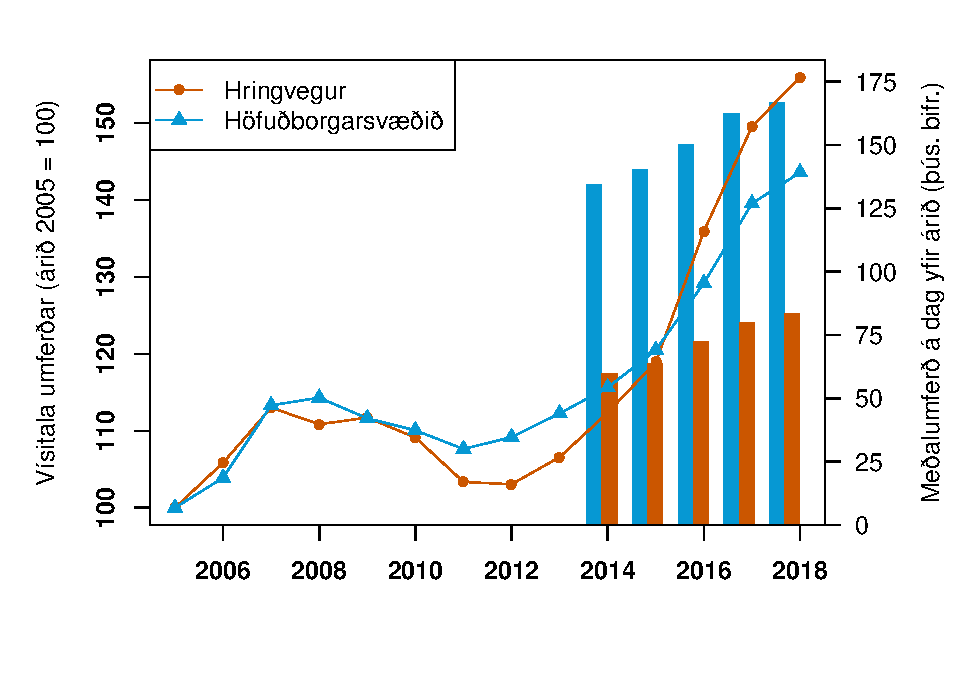
\includegraphics{OrplastHaf_files/figure-latex/umferdvisitala1-1} 

}

\caption{Vísitala umferðar (línur) ásamt meðalumferðarþunga yfir árið (stöplar) í þremur völdum sniðum innan höfuðborgarsvæðisins og á 16 lykilteljurum á hringveginum.}\label{fig:umferdvisitala1}
\end{figure}

Íslenskir vegir eru byggðir á fyllingu með gljúpum jarðvegi og greiðri afvötnun\textsuperscript{\protect\hyperlink{ref-Matinupa2012Summary}{87}} en þar sem plast er ekki vatnsleysanlegt gerum við ráð fyrir að það síist burtu út í jarðveginn frekar en að ferðast með grunnvatni\textsuperscript{\protect\hyperlink{ref-ECHA2016}{88}}. Ofanvatn rennur að mestu út í jarðveginn við vegina en í þéttbýli rennur það einnig í ræsi í eða í læki og ár. Á strjálbýlli svæðum taka vegrásir og skurðir við ofanvatni. Hérlendar byggðir eru flestar við ströndina og helstu vegir milli bæja liggja eftir strandlengjunni og er því ekki löng leið milli helstu vega og sjávar. Þær agnir sem ofanvatnið ber með sér festast því síður í jarðvegi og ferskvatnsseti við slíkar aðstæður en aukin fjarlægð eykur líkurnar á viðloðun í jarðvegi eða botnfellingu\textsuperscript{\protect\hyperlink{ref-BESSELING2017540}{89}}.

Það fer í stórum dráttum eftir þéttni byggðar hversu háu hlutfalli ofanvatns er veitt í hafið með fráveitukerfum eða hve mikið seytlar niður í jarðveginn (sjá mynd \ref{fig:ALTA})). Þar sem íslenskt þéttbýli er heldur í dreifðara lagi þá er hér reiknað með eftirfarandi:

\begin{itemize}
\tightlist
\item
  Á þjóðvegum og sveitavegum fari 90\% af affallsvatni vega í jarðveginn og 10\% í yfirborðsvatn; skurði, ár og læki\textsuperscript{\protect\hyperlink{ref-Verschoor2016}{86}}
\item
  Í þéttbýli hérlendis fari 40\% af affallsvatni vega í jarðveginn en 60\% í ræsi.\textsuperscript{\protect\hyperlink{ref-Verschoor2016}{86}}
\end{itemize}

\begin{figure}

{\centering 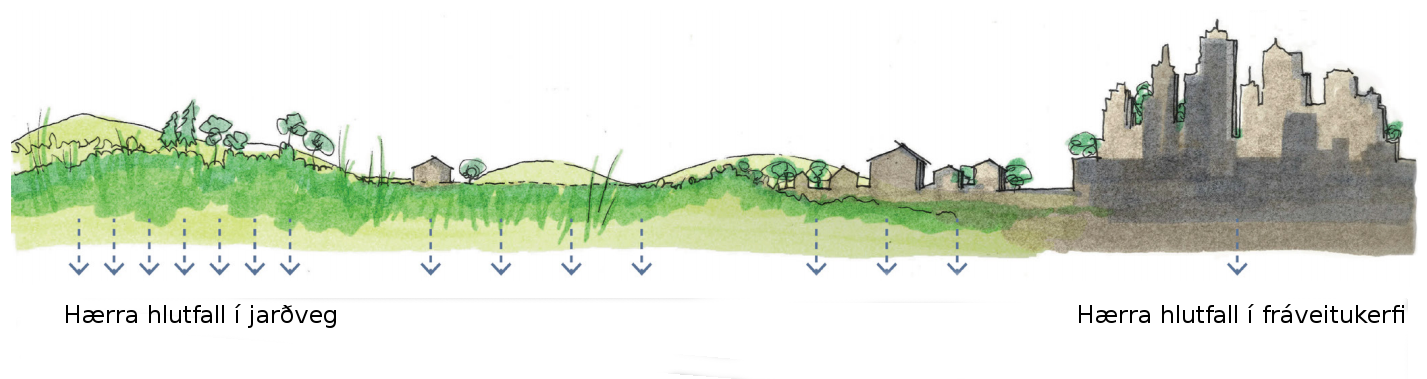
\includegraphics[width=1\linewidth]{myndir/ALTA} 

}

\caption{Myndin sýnir í stórum dráttum hlutfall ofanvatns sem rennur í jarðveg á móti hlutfalli ofanvatns sem rennur í hefðbundið fráveitukerfi miðað við þéttleika byggðar. Mynd fengin frá Alta (2016)}\label{fig:ALTA}
\end{figure}

Við metum það sem svo að affallsvatn sem lendir í fráveitukerfum beri allar dekkjaagnir sem það inniheldur út í haf en það affallsvatn sem rennur í jarðveg losni við allar dekkjaagnir í jarðveginn. Það skal þó tekið fram að aðstæður eru mjög ólíkar á mismunandi svæðum landsins bæði m.t.t. jarðvegsgerðar og einnig eiginleika þéttbýla og þar stendur Reykjavík út úr. Mælingar á dekkjaögnum í affallsvatni eru erfiðar í framkvæmd og gögn skortir. Nokkur líkön hafa verið gerð til að áætla magn örplasts í framburði stórra áa í Evrópu en þau eru sum hver í mótsögn hvor við aðra\textsuperscript{\protect\hyperlink{ref-unice2019characterizing1}{65}}. Þau eiga það þó sameiginlegt að áætla örplast frá dekkjum heilli stærðargráðu lægra en í þessari skýrslu þar sem þau lýsa aðstæðum sem eru gjörólíkar íslenskum aðstæðum t.d. er fjarlægð helstu uppspretta örplsts (borgir) í tugum til hundruða kílómetra fjarlægð frá árósum.

\hypertarget{hjolbarar-bifreia}{%
\subsection*{Hjólbarðar bifreiða}\label{hjolbarar-bifreia}}
\addcontentsline{toc}{subsection}{Hjólbarðar bifreiða}

Hjólbarðar eyðast smám saman við akstur vegna núnings við vegi. Margir þættir hafa áhrif á slit hjólbarða en það er mismikið eftir gerð dekkja, stærð bíla og aksturslagi\textsuperscript{\protect\hyperlink{ref-panko2018review}{90}}. Þar sem fleiri beygjur eru á vegum og hröðunarbreytingar eru tíðari verður meira álag á dekkin og slit á þeim verður meira. Því er eyðing dekkja minni á þjóðvegum en vegum í þéttbýli\textsuperscript{\protect\hyperlink{ref-luhana2004measurement}{91},\protect\hyperlink{ref-Kwak2013}{92}}.

Hjólbarðar eru samsettir úr flókinni blöndu efna sem er blandað með ólíkum hætti eftir þörfum. Slit er misjafnt eftir því fyrir hvaða gerð farartækja dekkin eru framleidd og hvernig slitlag vegarins er\textsuperscript{\protect\hyperlink{ref-grigoratos2014non}{82}}. Gúmmísólar venjulegra bíldekkja eru gerðir úr blöndu af gervigúmmíi (aðallega stýren bútadíen gúmmí og bútadíen gúmmí), náttúrulegu gúmmíi, kinroki (e. carbon black) og ýmsum íblöndunarefnum\textsuperscript{\protect\hyperlink{ref-Evans2006}{93}}. Hlutfall plastfjölliða í slitlagi hjólbarða er á bilinu 40-60\%\textsuperscript{\protect\hyperlink{ref-Redondo-hasselerharm2018}{94}--\protect\hyperlink{ref-barbin1994science}{96}} (tekið saman af\textsuperscript{\protect\hyperlink{ref-Wik2009}{97}}). Dekkjaagnirnar sem myndast við akstur blandast öðrum ögnum sem eru í malbikinu og vegrykinu sem breytir efnasamsetningu agnanna\textsuperscript{\protect\hyperlink{ref-kreider2010physical}{76}}. Þessi blanda dekkja- og vegslits (e. tyre and road wear particles - TRWP) getur því til viðbótar innihaldið efni á borð við bik, þ.e. úr malbiki\textsuperscript{\protect\hyperlink{ref-fauser2002tire}{98}}, og ryk frá bremsuborðum/diskum\textsuperscript{\protect\hyperlink{ref-kwak2013characterization}{99}}. Í þessari skýrslu er litið á gúmmíblönduna, ásamt öðrum bætiefnum sem er er blandað saman í slitlagi hjólbarða, sem eina heild óháð fjölliðuinnihaldi.

Ein leið til að áætla magn dekkjaslits er að miða við staðlaðar losunartölur mg/km ólíkra þyngdarflokka ökutækja. Samkvæmt Klein (2017)\textsuperscript{\protect\hyperlink{ref-klein2017methods}{100}} er slit hjólbarða fólksbifreiða 85-132 milligrömm fyrir hvern ekinn kílómetra, hópbifreiða 267-415 mg/km, sendibifreiða 102-159 mg/km og vörubifreiða 546-850 mg/km.

Í töflu \ref{tab:akstur} má sjá fjölda bifreiða af mismunandi gerðum í umferð á Íslandi (þann 14. ágúst 2018) og meðalakstur samkvæmt upplýsingum frá Samgöngu- og sveitarstjórnaráðuneytinu. Séu þessar tölur margfaldað með áætluðu dekkjasliti fyrir viðkomandi ökutækjaflokka \emph{i} er áætlað dekkjaslit er reiknað á eftirfarandi hátt: Losun\textsubscript{i} = (fjöldi × meðalakstur × mg/km)\textsubscript{i}. Niðurstaðan er þá að árið 2017 hafi slit frá fólksbifreiðum verið 244-378 tonn, sendibifreiðum 34-52 tonn, hópbifreiðum 22-34 tonn, og vörubifreiðum 79-122 tonn.

Farleiðir dekkjaslits er að langmestu leiti með affallsvatni vega\textsuperscript{\protect\hyperlink{ref-Verschoor2016}{86}} og eru vindbornar agnir svotil utanskildar í þessari skýrslu. Losun örplasts vegna dekkjaslits er áætlað. Við metum það sem svo að:

\begin{itemize}
\tightlist
\item
  um þriðjungur allrar umferðar sé á hringvegi þar sem hverfandi magn dekkjaslits berst til hafs.
\item
  um 2/3 hlutar allrar umferðar sé í þéttbýli þar sem hátt hlutfall dekkjaslits berst til hafs eða um 60\% í gegnum ræsi.
\end{itemize}

Áætluð heildarlosun örplasts í hafið frá sliti bifreiðahjólbarða á Íslandi er \textbf{164-255} tonn.

\begin{table}[t]

\caption{\label{tab:akstur}Áætluð árleg losun örplasts í hafið vegna slits á hjólbörðum bifreiða. Fjöldi bíla af mismunandi gerðum í umferð á Íslandi þann 14. ágúst 2018 og meðalakstur skv. Umferðastofu. Með meðalþyngd er átt við heildarþyngd skv. reglugerð. Byggt á mati Klein (2017) og Verschoor (2016)}
\centering
\begin{tabular}{lllll}
\toprule
  & Fólksbifreið & Sendibifreið & Hópbifreið & Vörubifreið\\
\midrule
Fjöldi & 227409 & 23159 & 2410 & 8078\\
Meðalþyngd (t) & 2,05 & 2,66 & 9,75 & 17,18\\
Meðalakstur (þús. km/ár) & 12,6 & 14,25 & 33,69 & 17,83\\
Slit (mg/km) & 85-132 & 102-159 & 267-415 & 546-850\\
Slit (t/ár) & 244-378 & 34-52 & 22-34 & 79-122\\
\addlinespace
Losun í hafið (t/ár) & 97-151 & 13-21 & 9-13 & 31-49\\
\bottomrule
\end{tabular}
\end{table}

\begin{figure}

{\centering 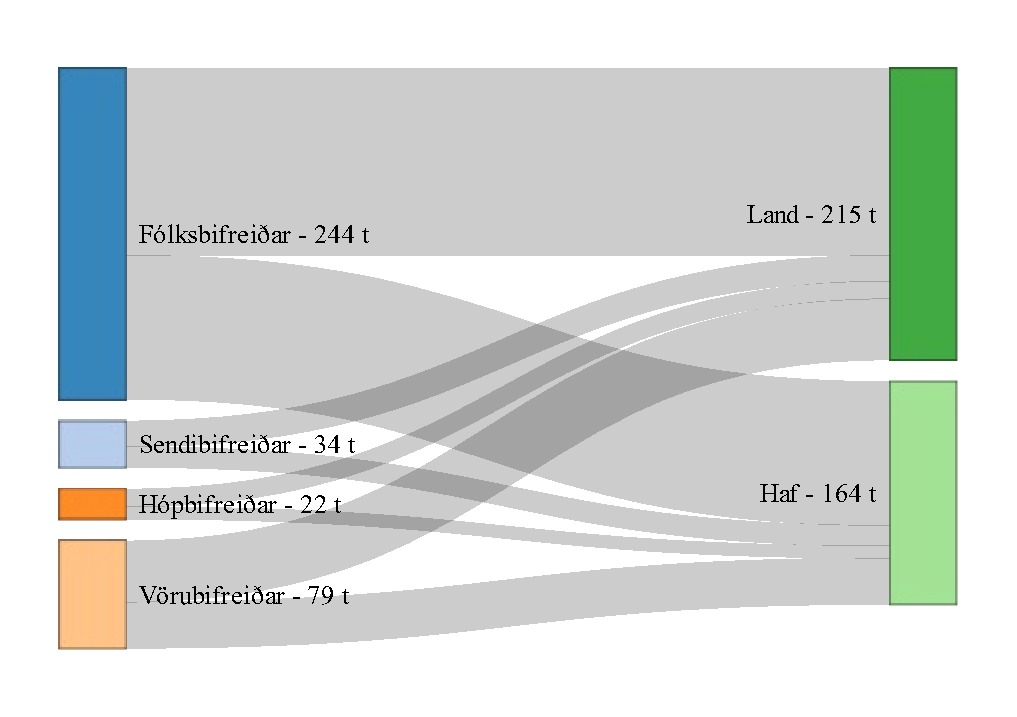
\includegraphics{OrplastHaf_files/figure-latex/akstur2-1} 

}

\caption{Losun örplasts frá hjólbörðum á land og í haf skv. lægra mati}\label{fig:akstur2}
\end{figure}

\hypertarget{vegmerkingar}{%
\subsection*{Vegmerkingar}\label{vegmerkingar}}
\addcontentsline{toc}{subsection}{Vegmerkingar}

Samkvæmt upplýsingum frá Vegagerðinni er á Íslandi notast við þrenns konar vegmerkingar og innihalda þær allar plastefni: málningu, sprautuplast og vélmössun. Slitþol þeirra er mismunandi en málning þolir minnst og vélmössun mest. Málaðar vegmerkingar eru 0,2-0,3 mm að þykkt, sprautuplast 0,7-1,5 mm og vélmössun 3,0 mm.

Sprautuplastefni er mest notað til vegmerkinga en það er flutt inn til landsins á duftformi sem er brætt á staðnum við merkingar og lagt á vegina. Þegar efnið er hitað rennur það og er hægt að mála með því miðlínur vega, kantlínur, gangbrautir og fleira en svo harðnar það fljótt. Settar eru glerperlur í blautt efnið til að fá endurskin. Hvítur litur fæst með títaníum díoxíði (TiO\textsubscript{2}).

Sundrun plastefna í vegmerkingum vegna útfjólublárrar geislunar hefur ekki verið rannsakað en miðað við utanhússmálningu gerum við ráð fyrir að það hún sé umtalsvert minni þar sem líftími vegmerkinga er aðeins um eitt ár.

Veðurfarsþættir á borð við úrkomu, vind og hitastigsbreytingar (einkum í kringum frostmark) valda augljóslega einhverju sliti og molnun yfirborðsmerkinga en helstu áhrifaþættirnir eru umferð ökutækja og snjótennur snjómokstursbíla. Áhrif umferðar eru háð fjölda ekinna kílómetra um vegina en vert er að gefa gaum áhrifum snjómoksturs.

Vegna skiljanlegra krafa um að vegir séu vel hreinsaðir af snjó er nokkuð algengt að snjótennur skrapi vegmerkingar af vegum og jafnvel hluta af slitlaginu sjálfu. Á þetta einkum við þegar hjólför hafa myndast og vegir eru ójafnir en aðferðir við snjómokstur geta einnig haft áhrif. Þó að almenn umferð sé helsta orsök slits vegmerkinga er giskað á að slit af völdum snjómoksturs sé mögulega allt að 15\% þótt hafa beri í huga að mælingar hafa ekki verið gerðar (pers. heimild Vegagerðin). Snjómokstur hefur reynst vera mikilvægur farvegur fyrir vegmerkingar og fleiri gerðir plastefna út í hafið á svæðum þar sem snjó er ýtt út í sjó\textsuperscript{\protect\hyperlink{ref-BaztanJ2018}{101}}.

Misjafnt er eftir heimildum hvernig losun örplasts frá vegmerkingum er metið. Í norskri skýrslu\textsuperscript{\protect\hyperlink{ref-sundt2014sources}{32}} er talað um að allar vegmerkingar sem notaðar séu árlega reiknist með sem losun örplasts vegna slits. Í danskri skýrslu\textsuperscript{\protect\hyperlink{ref-lassen2015microplastics}{78}} er ekki reiknað með þeim vegmerkingum sem áætlað er að fari á nýtt malbik og að um 15-25\% fari í endurlagningu en í þýskri rannsókn\textsuperscript{\protect\hyperlink{ref-Commission2009}{102}} er talað um að um að þetta hlutfall sé 80\%. Samkvæmt sérfræðingum Vegagerðarinnar er um 87\% vegmerkinga hérlendis vegna slits og er því tekið með í reikninginn sem uppspretta örplasts.

Vegmerkingum á Íslandi er skipt á milli Vegagerðarinnar og sveitarfélaganna. Vegagerðin sér um þjóðvegina sem liggja um landið og í gegnum flesta þéttbýlisstaði, til dæmis liggja nokkrir vegir Vegagerðarinnar í gegnum Reykjavík og svo liggja þeir gjarnan niður á höfn í gegnum minni bæi úti á landi. Unnt er að áætla slit vegmerkinga Vegagerðarinnar út frá því magni sem bætt er á vegi hennar á landsvísu ár hvert.

Árið 2017 notaði Vegagerðin 155.000 L (1,65 g/L ≈ 250 t) af vegmálningu, 454 t af sprautuplasti og 182 t af vélmössun (\href{https://www.geveko-markings.com/fileadmin/root/msds/Thermoplastics/ViaTherm/MSDS_ViaTherm_hydrocarbon_EN-GB.pdf}{sama efnið notað}). Sé miðað við óstaðfestar upplýsingar frá framleiðanda er fjölliðuinnihald sprautuplastsins frá 1 til 8\% en í málningunni er innihald akrýlfjölliða á bilinu 15-40\% skv.(\href{\%22/skjol/Mercalin\%20AQ\%20white\%206010\%20vatnsmálning\%20CLEANOSOL-3.pdf\%22}{öryggisleiðbeiningum})

Nauðsynlegt er að endurnýja vegmerkingar sem sjást illa en umfang þeirra er nokkuð stöðugt milli ára hjá Vegagerðinni þar flestar miðlínur á íslenskum þjóðvegum eru endurlagðar árlega sem er ólíkt því sem gerist í nálægum samanburðarlöndum. Í Bretlandi er reynt að fara eftir vissum staðli um sýnileika og ekki málað fyrr en vegmerkingar eru umtalsvert eyddar (30\% í þéttbýli en 70\% á þjóðvegum)\textsuperscript{\protect\hyperlink{ref-Hann2018}{103}}. Miðað við útboðsgögn nokkurra stórra sveitarfélaga er notkun sprautuplasts um 0,6 kg á mann á ári í stærri þéttbýlum. Í minni þéttbýlum er algengt að notuð sé málning frekar en plast og í minna magni\footnote{Á Ísafirði, Bolungarvík, Sauðárkróki, Fjallabyggð, Skagaströnd, Dalvík er málað en í Hveragerði er massað. Skv. Gauti Ívari Halldórssyni framkvæmdastjóra \href{http://www.bilastaedamalun.is/}{vegmerkingafyrirtækis} sem sér um vegmerkingar á þessum stöðum (nema Skagaströnd) er málað frekar en massað í flestum minni þéttbýlum}. Þar er algengt að um 0,2 kg á mann sé notað af vegamálningu sé notuð árlega. Miðað við forsendur sem tilteknar eru í töflu \ref{tab:vegmerkingar} má áætla að á Íslandi sé árleg uppspretta örplasts vegna slits á vegmerkingum sé 41-256 t.

\begin{table}[t]

\caption{\label{tab:vegmerkingar}Áætluð árleg uppspretta örplasts frá vegmerkingum á Íslandi árið 2017}
\centering
\begin{tabular}{ccccccccc}
\toprule
 &  &  & kg/mann &  & Tonn & \% & Tonn & Tonn\\
\midrule
Stærri sveitarfélög & Sprautuplast & 254.280 & 0,6 & 87\% & 110 & 1-25 & 1-28 & 0,6-16,8\\
Minni sveitarfélög & Málning & 84.170 & 0,2 & 87\% & 15 & 15-40 & 2-6 & 1,3-3,6\\
Vegagerðin & Sprautuplast &  &  & 87\% & 543 & 1-25 & 5-135 & 0,5-13,5\\
Vegagerðin & Málning &  &  & 87\% & 218 & 15-40 & 33-87 & 3,3-8,7\\
\bottomrule
\end{tabular}
\end{table}

Líkt og við á um dekkjaagnir berst slit frá vegmerkingum helst með vindi og ofanvatni í jarðveg eða fráveitukerfi, skurði, ár og læki. Miðað við 60\% ofanvatns berist í fráveitukerfi í þéttbýli og 10\% í dreifbýli má áætla að losun örplasts í hafið frá vegmerkingum sé \textbf{5,7 - 42,6}.

\begin{figure}
\centering
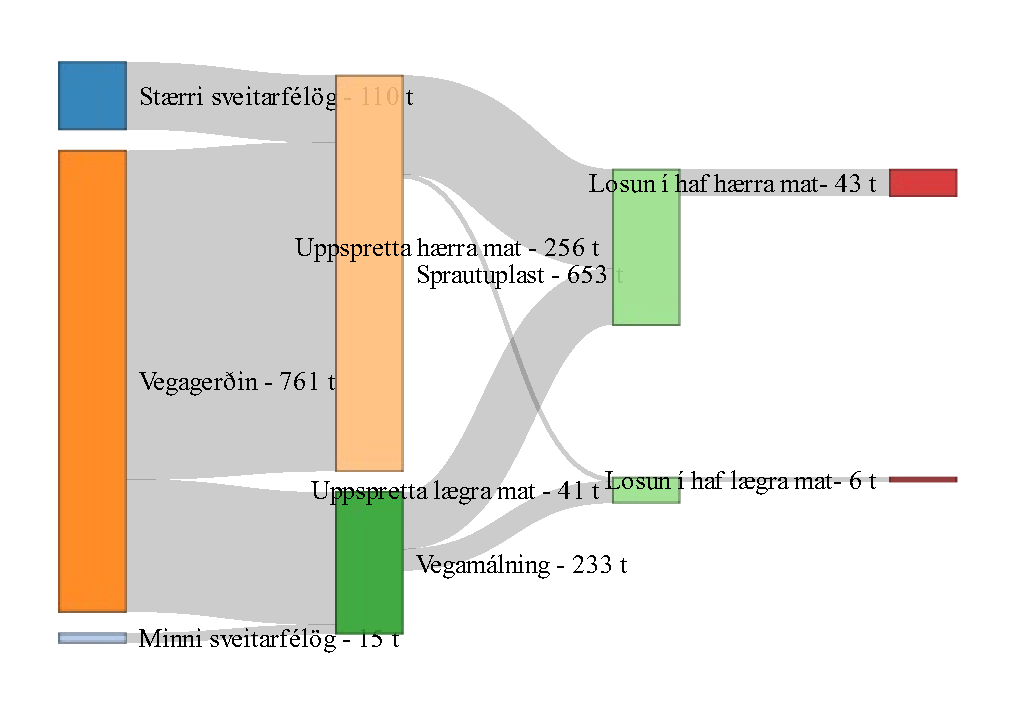
\includegraphics{OrplastHaf_files/figure-latex/vegmerkingar2-1.pdf}
\caption{\label{fig:vegmerkingar2}Áætluð árleg heildarlosun örplasts í hafið frá vegmerkingum á Íslandi árið 2017 er \textbf{5,7 - 42,6 t}.}
\end{figure}

\hypertarget{hjolbarar-flugvela}{%
\subsubsection*{Hjólbarðar flugvéla}\label{hjolbarar-flugvela}}
\addcontentsline{toc}{subsubsection}{Hjólbarðar flugvéla}

Ólíkt hjólbörðum ökutækja eru hjólbarðar flugvéla einungis notaðir við upphaf og lok ferðalags og slit þar af leiðandi hlutfallslega minna og einskorðað við flugvelli. Hér er gert ráð fyrir að hjólbarðar flugvéla séu gerðir úr gúmmíblöndu sem er ekki það frábrugðin hinum ýmsu samsetningum annarra hjólbarða að það breyti nokkru fyrir tilgang þessarar skýrslu.

Ein leið til að áætla losun örplasts frá hjólbörðum flugvéla er að margfalda fjölda flughreyfinga, þá er átt við flugtak og lendingu saman, með áætluðu dekkjasliti. Hér er gerður greinarmunur á millilandaflugi og innanlandsflugi þar sem stærri flugvélar eru alla jafna notaðar í millilandaflugi.

Dæmigerðar millilandaflugvélar eru flugvélar á borð við Boeing 757\textsuperscript{\protect\hyperlink{ref-kole2017wear}{104}} og Airbus 321 (pers. heimild) sem vega frá 30 til 65 tonna án farþega og eru með fjögur til átta aðalhjól og tvö framhjól. Slit hjólbarða flugvéla í hverri flughreyfingu (tekið saman af Kole\textsuperscript{\protect\hyperlink{ref-kole2017wear}{104}}) er metið um 21 gramm frá hverju framhjóli og 59 grömm frá hverju aðalhjóli eða 278-514 grömm í heildina. Sé áætlað dekkjaslit margfaldað með fjölda flughreyfinga í millilandaflugi á Íslandi árið 2017 (65.528 flughreyfingar)\textsuperscript{\protect\hyperlink{ref-isavia2017}{105}} nemur það 18 til 34 tonnum af dekkjasliti árlega.

Flugvélar í innanlandsflugi á Íslandi eru flestar á bilinu 10 til 18 tonn án farþega (t.d. Bombardier Q400 (18 tonn), Bombardier Q200 (10 tonn) og Jetstream 32 (10 tonn)). Ekki fundust tölur um slit hjólbarða hjá þessum flugvélum en sé lauslega gert ráð fyrir að slitið sé í kringum 1/3 af því sem áætlað er fyrir flugvélar í millilandaflugi. Af hinum tæpu 130 þúsund flughreyfingum hérlendis árið 2017 voru 75 þúsund þeirra snertilendingar sem reiknast sem 0,5 flughreyfing. Með sömu aðferðum og notaðar voru við að meta dekkjaslit frá millilandaflugi má áætla um 8-16 tonnum árlega vegna innanlandsflugs. Árlegt magn dekkjaslits frá hjólbörðum flugvéla er því metið 26-50 tonn. Þetta mat er byggt er á óáreiðanlegum forsendum og ekki var unnt notast við nákvæma stærðarflokkun þeirra flugvéla sem lentu og tóku á loft á Íslandi og því viðbúið að skekkja matsins sé talsverð.

Allar flugbrautir á Keflavíkurflugvelli afvatnast út í jarðveginn í kring og berst því líklega ekki í hafið í miklu mæli. Fráveitukerfi flugvallarins tekur við ofanvatni frá byggingum á vellinum. Ekki var kannað hvernig fráveitumálum er háttað við aðra flugvelli eru staðsettir við sjó eða við fljót í tilfelli Egilstaðaflugvallar. Ekki er hægt að meta losun örplasts í hafið frá flugvélahjólbörðum hérlendis að svo stöddu en uppspretta örplasts frá hjólbörðum flugvéla í umhverfið árlega er \textbf{26-50 tonn}.

\hypertarget{malning}{%
\section*{Málning}\label{malning}}
\addcontentsline{toc}{section}{Málning}

\emph{Fyrirvari: Innlend framleiðsla er ekki tekin með í reikninginn hér því ekki fengust nákvæmar upplýsingar um innflutt magn þeirra efna sem eru notuð til að blanda málningu. Hægt er að nálgast lista yfir fyrirtæki sem kaupa inn vissar vörur og grennslast betur fyrir um hvaða efni um ræðir en Tollstjóri má ekki afhenda þann lista nema með lagaheimild.}

Málnin sem er hellt niður í ræsi er aðeins solid content af örplasti en málningarflögur eru 100\% örplast

\hypertarget{utanhussmalning}{%
\subsection*{Utanhússmálning}\label{utanhussmalning}}
\addcontentsline{toc}{subsection}{Utanhússmálning}

Flestar gerðir málningar eru með syntetískum fjölliðum sem bindiefni\textsuperscript{\protect\hyperlink{ref-Durkin2018}{106}} og vitað er að málning slitnar og veðrast. Mest er innflutt af akrýl- og vínylblandaðri málningu til landsins til notkunar innanhúss og utan en bæði þessi efni eru plastefni. Utanhússmálning flagnar af og veðrast að einhverju leyti en aðallega losnar hún af við háþrýstiþvott og getur borist til hafs með fráveitukerfum og vindum. Það skal tekið fram að hluti plastefna í utanhússmálningu sundrast vegna útfjólublárrar geislunar og vatnsrofs og berst því ekki í umhverfið sem örplast. Á líftíma málningar á veggjum og þökum utanhúss brotnar allt að 67\% einliða plastefnanna niður í koltvísýring, vatn og nitur\textsuperscript{\protect\hyperlink{ref-Hann2018}{103}} og er sá hluti því dreginn frá heildarlosun örplasts frá utanhússmálningu.

Markaðshlutur innimálningar gagnvart útimálningu er ólíkur milli rannsókna í mismunandi löndum. Í Danmörku og Svíþjóð var útimálning metin 63\% af heildarmagni en aðeins 27\% í Evrópusambandsríkjunum\textsuperscript{\protect\hyperlink{ref-Hann2018}{103}}. Í norsku örplastsskýrslunni má umreikna að þar sé hlutfallið um 35\%\textsuperscript{\protect\hyperlink{ref-sundt2014sources}{32}}. Munurinn á milli norðurlandanna og Evrópusambandsríkjanna getur skýrst af því að meiri veðrun í norðlægari byggðum krefjist meiri útimálningar\textsuperscript{\protect\hyperlink{ref-Hann2018}{103}} en ólík menning spilar einnig inn í. Á Íslandi er veðrun útimálningar einnig mikið vandamál sem rökstyður samanburð við hin Norðurlöndin en hér er bygginarstíll þó um margt ólíkur þeim.

Timburklædd hús þarf að mála oftar en steinhús. Á Íslandi er lítið um timburklædd hús en hér eru aftur á móti nánast engar ómálaðar múrsteinsbyggingar sem eru mjög algengar í Skandinavíu og víðar Evrópu. Þrátt fyrir þónokkurn fjölda steinaðra bygginga hér á landi (um 3000 byggingar um síðustu aldamót) sem ætti ekki að þurfa að mála\textsuperscript{\protect\hyperlink{ref-Guuxf0mundsson2003}{107}} eru flest hús máluð og ólíkt nágrannaþjóðunum mála Íslendingar næstum öll þök.

Útimálun er framkvæmd vegna nýbygginga eða slits, bæði á þökum og veggjum en innimálun er hins vegar framkvæmd við eigendaskipti og nýbyggingu. Hlutfall sölu útimálningar hjá innlendum söluaðilum er mishátt eftir því hvort viðskiptin eru við fagmenn eða heimili.
Samkvæmt tölvupósti er hlutfall útimálningar undir 30\% hjá stórum söluaðila sem afgreiðir heimili að mestu en hærra hjá öðrum stórum söluaðila (yfir 60\%) sem afgreiðir að mestu fagmenn.

Innflutt málning árin 2016 og 2017 var 3.15 þúsund tonn á ári\textsuperscript{\protect\hyperlink{ref-tollur2017}{108}} eða um 9,3 kg á mann (hér er ekki tekið með efni sem notuð eru til framleiðslu á málningu hérlendis). Þetta er af sömu stærðargráðu og mat Hann\textsuperscript{\protect\hyperlink{ref-Hann2018}{103}} um málningarnotkun á mann í Evrópusambandsríkjunum (um 8,2 kg).

Losun örplasts frá utanhússmálningu hefur ekki verið könnuð beint og er þetta mat því aðeins byggt á fræðilegum grunni. Veðrun og slit málningar veldur losun á syntetískum fjölliðum út í umhverfið þar sem þær verða fyrir útfjólublárri geislun og geta brotnað niður að miklu leyti. Miðað við eftirfarandi forsendur má áætla örplastmengun frá útimálningu með eftirfarandi hætti:

\begin{itemize}
\tightlist
\item
  frá 27-63\% innfluttrar málningar séu notuð á fleti utanhúss (pers. heimildir)
\item
  að um 20\% af innihaldi málningar séu plastefni\textsuperscript{\protect\hyperlink{ref-Hann2018}{103}}
\item
  að 67\% plastefnanna sundrist vegna veðrunar (og reiknist því ekki með)\textsuperscript{\protect\hyperlink{ref-Hann2018}{103}}
\item
  að um 1.6\% utanhússmálningar flagni af (vegna veðrunar eða háþrýstiþvottar) sem örplast\textsuperscript{\protect\hyperlink{ref-Hann2018}{103}}
\item
  að um 2.5\% af eftirstandandi málningu losni sem örplast vegna veðrunar\textsuperscript{\protect\hyperlink{ref-Hann2018}{103}}
\end{itemize}

\begin{table}[t]

\caption{\label{tab:malningartafla}Uppspretta örplasts í umhverfið frá útimálningu á Íslandi.}
\centering
\begin{tabular}{ccc}
\toprule
Innflutt málning & Tonn & 3150\\
Hlutur utanhúss-málningar & \% & 27-63\\
 & Tonn & 850-2000\\
Plastefni & \% & 20\\
Sundrun & \% & 67\\
\addlinespace
Eftirstandandi & Tonn & 740-1720\\
Háþrýsti-þvottur & \% & 1,6\\
 & Tonn & 11,8-27,5\\
Uppspretta vegna slits & \% & 2,5\\
 & Tonn & 18,2-41,2\\
\bottomrule
\end{tabular}
\end{table}

Áætluð uppspretta örplasts frá utanhússmálningu á ári er því um 30-70 tonn. Þar sem um 70\% af flatarmáli bygginga er innan þéttbýlis\footnote{hér er þéttbýli skilgreint eftir gagnalaginu mannvirki í IS 50V kortagrunninum frá landhelgisgæslunni} er aftur farið eftir áætluðu hlutfalli ofanvatns sem rennur í ræsi (60\%)\textsuperscript{\protect\hyperlink{ref-Verschoor2016}{86}}. Byggingar utan þéttbýlis þar sem fráveita er nánast engin eru ekki hafðar með. Áætluð losun örplasts í hafið frá útimálningu er því \textbf{12-29 t}

\hypertarget{innimalning}{%
\subsection*{Innimálning}\label{innimalning}}
\addcontentsline{toc}{subsection}{Innimálning}

Örplastmengun vegna málningar innandyra verður aðallega vegna þrifa á penslum. Sú málning berst beint í hafið um fráveitukerfi og er reiknað með að hún sé um 1,6 \%\textsuperscript{\protect\hyperlink{ref-Hann2018}{103}}. Innimálning verður ekki fyrir mikilli veðrun og hvert lag er málað yfir það sem fyrir var án þess að það sé þvegið af.

\begin{table}[t]

\caption{\label{tab:innimalningartafla}Áætluð árleg losun örplasts í hafið frá innanhússmálningu á Íslandi.}
\centering
\begin{tabular}{ccc}
\toprule
Innflutt málning & Tonn & 3150\\
Hlutur innanhúss-málningar & \% & 37-73\\
 & Tonn & 1165-2300\\
Plastefni & \% & 20\\
 & Tonn & 230-460\\
\addlinespace
Ónýtt málning & \% & 3-15\\
Losun vegna skolunar & Tonn & 3,2-7,1\\
\bottomrule
\end{tabular}
\end{table}

Efmiðað er við að um 20\% af innihaldi málningar sé syntetískar fjölliður\textsuperscript{\protect\hyperlink{ref-Hann2018}{103}} er áætluð heildarlosun örplasts frá innimálningu á ári því \textbf{3,2-7,1} tonn.

Ekki er öll málning með plastbindiefnum því einnig eru alkýðbindiefni algeng í málningu sem eru með vatnssækna eiginleika og brotna á annan veg niður í náttúrunni. Mat á þrifum á verkfærum er byggt á lítilli þekkingu um vinnubrögð fagmanna (eru verkfæri skoluð, þeim hent). Nauðsynlegt er að gera markaðsrannsókn þar sem kannað er hve mikill hluti málningar er seldur til fagmanna og heimila. Einnig er nauðsynlegt að greinarmunur sé gerður á ólíkum bindiefnum í málningu og kannað verði til hlítar hve mikið af syntetískum fjölliðum til framleiðslu málningar er flutt inn í gegnum Tollstjóra.

\begin{figure}

{\centering 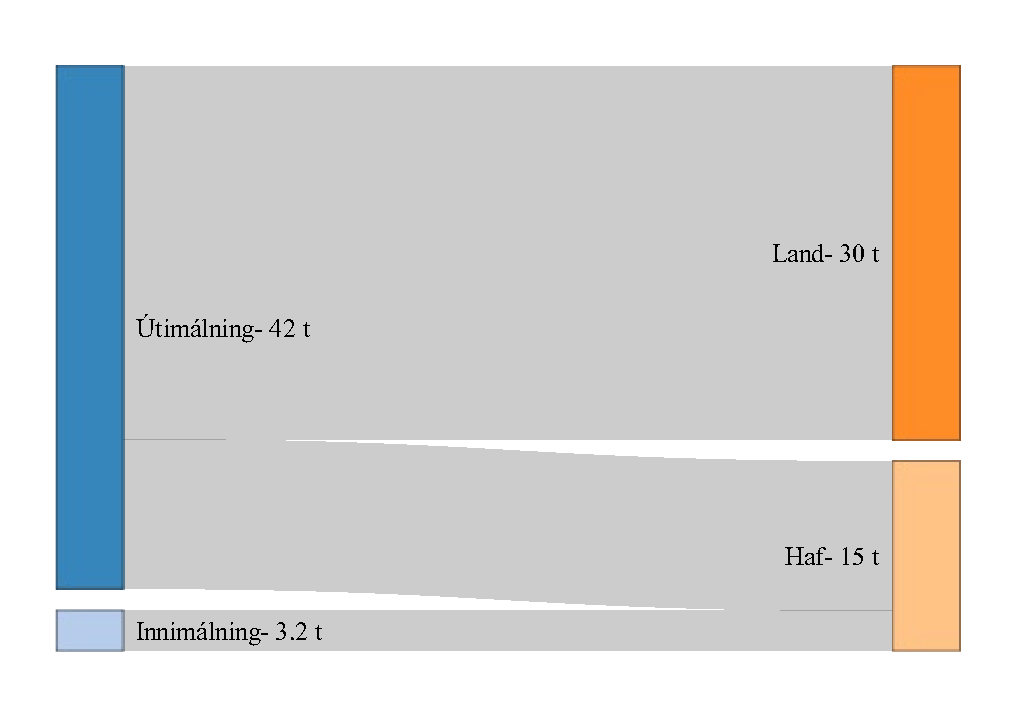
\includegraphics{OrplastHaf_files/figure-latex/unnamed-chunk-8-1} 

}

\caption{Áætluð árleg heildarlosun örplasts frá húsamálningu er 15,2-36,1 tonn}\label{fig:unnamed-chunk-8}
\end{figure}

\hypertarget{skipamalning}{%
\subsection*{Skipamálning}\label{skipamalning}}
\addcontentsline{toc}{subsection}{Skipamálning}

Í þessari skýrslu er sú nálgun valin að áætla magn skipamálningar út frá fjölda og stærð skipa. Skip eru með marga málaða fleti sem erfitt er að henda reiður á og því er hér aðeins stikað á stóru en til frekari einföldunar verða aðeins fiskiskip könnuð þar sem önnur skip eru mjög lítill hluti af skipaflota landsins. Ekki hefur verið framkvæmd markaðskönnun hjá söluaðilum til að meta magn skipamálningar frekar en annarrar málningar.

Fjórir stórir slippir eru á landinu, þar af þrír á SV-landi og einn á Akureyri. Minni slippir, eða dráttarbrautir sem geta tekið inn smærri báta, eru hér og þar um landið. Í slippum landsins eru nokkrir tugir skipa þjónustaðir árlega. Hver sem fær þjónustu hjá slippum getur haft sína hentisemi varðandi þykkt málningarlagsins og gerð málningar og sumir skaffa málningu sjálfir en aðrir kaupa af slippunum. Í stóru slippunum eru skip sprautumáluð en langflestir minni bátar eru málaðir með rúllum og penslum af eigendum þeirra. Þeir eru oft hífðir upp og málaðir nálægt bryggju. Mörg íslensk skip eru máluð í útlöndum og hérlendir slippir taka erlend skip á móti.

\begin{figure}

{\centering 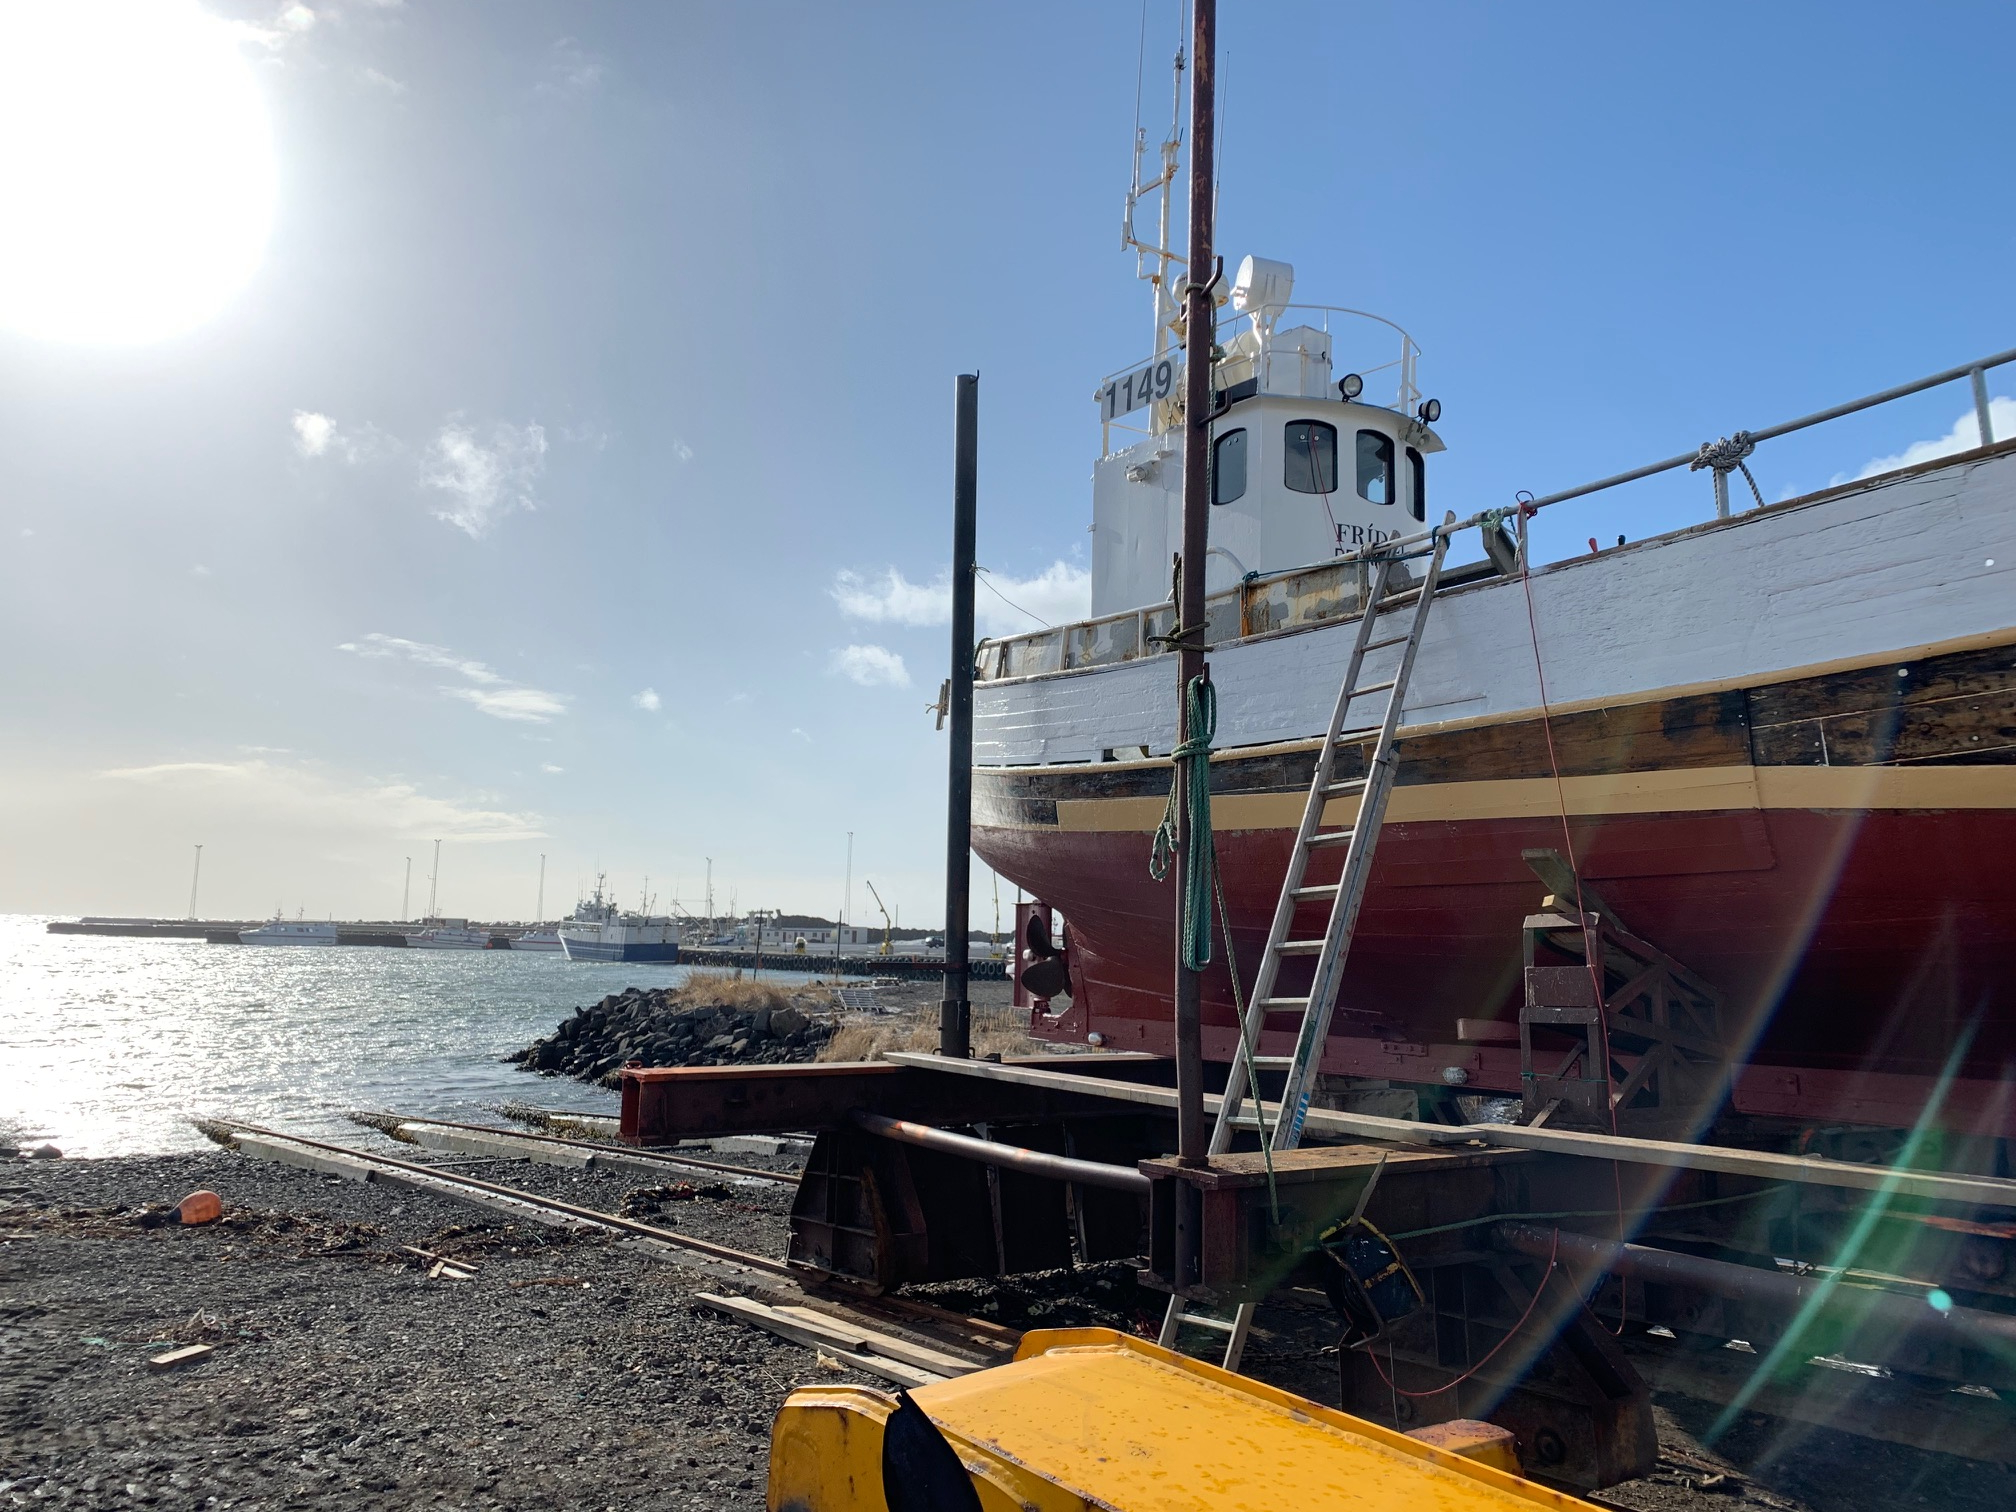
\includegraphics[width=0.6\linewidth]{myndir/slippur} 

}

\caption{Skip í slipp á Skagaströnd. Nokkrar smærri dráttarbrautir eru hér og þar um landið sem þjónusta eigendur smárra til meðalstórra skipa}\label{fig:Slippur}
\end{figure}

Málun er tíðust á botninum undir vatnslínunni og á þann flöt er notuð sérstök málning til varnar ásætum sem annars myndu auka viðnám skipsskrokksins. Skip eru máluð um það bil einu sinni á þriggja til fimm ára fresti en botninn er gjarnan málaður annað hvert ár eða árlega. Þegar bátar eru háþrýstiþvegnir losna málningarflyksur sem geta borist í hafið. Hlutfall plastefna getur verið milli 30\% og 80\% (skv. tækniblöðum frá Sérefnum ehf.) og allt að 40\% fellur til við háþrýstiþvott\textsuperscript{\protect\hyperlink{ref-Verschoor2016}{86}}. Það er þó misjafnt hve mikið losnar af og samkvæmt heimildarmönnum frá slippunum sjálfum væri nærri lagi að segja að um 10\% málningar sé þvegin af við háþrýstiþvott.

Íslenski skipaflotinn er að mestu leyti fiskiskip og í Skipaskrá eru upplýsingar um lengd og rúmmál skipa. Þær upplýsingar eru aðgengilegar á vef \href{http://www.fiskistofa.is/}{fiskistofu} fyrir þau skip sem eru með gilt veiðileyfi en það voru alls 1146 skip árið 2018 og þar af 972 bátar undir 15 að lengd. Til að áætla flöt skipaflotans undir vatnslínu má notast við aðhvarfsjöfnuna:

\begin{equation} 
  Flötur = a*Brúttótonn^b
  \label{eq:WSA}
\end{equation}

(þar sem a = 15,8 ± 0,25 og b = 0,602 ± 0,002 og R\textsuperscript{2} = 0.92) frá Moser (2016)\textsuperscript{\protect\hyperlink{ref-Moser2016}{109}} en aðhvarfsjafnan er byggð á mælingum á um 28.000 skipum. Samkvæmt jöfnunni er heildarflötur íslenskra fiskiskipa undir vatnslínu um 169.000 m\textsuperscript{2}. Algengt er að í öryggisleiðbeiningum fyrir botnmálningu sé reiknað með um 7 m\textsuperscript{2}/L og því má áætla að um 20.000 L af botnmálningu þurfi á skipaflotann hérlendis eða um 36 tonn miðað við lauslega áætlun á þyngd málningarinnar um 1,5 kg/L. Aðhvarfsjafnan fellur misvel að bátum eftir lögun þeirra. Hún vanáætlar t.d. botnflöt lítilla plastbáta (s.s. Sómabáta) sem eru algengir hérlendis en út frá henni má þó sjá að meirihluti botnmálningar fer almennt á stór skip þó þau séu svo fá (sjá mynd \ref{fig:slippur}).

\begin{figure}

{\centering 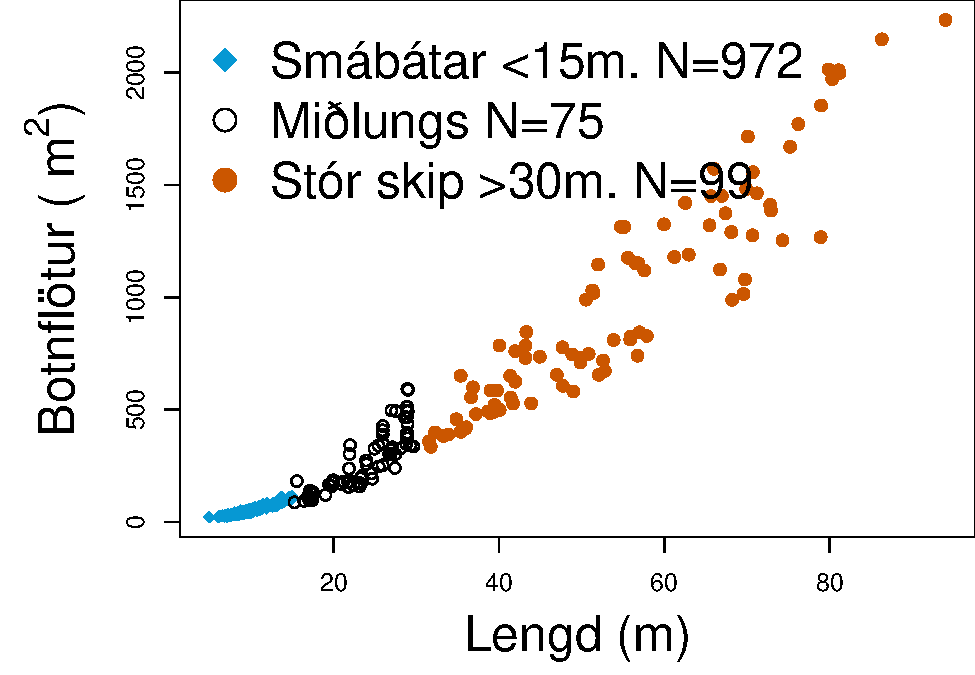
\includegraphics[width=0.5\linewidth]{OrplastHaf_files/figure-latex/slippur-1} 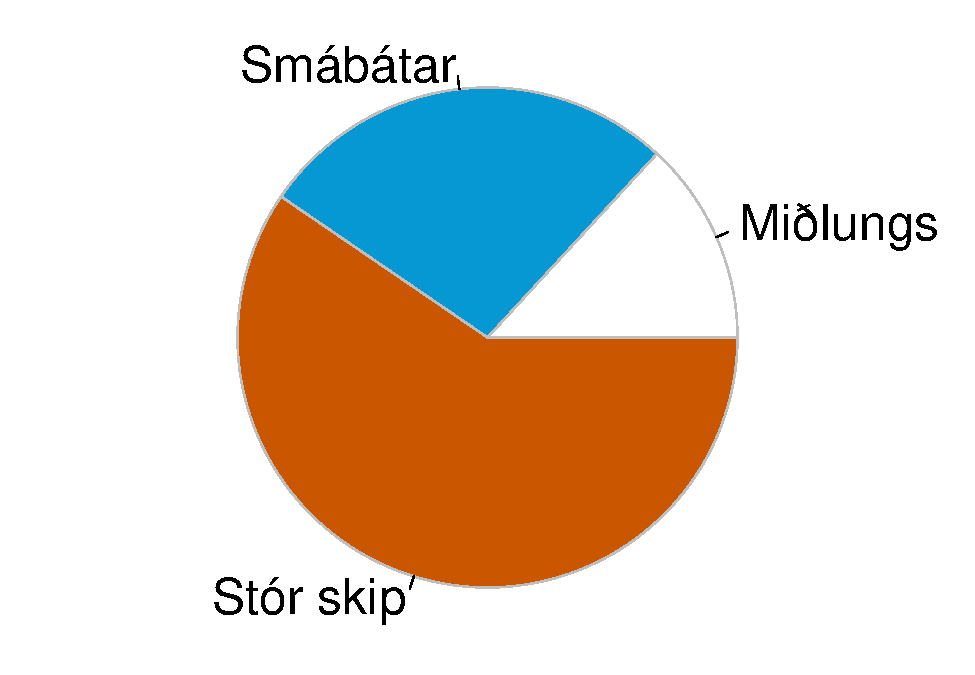
\includegraphics[width=0.5\linewidth]{OrplastHaf_files/figure-latex/slippur-2} 

}

\caption{Samband skipslengdar og botnflatar. Kökuritið sýnir hlutfall flatarmáls íslenskra fiskiskipa í þremur stærðarflokkum: Undir 15 metra löng skip, milli 15 og 30 metra löng og yfir 30 metra löng. Fengið með jöfnu frá Moser (2016)}\label{fig:slippur}
\end{figure}

Þar sem það eru engin neðri mörk á stærð báta sem geta farið í slipp eru mörkin óljós en hér er skipum skipt í 3 stærðarflokka: Undir 15 metra löng skip, milli 15 og 30 metra löng og yfir 30 metra löng. Litlir bátar, undir \textless{}10 metrar á lengd, eru sjaldnast settir í slipp og reiknum við því með að þeir séu að mestu leyti málaðir af eigendum uppi á landi og flyksurnar af háþrýstiþvotti á þeim fari í jarðveginn í mismikilli fjarlægð frá sjó. Stærri bátar og skip eru tekin í slipp niðri við sjó.

\hypertarget{smabatar}{%
\subsubsection*{Smábátar}\label{smabatar}}
\addcontentsline{toc}{subsubsection}{Smábátar}

Smábátar eru bátar undir 15 metrum að lengd. Smábátar nota um 2 til 2,5 L (eða 1-1,3 kg/L) af málningu á ári\textsuperscript{\protect\hyperlink{ref-Verschoor2016}{86}} eða 972-1236 kg/ári. Miðað við að hlutfall plastefna geti verið milli 30\% og 80\% og að upp undir 40\% falli til við háþrýstiþvott\textsuperscript{\protect\hyperlink{ref-Verschoor2016}{86}} er örplastlosun í umhverfið frá smábátum undir einu tonni á ári. Þar sem smábátar eru gjarnan málaðir af eigendum uppi á landi fer hluti þessarar losunar í jarðveginn og berst því ekki í hafið.

\hypertarget{strri-skip}{%
\subsubsection*{Stærri skip}\label{strri-skip}}
\addcontentsline{toc}{subsubsection}{Stærri skip}

Séu stór skip máluð á þriggja til fimm ára fresti er ekki ólíklegt að þau losi að því sem nemur einni stærðargráðu meira af örplasti í hafið. Þá er ekki tekið með það sem fýkur burtu við sprautumálun\textsuperscript{\protect\hyperlink{ref-OECD2009}{5}} sem getur verið umtalsvert þar sem hérlendir slippir eru ekki yfirbyggðir. Mesta mögulega losun örplasts frá slippunum er þó vegna háþrýstiþvottar

Í hollenskri rannsókn (Verschoor, 2016)\textsuperscript{\protect\hyperlink{ref-Verschoor2016}{86}} var áætlað að 14.830 tonn af málningu færu á 1.250 skip eða um 11,8 tonn á skip. Þar var um að ræða stór skip með 4-6 metra hæð undir vatnslínu. Miðað við að hlutfall plastefna geti verið milli 30\% og 80\% og að 10\% - 40\% falli til við háþrýstiþvott\textsuperscript{\protect\hyperlink{ref-Verschoor2016}{86}} er örplastlosunin mögulega 0,6-2,6 t af á skip. Ekki fengust tölur um fjölda og stærð skipa sem þjónustuð eru í slippum hérlendis árlega en sé tekið dæmi um stóru slippina fjóra, sem eru í Grindavík, Hafnafirði, Reykjavík og Akureyri, þá má ætla að hvert skip sé um tvær vikur í slipp. Þá eru hugsanlega um 100 stór skip á ári tekin í slipp hérlendis, íslensk og erlend. Það má því áætla að 60-260 tonn af örplasti falli til vegna stórra skipa í slipp og þá eru dráttarbrautirnar ekki meðtaldar.

Líftími (tíminn milli þess sem skipið er málað) skipamálningar er almennt styttri en hjá húsamálningu og því er sundrun vegna veðrunar kannski ekki eins há tala. Eflaust veldur veðrun sundrun plastefna í skipamálningu að hluta en ólíklegt er að nokkur sundrun eigi sér stað undir vatnsyfirborðinu. Ekki er vitað með hvaða hraða þær málningarflyksur sem liggja í jarðvegi eftir háþrýstiþvott í slipp sundrast en samkvæmt ónefndum heimildarmönnum hjá slippunum sjálfum er nánast allt sem fellur til vegna háþrýstiþvotta hreinsað upp úr flotkvíunum en hjá slippunum með dráttarbrautir er hreinsað upp eftir hentisemi.

Í fyrrnefndri hollenskri rannsókn\textsuperscript{\protect\hyperlink{ref-Verschoor2016}{86}} var reiknað með því að aðeins 3\% af því sem fellur til við háþrýstiþvott í slippum berist í hafið en þar í landi voru reglur hertar árið 1985 sem urðu til þess að farið var að hreinsa affallsvatn í slippum. Hérlendis er óheimilt að losa þrávirk efni í hafið og því er viðbúið að þessum úrgangi sé fargað eftir réttum leiðum. Því er áætlað að losun örplasts í hafið frá fjórum stærstu slippum hérlendis sé svipuð og áætluð hjá (Verschoor, 2016)\textsuperscript{\protect\hyperlink{ref-Verschoor2016}{86}} allt að 2 - 7,8 tonn.

Þar sem viðnám skipsbolsins við hafflötinn er mjög lítið er áætlað að aðeins um 1\% botnmálningar losni af vegna slits, aðallega við núning við bryggju\textsuperscript{\protect\hyperlink{ref-OECD2009}{5}}. Í tilfelli smábáta væri það mjög lág tala en fyrir þau 59 skip sem eru yfir 50 metrar á lengd og ætla má að yfir 10 tonn af málningu þurfi til að fullmála er 1\% slit um 6 t á 3 - 5 ára fresti. Því er áætlað að losun örplasts í hafið vegna skipamálningar geti verið á bilinu \textbf{3,2 - 10 t á ári}.

\hypertarget{frumplast-i-plastframleislu}{%
\section*{Frumplast í plastframleiðslu}\label{frumplast-i-plastframleislu}}
\addcontentsline{toc}{section}{Frumplast í plastframleiðslu}

Frumplast er ekki framleitt á Íslandi en er engu að síður flutt inn í þónokkru magni til framleiðslu á hinum ýmsu plasthlutum, t.d. fiskikörum, heitum pottum og trefjaplastbátum. Í þeim löndum þar sem frumplast er framleitt, t.d. Noregi og Svíþjóð, er gert ráð fyrir að losun í umhverfið sé í kringum 0,4\%\textsuperscript{\protect\hyperlink{ref-sundt2014sources}{32}} en aðrar forsendur eiga við í löndum þar sem frumplast er eingöngu innflutt\textsuperscript{\protect\hyperlink{ref-lassen2015microplastics}{78}}.

Fyrirtæki sem stunda plastframleiðslu í Danmörku notast eingöngu við innflutt frumplast líkt og hérlendis, aðallega frá Þýskalandi. Nokkur fyrirtæki í plastframleiðslu í Danmörku sem tóku þátt í átaki til að sporna við sóun á plastefni í framleiðsluferli sínu svöruðu því til að um 0,04\% af þeirra hráefni færi til spillis en aðeins litlum hluta þess væri sópað í niðurföll eða 0,0013\% hið mesta og engin losun væri beint í umhverfið\textsuperscript{\protect\hyperlink{ref-lassen2015microplastics}{78}}. Það má því áætla að hérlendis sé losun vegna frumplasts í plastframleiðslu frá 0,0005\% (sem er um helmingur af þeirri tölu). Engin gögn eru tiltæk um losun plasts í frumgerðum hérlendis en viðmið OECD er að í versta falli fari um 0,01\% efnisins til spillis við aðstæður þar sem lítil hætta er á sóun líkt og búast má við á Íslandi, helst er viðbúið að eitthvað efni glatist við flutning og meðhöndlun\textsuperscript{\protect\hyperlink{ref-OECD2009}{5}}.

Samkvæmt upplýsingum frá Tollstjóra fyrir árið 2017 og 2016 voru flutt inn um 12.600 tonn af plasti árlega í frumgerðum á borð við upplausnir, þeytur, deig eða önnur form (tollskrárnúmer 3901-3914). Það má því áætla að losun vegna frumplasts í plastframleiðslu sé frá 0,0005-0,01\% eða \textbf{0,06 - 1,3 tonn} árlega. Þó hefur ekki verið gerð könnun á því og matið er því annars vegar byggt á tölum sem framleiðendur í Danmörku gefa upp og hins vegar mati OECD frá iðnaði sem er mjög smár hér á landi. Þetta á bæði við um leka og sóun innandyra hjá framleiðslufyrirtækjunum og í flutningum og meðhöndlun.

\hypertarget{utisvi}{%
\section*{Útisvæði}\label{utisvi}}
\addcontentsline{toc}{section}{Útisvæði}

\hypertarget{gervigrasvellir}{%
\subsection*{Gervigrasvellir}\label{gervigrasvellir}}
\addcontentsline{toc}{subsection}{Gervigrasvellir}

Örplastmengun frá gervigrasvöllum er tvenns konar. Annars vegar vegna slits gervigrassins sjálfs og hins vegar vegna innfyllingar. Innfylling er það kallað þegar bætt er á gúmmíkurlið í gervigrasinu. Nokkrar gerðir gervigúmmís eru notaðar sem innfyllingarefni, algengast er að notað sé dekkjakurl en einnig er notast við annars konar dýrara efni. Kurlið er fínna en 5 mm og telst því til örplasts miðað við tilgang þessarar skýrslu. Viss hluti þess dreifist í kringum vellina með vindi, undir skóm og í fatnaði og einnig með snjómokstri eða skolast burtu með affallsvatni\textsuperscript{\protect\hyperlink{ref-Wredh2014}{110}}.

Allt að 140 tonn af gúmmíkurli geta verið í gervigrasinu á velli í fullri stærð\textsuperscript{\protect\hyperlink{ref-Wredh2014}{110}} en sé miðað við að um 30 mm lag af gúmmíkurli fínna en 5 mm vegi 426 kg/m\textsuperscript{3}\textsuperscript{\protect\hyperlink{ref-Gamalath2016}{111}} þá ættu að geta verið á milli 12 og 13 kg af gúmmíkurli á hverjum fermetra af gervigrasi. Misjafnt er eftir heimildum hve miklu innfyllingarefni er bætt á gervigrasvelli árlega en tölur frá 1 - 5\% liggja innan marka sem stuðst er við í þessari skýrslu\textsuperscript{\protect\hyperlink{ref-lassen2015microplastics}{78},\protect\hyperlink{ref-Hann2018}{103},\protect\hyperlink{ref-magnusson2016swedish}{112}}.

Samkvæmt Knattspyrnusambandi Íslands eru gervigrasvellir á Íslandi 197 talsins: 7 keppnishús, 26 keppnisvellir, 12 æfingavellir og smærri hús, 111 sparkvellir KSÍ og 43 aðrir sparkvellir. Alls eru þetta rúmlega 400.000 fermetrar, þar af um 13.000 m² með sandi sem innfyllingarefni en svart gúmmíkurl og annað iðnaðargúmmí er annars notað.

Til að meta losun innfyllingarefnis (gúmmíkurls) væri best að hafa nákvæm gögn um árlega áfyllingu á öllum völlum landsins en þau gögn eru ekki fyrirliggjandi og er því hér stuðst við áætlaðar tölur. Skv. Magnussen o.fl. 2014\textsuperscript{\protect\hyperlink{ref-magnusson2014mikroskrap}{113}} er mælt með því að á keppnisvöllum sé árlega bætt við 3-5 tonnum af fylliefni (420-700g/m2/ár miðað við 106x71 m völl). Á flestum völlum eru þó ekki gerðar sömu kröfur og á keppnisvöllum og má því búast við að losun sé oft á bilinu 2-3 tonn á ári (þ.e. 280-420g/m2/ár) eða jafnvel minni, einkum á minna notuðum völlum\textsuperscript{\protect\hyperlink{ref-magnusson2016swedish}{112}}.

Sumir vellir eru gerðir með gúmmímottu undir gervigrasinu sem minnkar þörfina á innfyllingu um allt að 50\% og þetta á við um helming íslenskra gervigrasvalla í fermetrum talið. Einnig er líklegt að kurlið þjappist niður í gervigrasið og því fer ekki allt innfyllingarefni til spillis út fyrir vellina.

Árlegri notkun dekkjakurls er skipt niður eftir gerðum leikvalla og miðast við að mest fari á keppnisvelli árlega en engu sé bætt á litla sparkvelli þar sem þeir voru flestir byggðir fyrir tiltölulega stuttu síðan og í millitíðinni skapaðist mikil umræða um mögulega skaðsemi innfyllingarefna og því beðið með að bæta á flesta þessa velli. Æfingavellir og smærri hús eru með losunartölur þarna mitt á milli.

Miðað við gögn frá Lassen\textsuperscript{\protect\hyperlink{ref-lassen2015microplastics}{78}} og FIFA tekin saman af\textsuperscript{\protect\hyperlink{ref-Hann2018}{103}} er gervigrasið sjálft u.þ.b. 0,8 - 1,4 kg/m2 og árlegt slit á bilinu 0.5 - 0.8\%. Sé miðað við 400.000 fermetra af gervigrasi á Íslandi er losun úr gervigrasinu sjálfu því undir hálfu tonni á ári.

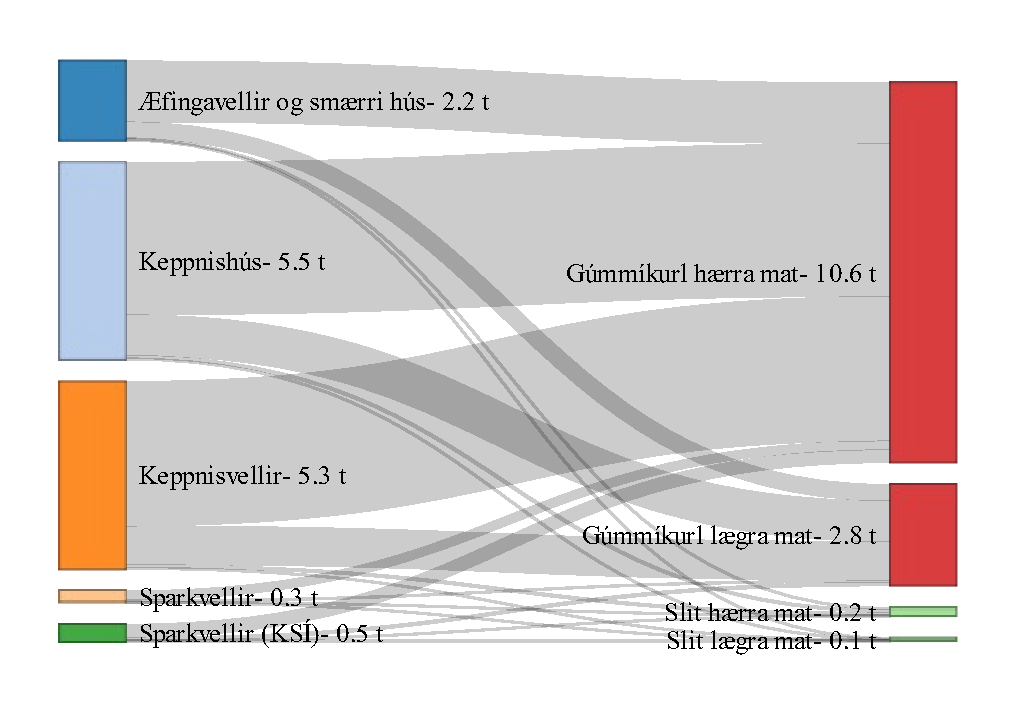
\includegraphics{OrplastHaf_files/figure-latex/unnamed-chunk-11-1.pdf}

Áætluð heildarlosun örplasts í umhverfið frá gervigrasvöllum á Íslandi árið 2017 er því 3-11 tonn, með þeim fyrirvara að matið byggir á almennum forsendum en ekki raunverulegum mælingum á áfyllingum gervigrasvalla á Íslandi. Erfitt er að meta hver afdrif þess eru og hve mikið fer í fráveitukerfi. Gúmmíkurlið festist í klæðnaði og undir skóm og getur borist í hafið í gegnum ræsi og frá affalli þvottavéla. Í breskri rannsókn\textsuperscript{\protect\hyperlink{ref-Hann2018}{103}} var áætlað að um 5\% innfyllingarefnis lendi í fráveitukerfum við vellina og önnur 5\% lendi í fráveitu frá búningsklefum og heimilum. Annars fari 90\% efnisins í förgun eða jarðveg. Miðað við þær forsendur má meta það sem svo að allt að 10\% geti borist með fráveitu í hafið eða \textbf{0,3 - 1,1 tonn}.

\hypertarget{skolaloir-og-leiksvi}{%
\subsection*{Skólalóðir og leiksvæði}\label{skolaloir-og-leiksvi}}
\addcontentsline{toc}{subsection}{Skólalóðir og leiksvæði}

Frá aldamótum hefur orðið mikil aukning á því að skólalóðir, leikskólalóðir og opin leiksvæði hafi fleti úr mjúkum gerviefnum á borð við gervigras, tartan (líkt og á frjálsíþróttahlaupabrautum), gúmmíhellur og gúmmígrasmottur. Þetta er gert til að skapa börnum öruggara umhverfi en allir þessir fletir innihalda gervigúmmí og verða þeir fyrir sliti vegna notkunar og veðrunar sem veldur losun örplasts í umhverfið. Ekki liggja fyrir gögn um örplastslosun þeirra á Íslandi en notkun og veðuraðstæður hafa mikil áhrif á umfang hennar.

Samkvæmt upplýsingum frá skipulagssviði Reykjavíkurborgar eru 39 grunnskólar, 75 leikskólar og 256 opin leiksvæði á þeirra vegum og umfang fyrrgreindra gerviefna á skólalóðum sé um 400-800 m², leikskólalóðum um 200-400 m² og opnum leiksvæðum 150-300 m². Flatarmál gerviefna í Reykjavík er þ.a.l. 69.000-138.000 m² og miðað við íbúafjölda Reykjavíkur 1. janúar 2017 (námundað að tugþúsundi, þ.e. 120.000) eru þetta 0,58-1,15 m² á hvern íbúa. Sé þetta hlutfall heimfært á íbúafjölda Íslands 1. janúar 2017 (námundað að tugþúsundi, þ.e. 340.000), eru gerviefni skólalóða og leikvalla á landinu 195.500-391.000 m² en þetta eru ónákvæmar tölur þar sem ekki liggur fyrir hvort hlutfallið í Reykjavík eigi við um önnur sveitarfélög á landinu. Til að áætla losun örplasts frá skólalóðum og leiksvæðum þarf einnig að vita hversu mikið slitið er, annaðhvort á ársgrundvelli eða líftíma mismunandi gerða gúmmíundirlags, en þau gögn eru ekki fyrirliggjandi. Ef gervigras á knattspyrnuvöllum eyðist um 0,5 - 0,8\% vegna notkunar má ætla að á leiksvæðum sé hlutfallið af svipaðri stærðargráðu en þó lægra en á íþróttavöllum. Miðað við 0,1 - 0,5\% má áætla að slit á gúmmíundirlagi á leikvöllum sé \textbf{0,2 - 2 tonn} árlega.

\hypertarget{neysluvara}{%
\section*{Neysluvara}\label{neysluvara}}
\addcontentsline{toc}{section}{Neysluvara}

\hypertarget{vottur-a-fatnai}{%
\subsection*{Þvottur á fatnaði}\label{vottur-a-fatnai}}
\addcontentsline{toc}{subsection}{Þvottur á fatnaði}

Gerviefni\footnote{Manngerð efni, annars vegar svokölluð syntetísk og hins vegar svokölluð gerviefni samkvæmt skilgreiningu í tollskrá: Tilbúnar trefjar í fatnaði: \textbf{Syntetísk (e. synthetic) efni}: Stutttrefjar og þræðir úr lífrænum fjölliðum sem framleiddar eru með fjölliðun lífrænna einliða til framleiðslu á fjölliðum, svo sem \textbf{pólýamíða, pólýestera, pólýólefína eða pólýúretana}, eða með kemískri umbreytingu á fjölliðum framleiddum með þessari aðferð (t.d. \textbf{póly(viníl alkóhól)} framleitt með vatnsrofi á \textbf{pólý (vínyl asetat)}).
  \textbf{Gerviefni (e. artificial)}: Með upplausn eða kemískri umbreytingu náttúrulegra lífrænna fjölliða (t.d. sellulósa) til framleiðslu á fjölliðum svo sem koparammoníumrayoni (kúpró) eða viskósarayoni eða með kemískri umbreytingu náttúrlegra lífrænna fjölliða (t.d. sellulósa, kaseíns og annarra prótína eða þörunga) til framleiðslu á fjölliðum svo sem sellulósaacetati eða algínötum.\textsuperscript{\protect\hyperlink{ref-tollur2017}{108}}} eru algeng í fatnaði og er þá um að ræða þræði úr plastefnum eins og t.d. pólýester en með þeim nást fram ýmsir eiginleikar á borð við fjölbreytta áferð, útlit og notagildi en þar ber helst að nefna slitþol, teygjanleika og vatnsheldni. Við þvott fatnaðar losnar þónokkuð magn þráða úr fatnaðinum og á það bæði við um fatnað úr gerviefnum (plastþráðum) og náttúrulegum efnum á borð við ull, silki og bómull\textsuperscript{\protect\hyperlink{ref-magnusson2014mikroskrap}{113},\protect\hyperlink{ref-magnusson2014mikroskopiska}{114}}.

Nælon (pólýamíð) var sett á markað í Bandaríkjunum árið 1939 og var fyrsta efnið unnið úr jarðefnaeldsneyti ætlað í vefnað\textsuperscript{\protect\hyperlink{ref-AmericanChemicalSociety1995}{115}}. Það greiddi leið fyrir önnur gerviefni sem fylgdu í kjölfarið eins og akríl 1949\textsuperscript{\protect\hyperlink{ref-masson1995acrylic}{116}} og pólýester 1951\textsuperscript{\protect\hyperlink{ref-brunnschweiler1993polyester}{117}} sem ruddu sér leið inn á heimsmarkaðinn á sjöunda áratugnum og voru loks framleidd í meira magni en bómull í lok tuttugustu aldarinnar\textsuperscript{\protect\hyperlink{ref-Shen2012}{118}}.

Plastþræðir gerviefna fara í skólp með niðurfalli þvottavéla til viðtakans, hvort sem það er rotþró\textsuperscript{\protect\hyperlink{ref-mahon2016microplastics}{119}} eða sjórinn. Seyra sem notuð er í landgræðslu getur þar af leiðandi verið uppspretta örplastmengunar í jarðvegi\textsuperscript{\protect\hyperlink{ref-mahon2016microplastics}{119}}. Mismunandi er hversu mikið af örplastþráðum hefur mælst í rennsli frá skólphreinsistöðvum\textsuperscript{\protect\hyperlink{ref-magnusson2014mikroskrap}{113},\protect\hyperlink{ref-napper2016release}{120}} eftir kröfum og tilkostnaði á hverju svæði. Á Íslandi er ekki gert ráð fyrir síun örplastagna í frárennsli en í (lögum um varnir gegn mengun hafs og stranda) {[}\url{https://www.althingi.is/lagas/149b/2004033.html?fbclid=IwAR0kTaxBydzlzPiAR28GAEQzKjRNQxBKqk4VEKCAhNn6AqYz58nsfSKrQJw}{]} segir að óheimilt sé að losa í hafið þrávirk gerviefni sem fljóta eða mara í hafinu en það er gert í miklum mæli í gegnum frárennsliskerfi hérlendis.

Til að áætla örplastmengun frá fataþvotti til sjávar á Íslandi er íbúafjöldi margfaldaður með áætluðum fjölda þvotta á ári og áætlaðri meðallosun örplastþráða við hvern þvott. Samkvæmt rannsókn sem gerð var á fataþvotti heimila víða um heim árið 2010\textsuperscript{\protect\hyperlink{ref-Pakula2010}{75}} eru þvegnir 165 þvottar að meðaltali á heimili á Íslandi. Áætlað er að hver þvottur í Vestur-Evrópu sé að meðaltali 3-4 kg og að hlutfall gerviefna í hverjum þvotti sé á bilinu frá 30-50\%\textsuperscript{\protect\hyperlink{ref-Pakula2010}{75}}. Fyrir hvert kíló af þvegnum fötum úr gerviefnum losna 12-640 mg af örplastþráðum\textsuperscript{\protect\hyperlink{ref-magnusson2016swedish}{112}}. Fjöldi heimila á Íslandi er um það bil 120 þúsund og samkvæmt neyslukönnun 2013-2016 er fjöldi í heimili 2,9.\footnote{Tölur fengnar af vef Hagstofunnar. (Mannfjöldi){[}\url{http://px.hagstofa.is/pxis/pxweb/is/Ibuar/Ibuar__mannfjoldi__2_byggdir__sveitarfelog/MAN02001.px/}{]}, (fjöldi heimila{[}\url{http://px.hagstofa.is/pxis/pxweb/is/Ibuar/Ibuar__manntal__1manntalfjolsk/CEN01050.px/}{]}), (fjöldi í heimili{[}\url{http://px.hagstofa.is/pxis/pxweb/is/Efnahagur/Efnahagur__visitolur__4a_neyslarannsokn/VIS05302.px/}{]})}

\begin{table}[t]

\caption{\label{tab:unnamed-chunk-12}Áætluð árleg losun örplasts frá þvotti í hafið á Íslandi.}
\centering
\begin{tabular}{lcc}
\toprule
  &  & Eining\\
\midrule
Fjöldi þvotta á ári & 165 & Þvottar\\
Fjöldi heimila & 120.000 & Heimili\\
Þyngd þvotta & 3-4 & kg\\
Þyngd örplasts fyrir hvert kg gerviefna & 12-640 & mg\\
Hlutfall gerviefna í þvotti & 30-50 & \% gerviefni\\
\bottomrule
\end{tabular}
\end{table}

Áætluð heildarlosun örplasts frá þvotti á Íslandi á ári er því \textbf{8,2-32 tonn}, með þeim fyrirvara að gögnin eru komin til ára sinna og gerviefni verða æ algengari í þvotti ásamt því að losun örplasts við hvern þvott er ekki föst stærð heldur breytileg eftir hversu notuð fötin eru.

\hypertarget{skosolar}{%
\subsection*{Skósólar}\label{skosolar}}
\addcontentsline{toc}{subsection}{Skósólar}

Skósólar eru gerðir úr gervigúmmíblöndu (nánar til tekið elastómerum sem eru ekki alltaf taldar til plasts), pólývínyl klóríð (e. PVC) eða pólýúretani\textsuperscript{\protect\hyperlink{ref-karak2009fundamentals}{121}} sem slitna við notkun skónna. Í danskri samantekt\textsuperscript{\protect\hyperlink{ref-lassen2015microplastics}{78}} var gerð tilraun til að meta örplastlosun frá skósólum í umhverfið út frá evrópsku mati á losun þalata\textsuperscript{\protect\hyperlink{ref-Pakalin2008}{122}} og umreiknað fyrir pólývínylklóríð (sem er plastefni). Þar er gróflega áætlað að slit skósóla sé á bilinu 100-1000 tonn árlega í Danmörku. Miðað við að íbúafjöldi Íslands sé um 6\% af íbúafjölda Danmerkur má áætla gróflega heildarlosun örplasts frá skósólum á Íslandi en ólík menning og veðurfar gerir beinan samanburð erfiðan.

\hypertarget{snyrtivorur}{%
\subsection*{Snyrtivörur}\label{snyrtivorur}}
\addcontentsline{toc}{subsection}{Snyrtivörur}

Örplast í snyrtivörum hefur verið talsvert í almennri umræðu á síðustu árum. Þekktustu áhrif sem fengin eru fram með örplastögnum í snyrtivörum eru skrúbbáhrif í sápum, andlitsskrúbbar og fótaskrúbbar. Þessar plastagnir hafa margskonar fleiri verkanir en engan möguleika á að vera endurunnar og berast að mestu beint í hafið eftir notkun. Það er þó svo að örplast í snyrtivörum telst aðeins vera smávægileg uppspretta á heildina litið.
Hlutfall örplasts getur verið allt á milli 1\%-90\% í ýmsum vörum og svo dæmi séu tekin eru það raksápur, ungbarnavörur, svitalyktareyðir, kinnalitir, hárlitunarefni og sjampó\textsuperscript{\protect\hyperlink{ref-Leslie2014}{123}}.

Í Evrópusambandsríkjunum er áætlað að um 800 tonnum af örplasti sé árlega bætt í snyrtivörur og þar af er um helmingur í handsápum sem eru ætlaðar til nota í iðnaði (t.d. á vélaverkstæðum)\textsuperscript{\protect\hyperlink{ref-Scudo2017}{124}}. Svipaðar tölur koma frá nokkrum skandinavískum samantektum eða undir 10 grömmum á ári á mann\textsuperscript{\protect\hyperlink{ref-sundt2014sources}{32},\protect\hyperlink{ref-lassen2015microplastics}{78},\protect\hyperlink{ref-magnusson2016swedish}{112}}.

Áætluð heildarlosun örplasts í hafið frá snyrtivörum á Íslandi er því \textbf{0,34-3,4 tonn}.

\hypertarget{haglaskot}{%
\subsection*{Haglaskot}\label{haglaskot}}
\addcontentsline{toc}{subsection}{Haglaskot}

Haglaskot í dag hafa yfirleitt tvo hluta með eða úr plasti: Skothylkið/patrónuna, sem er að hluta úr plasti, og forhlaðið sem er eingöngu úr plasti. Forhlaðið er staðsett milli púðurs og hagla inni í skothylkinu en einnig eru til skot sem innihalda ekkert plast, líkt og var eingöngu tilfellið fyrir fjöldaframleiðslu plasts, en notkun þeirra á Íslandi er lítil.

Í hvert skipti sem hleypt er af skoti fylgir forhlaðið (\textasciitilde{}2,0 grömm) höglunum út um hlaup byssunnar og týnist það yfirleitt út í umhverfið, nema á skotsvæðum þar sem stór hluti er hreinsaður upp reglulega. Utan skotsvæða er eitthvað um að forhlöð séu tínd upp en gera má ráð fyrir að það hlutfall sé lítið. Skothylkin sitja hins vegar eftir í hlaupinu (í tvíhleypum) eða falla til hliðar (úr hálfsjálfvirkum haglabyssum) og er því auðvelt að tína upp líkt og ábyrgir skotveiðimenn stunda af metnaði. Eitthvað er um að þau séu skilin eftir á víðavangi en að því sögðu er einnig algengt að skotveiðimenn týni upp skothylki eftir aðra.

Að áætla magn forhlaða sem fara í umhverfið er því nokkuð einfalt ef fjöldi skota er þekktur. Erfiðara er hins vegar að áætla magn skothylkja sem enda í umhverfinu og er með fyrirliggjandi gögnum ekki hægt að álykta nánar en að líklega sé um minnihluta sé að ræða.

Samkvæmt óformlegum heimildum innan skotveiðigeirans má áætla að fjöldi notaðra haglaskota, bæði fyrir veiði og leirdúfur, hafi árið 2017 verið u.þ.b. 1.600.000 og hafi árið 2018 verið upp undir 2.000.000. Þessi aukning sé rakin til aukinna vinsælda og sölu leirdúfuskota en skiptingin í ár sé líklega \textasciitilde{}1.400.000 leirdúfuskot (yfirleitt 35 grömm) og \textasciitilde{}600.000 veiðiskot (yfirleitt 55 grömm). Af því má álykta að árið 2017 hafi leirdúfuskot gróflega verið \textasciitilde{}1.000.000 og veiðiskot \textasciitilde{}600.000, með fyrirvara um óþekkt skekkjumörk. Séu þessar tölur bornar saman við gögn frá Tollstjóra voru árið 2017 flutt inn 36,8 tonn af skothylkjum fyrir haglabyssur (tollskrárnúmer 9306.2100) og sé miðað við algengar þyngdir haglaskota ( 35-55 grömm) fást tölur af sömu stærðargráðu. Því má ætla að þessar tölur séu lýsandi, með áðurgreindum fyrirvara um ótilgreind skekkjumörk.

Heildarmagn notaðra forhlaða árið 2017 var því 3,2 tonn en þar sem ákveðið hlutfall er notað á skotsvæðum, hvar hægt er að hreinsa forhlöðin upp, er ljóst að einungis hluti forhlaða endar í umhverfinu þrátt fyrir að nánast öll forhlöð í skotveiði glatist í umhverfið. Hlutfall þeirra forhlaða sem týnast í umhverfið er því erfitt að meta án frekari rannsókna en þrátt fyrir það ríkir nokkur vissa um stærðargráðuna.

Áætluð heildarlosun örplasts frá haglaskotum á Íslandi árið 2017 er því \textbf{1-3 tonn}, með fyrirvara um ofangreinda óvissuþætti. Ekki er unnt að áætla afdrif örplasts frá haglaskotum að svo stöddu.

\hypertarget{matvlaframleisla}{%
\section*{Matvælaframleiðsla}\label{matvlaframleisla}}
\addcontentsline{toc}{section}{Matvælaframleiðsla}

\hypertarget{sjavarutvegur}{%
\subsection*{Sjávarútvegur}\label{sjavarutvegur}}
\addcontentsline{toc}{subsection}{Sjávarútvegur}

Veiðarfæri eru almennt úr plastefnum, hvort sem það eru línur, net, flotholt og eru því möguleg uppspretta örplastmengunar, annars vegar vegna slits við venjulega notkun og hins vegar vegna veiðarfæra sem tapast í hafið og veðrast. Í umhverfisskýrslu Samtaka fyrirtækja í sjávarútvegi er tekið fram að um 1.300 tonnum af veiðarfærum sé skilað til hafna og þaðan til endurvinnslu (eða viðeigandi förgunar). Ekki eru til upplýsingar um heildarmagn veiðarfæra í notkun á Íslandsmiðum. Magn veiðarfæra íslenska fiskveiðiflotans var gróflega áætlað um 7.313 tonn út frá heildarþyngd afla borið saman við önnur evrópuríki\textsuperscript{\protect\hyperlink{ref-Hann2018}{103}}. Samkvæmt sérfræðingi Hafrannsóknarstofnunar er sú tala allt of há þar sem fæstar fiskveiðiþjóðir eru með eins fáa báta miðað við hvert veitt kíló af fiski og því betri nýtingu á veiðarfærum.

Losun örplasts fer eftir því hvernig veiðarfæri um ræðir en sum þeirra slitna og missa þræði við notkun í mismiklum mæli. Aðrar gerðir veiðarfæra líkt og grásleppunet og handfæralínur slitna ekki með þeim hætti. Í sænskri rannsókn var losun örplasts metin 1-10\% af heildarþyngd veiðarfæra sænskra fiskiskipa\textsuperscript{\protect\hyperlink{ref-Hann2018}{103}} með þeim fyrirvara að bæði tölurnar um heildarþyngd veiðarfæra og losun örplasts væru byggðar á veikum grunni. Það er nauðsynlegt að afla upplýsinga um magn veiðarfæra á íslenskum miðum áður en hægt er að leggja nákvæmt mat á hversu hátt hlutfall veiðarfæra fellur til við notkun á ársgrundvelli. Varðandi almenna veðrun veiðarfæra og slit er einnig þörf á frekari upplýsingum eða rannsóknum\textsuperscript{\protect\hyperlink{ref-Hann2018}{103}}.

\hypertarget{sjokviaeldi}{%
\subsection*{Sjókvíaeldi}\label{sjokviaeldi}}
\addcontentsline{toc}{subsection}{Sjókvíaeldi}

Mannvirki og búnaður í sjókvíaeldi er að töluverðu leyti úr plasti, til dæmis net, rör, flotholt ofl. og er viðbúið að eitthvað af örplasti losni vegna slits og veðrunar. Öll slík losun fer óhjákvæmilega beint í hafið en ekki hefur tekist að nálgast mælingar eða gögn um þessa losun eða stærðargráðu hennar. Norsk skýrsla um losun örplasts\textsuperscript{\protect\hyperlink{ref-sundt2014sources}{32}} fjallaði stuttlega um örplastmengun frá sjókvíaeldi en vísaði ekki í töluleg gögn. Því er þörf á frekari gögnum, t.d. í formi staðlaðrar losunar af örplastögnum fyrir hverja gerð sjókvíar, enda viðbúið að einhver munur sé á milli hönnunar ólíkra framleiðenda.
Samkvæmt Matvælastofnun eru samtals um 73 sjókvíar í notkun á Íslandi 2018 á Vestfjörðum og Austfjörðum og flokkast þær allar sem stórar kvíar eða 160 metrar í ummál. Með stöðluðum losunartölum fyrir sjókvíar að þessu tagi væri því hægt að áætla heildarlosun á landsvísu.

Ekki er að svo stöddu hægt að áætla heildarlosun örplasts frá sjókvíaeldi á Íslandi vegna skorts á gögnum og auk þess ríkir óvissa um stærðargráðu losunarinnar, einkum í ljósi mikils vaxtar atvinnugreinarinnar.

\hypertarget{landbunaur-heyrulluplast}{%
\subsection*{Landbúnaður (heyrúlluplast)}\label{landbunaur-heyrulluplast}}
\addcontentsline{toc}{subsection}{Landbúnaður (heyrúlluplast)}

Heyrúlluplast getur lent í umhverfinu og orðið að örplasti en erfitt er að áætla að hversu miklu leyti. Notkun er t.d. breytileg eftir árferði og innflutningstölur fyrir tiltekið ár því ekki endilega lýsandi, auk þess sem notuðu plasti getur verið skilað til móttökuaðila á öðru ári en það var notað. Til að taka mið af þessu er því hér byggt á meðaltali fyrir árin 2013-2017, bæði varðandi innflutning og magn sem skilað hefur verið til móttökuaðila. Samkvæmt Úrvinnslusjóði þarf hér að gera ráð fyrir því að heyrúlluplast geti við notkun þyngst um allt að 30\%, vegna raka og drullu, en almennt er gert ráð fyrir um 20-25\% þyngdaraukningu (Úrvinnslusjóður, munnleg heimild).
Innflutningur heyrúlluplasts á árunum 2013-2018 var að meðaltali tæplega 2.000 tonn\textsuperscript{\protect\hyperlink{ref-Urvinnslusjouxf0ur2016}{125},\protect\hyperlink{ref-tollurinn}{126}} og má því ætla að árleg notkun sé af þeirri stærðargráðu. Á árunum 2013-2016 var að meðaltali skilað inn 2.094 tonnum af notuðu heyrúlluplasti\textsuperscript{\protect\hyperlink{ref-Urvinnslusjouxf0ur2016}{125}}, sem annaðhvort fór í endurvinnslu, var urðað eða fargað, og sé gert ráð fyrir 20-25\% þyngdaraukningu vegna raka og drullu má ætla að það hafi upprunalega verið í kringum 1.700 tonn. Sé tekið mið af þessum forsendum má gera ráð fyrir að árlega endi um 300 tonn af heyrúlluplasti annaðhvort í almennri urðun eða umhverfinu. En ekki hefur verið metið hversu mikið fer í almenna urðun annars vegar og umhverfið hins vegar.

\hypertarget{umhverfi}{%
\section*{Umhverfi}\label{umhverfi}}
\addcontentsline{toc}{section}{Umhverfi}

\hypertarget{plast-i-fjorum}{%
\subsection*{Plast í fjörum}\label{plast-i-fjorum}}
\addcontentsline{toc}{subsection}{Plast í fjörum}

Niðurbrot plastrusls gerist hve hraðast í orkumiklum kerfum líkt og fjörum en plastrusl í hafi og í fjörum er álitið vera með stærstu uppsprettum örplasts í hafinu\textsuperscript{\protect\hyperlink{ref-andrady2011microplastics}{37}}. Ekki er hægt að meta magn af örplasti sem berst frá niðurbroti plastsrusls í fjörum í hafið. Magn rusls er ekki gott að áætla og svo vantar gögn um það hve hratt plasthlutir mást og eyðast í fjörum og sundrast frá stærra plasti í örplastsagnir.

Skipulagðar hreinsanir á Íslandi eru framkvæmdar af félagasamtökunum Bláa hernum. Samkvæmt talsmanni þeirra er um eitt tonn af plastrusli á hverjum kílómetra af strandlengju sem þau hreinsa. Veiðarfæri og umbúðir úr plasti eru yfir 95\% af þyngd hlutanna sem finnast. Veiðarfærin geta verið stórar einingar upp á hundruð kílóa en umbúðirnar eru oft smærri ílát fyrir neysluvöru.

\begin{figure}
\centering
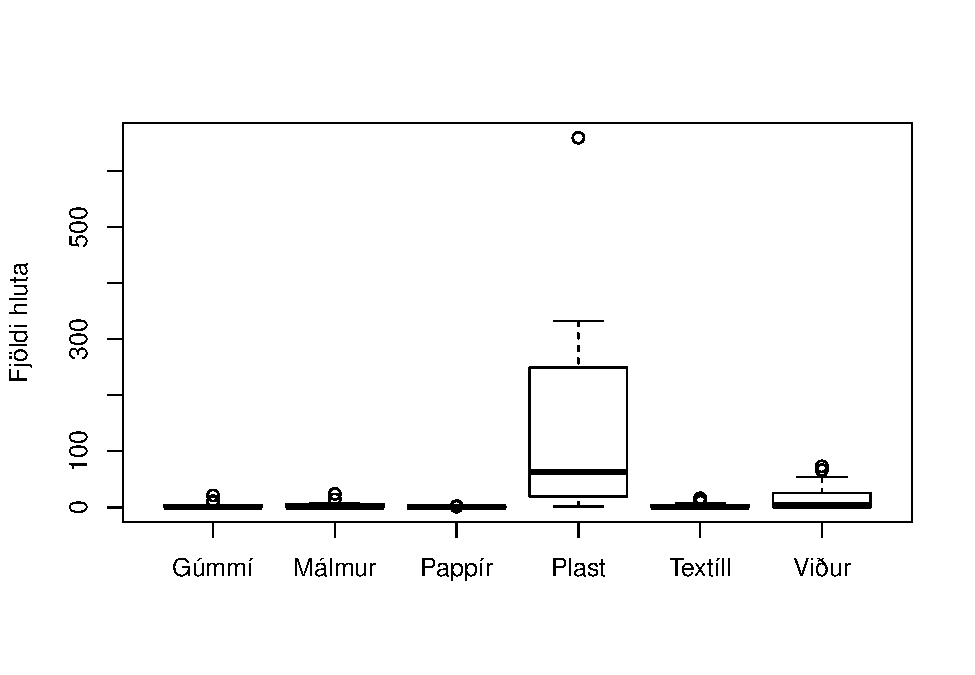
\includegraphics{OrplastHaf_files/figure-latex/ospartafla-1.pdf}
\caption{\label{fig:ospartafla}Rusl í fjörum á Íslandi. Unnið eftir gögnum frá OSPAR.}
\end{figure}

Vaktanir á íslenskum fjörum eru gerðar eftir OSPAR samkomulaginu en þar eru 100 metra fjörukaflar teknir fyrir og skrásettur fjöldi hluta og hvers eðlis þeir eru en þeir eru ekki vigtaðir. Ábyggilegt er að við staðarval sé tekið mið af sjáanlegri mengun, sérstaklega hjá Bláa hernum en einnig hjá OSPAR og því eru gögnin þeirra skekkt í átt að meiri mengun en almennt finnst í íslenskum fjörum. Skráðar hafa verið 18 hreinsanir á fimm 100 metra strandlengjupörtum á Íslandi í \href{http://www.mcsuk.org/ospar/map}{OSPAR gagnagrunninn}\textsuperscript{\protect\hyperlink{ref-ospar2019}{127}}. Niðurstöður þeirra sýna að plast er meirihluti þeirra hluta sem finnast í fjörum eða um 83\% (sjá mynd \ref{fig:ospartafla}).

\hypertarget{sigvatn-fra-sorpurunarstovum}{%
\subsection*{Sigvatn frá sorpurðunarstöðvum}\label{sigvatn-fra-sorpurunarstovum}}
\addcontentsline{toc}{subsection}{Sigvatn frá sorpurðunarstöðvum}

Urðaður heimilisúrgangur er um 60.000 tonn á ári\textsuperscript{\protect\hyperlink{ref-tollurinn2}{128}} á ýmsum urðunarstöðvum á Íslandi. Tugir urðunarstöðva eru vítt og breitt um landið, sumar þeirra eru þó ekki lengur í notkun. Stærsta urðunarstöðin á Álfsnesi í Reykjavík er með leyfi til að taka við 120.000 tonnum á ári en aðrar stórar stöðvar eru í Glerárdal í Eyjafirði og í Stekkjavík við Húnaflóa (báðar um 20.000 tonn) og við Ölfusá er stöð með leyfi fyrir 30.000 tonnum. Aðrar minni stöðvar hafa leyfi fyrir nokkrum hundruðum eða nokkur þúsundum tonna.

Rannsóknir á örplastinnihaldi í sigvatni benda ekki til þess að það sé mikilvæg uppspretta örplasts\textsuperscript{\protect\hyperlink{ref-Praagh1277395}{129}}. Talningar á örplastsögnum úr sigvatni nokkurra urðunarstöðva á Íslandi voru til dæmis lægri en talningar úr skólpi\textsuperscript{\protect\hyperlink{ref-Praagh1277395}{129}}. Í stærstu urðunarstöðinni á Álfsnesi mældist örplast í mestu magni (frá 50-5000 μm að stærð) og var árleg losun metin á bilinu \textbf{0,002 - 177 kg}\textsuperscript{\protect\hyperlink{ref-Praagh1277395}{129}}.

\hypertarget{samantekt-og-lokaor}{%
\section*{Samantekt og lokaorð}\label{samantekt-og-lokaor}}
\addcontentsline{toc}{section}{Samantekt og lokaorð}

\begin{Shaded}
\begin{Highlighting}[]
\NormalTok{nafn <-}\StringTok{ }\KeywordTok{c}\NormalTok{(}\StringTok{"Bifreiðahjólbarðar"}\NormalTok{, }\StringTok{"Vegmerkingar"}\NormalTok{, }\StringTok{"Flugvélahjólbarðar"}\NormalTok{, }\StringTok{"Húsamálning"}\NormalTok{, }\StringTok{"Skipamálning"}\NormalTok{, }\StringTok{"Gervigras"}\NormalTok{, }\StringTok{"Leikvellir"}\NormalTok{, }\StringTok{"Þvottur"}\NormalTok{, }\StringTok{"Snyrtivörur"}\NormalTok{, }\StringTok{"Haglaskot"}\NormalTok{, }
  \StringTok{"Sigvatn"}\NormalTok{)}

\NormalTok{lagt <-}\StringTok{ }\KeywordTok{c}\NormalTok{(}\DecValTok{371}\NormalTok{, }\DecValTok{41}\NormalTok{, }\DecValTok{26}\NormalTok{, }\FloatTok{33.2}\NormalTok{, }\DecValTok{60}\NormalTok{, }\DecValTok{3}\NormalTok{, }\FloatTok{0.2}\NormalTok{, }\FloatTok{8.2}\NormalTok{, }\FloatTok{0.34}\NormalTok{, }\DecValTok{1}\NormalTok{, }\FloatTok{0.002}\NormalTok{)}
\NormalTok{hatt <-}\StringTok{ }\KeywordTok{c}\NormalTok{(}\DecValTok{586}\NormalTok{, }\DecValTok{256}\NormalTok{, }\DecValTok{50}\NormalTok{, }\FloatTok{77.1}\NormalTok{, }\DecValTok{260}\NormalTok{, }\DecValTok{11}\NormalTok{, }\DecValTok{2}\NormalTok{, }\DecValTok{32}\NormalTok{, }\FloatTok{3.4}\NormalTok{, }\DecValTok{3}\NormalTok{, }\FloatTok{0.177}\NormalTok{)}
\NormalTok{losun <-}\StringTok{ }\KeywordTok{c}\NormalTok{(}\DecValTok{164}\NormalTok{, }\FloatTok{5.7}\NormalTok{, }\OtherTok{NA}\NormalTok{, }\FloatTok{15.2}\NormalTok{, }\FloatTok{3.2}\NormalTok{, }\FloatTok{0.3}\NormalTok{, }\OtherTok{NA}\NormalTok{, }\FloatTok{8.2}\NormalTok{, }\FloatTok{0.34}\NormalTok{, }\OtherTok{NA}\NormalTok{, }\FloatTok{0.002}\NormalTok{)}
\NormalTok{losunb <-}\StringTok{ }\KeywordTok{c}\NormalTok{(}\DecValTok{234}\NormalTok{, }\FloatTok{42.6}\NormalTok{, }\OtherTok{NA}\NormalTok{, }\FloatTok{36.1}\NormalTok{, }\DecValTok{10}\NormalTok{, }\FloatTok{1.1}\NormalTok{, }\OtherTok{NA}\NormalTok{, }\DecValTok{32}\NormalTok{, }\FloatTok{3.4}\NormalTok{, }\OtherTok{NA}\NormalTok{, }\FloatTok{0.177}\NormalTok{)}

\NormalTok{tafla <-}\StringTok{ }\KeywordTok{data.frame}\NormalTok{(nafn, lagt, hatt, losun, losunb)}
\KeywordTok{names}\NormalTok{(tafla) <-}\StringTok{ }\KeywordTok{c}\NormalTok{(}\StringTok{""}\NormalTok{, }\StringTok{"Hærra mat"}\NormalTok{, }\StringTok{"Lægra mat"}\NormalTok{, }\StringTok{"Hærra mat"}\NormalTok{, }\StringTok{"Lægra mat"}\NormalTok{)}
\NormalTok{tafla <-}\StringTok{ }\KeywordTok{format}\NormalTok{(tafla, }\DataTypeTok{decimal.mark =} \StringTok{","}\NormalTok{, }\DataTypeTok{big.mark =} \StringTok{"."}\NormalTok{, }\DataTypeTok{drop0trailing =}\NormalTok{ T)}
\KeywordTok{require}\NormalTok{(kableExtra)}

\ControlFlowTok{if}\NormalTok{ (knitr}\OperatorTok{::}\KeywordTok{is_html_output}\NormalTok{()) \{}
\NormalTok{  knitr}\OperatorTok{::}\KeywordTok{kable}\NormalTok{(tafla, }\DataTypeTok{booktabs =}\NormalTok{ T, }\DataTypeTok{align =} \StringTok{"c"}\NormalTok{, }\DataTypeTok{caption =} \StringTok{"Samantekt á þeim uppsprettum örplasts sem kannaðar voru og mat á losun frám þeim í hafið"}\NormalTok{) }\OperatorTok\StringTok{ }
\StringTok{    }\KeywordTok{kable_styling}\NormalTok{(}\StringTok{"striped"}\NormalTok{, }\DataTypeTok{full_width =}\NormalTok{ T) }\OperatorTok\StringTok{ }\KeywordTok{add_header_above}\NormalTok{(}\KeywordTok{c}\NormalTok{(}\StringTok{`}\DataTypeTok{ }\StringTok{`}\NormalTok{ =}\StringTok{ }\DecValTok{1}\NormalTok{, }\StringTok{`}\DataTypeTok{Uppspretta (t)}\StringTok{`}\NormalTok{ =}\StringTok{ }\DecValTok{2}\NormalTok{, }\StringTok{`}\DataTypeTok{Losun í haf (t)}\StringTok{`}\NormalTok{ =}\StringTok{ }\DecValTok{2}\NormalTok{)) }\OperatorTok\StringTok{ }\KeywordTok{column_spec}\NormalTok{(}\DecValTok{1}\NormalTok{, }\DataTypeTok{bold =}\NormalTok{ T)}
\NormalTok{\} }\ControlFlowTok{else}\NormalTok{ \{}
\NormalTok{  knitr}\OperatorTok{::}\KeywordTok{kable}\NormalTok{(tafla, }\DataTypeTok{booktabs =}\NormalTok{ T, }\DataTypeTok{align =} \StringTok{"c"}\NormalTok{, }\DataTypeTok{caption =} \StringTok{"Samantekt á þeim uppsprettum örplasts sem kannaðar voru og mat á losun frám þeim í hafið"}\NormalTok{)}
  
\NormalTok{\}}
\end{Highlighting}
\end{Shaded}

\label{tab:unnamed-chunk-13}Samantekt á þeim uppsprettum örplasts sem kannaðar voru og mat á losun frám þeim í hafið

Hærra mat

Lægra mat

Hærra mat

Lægra mat

Bifreiðahjólbarðar

371

586

164

234

Vegmerkingar

41

256

5,7

42,6

Flugvélahjólbarðar

26

50

NA

NA

Húsamálning

33,2

77,1

15,2

36,1

Skipamálning

60

260

3,2

10

Gervigras

3

11

0,3

1,1

Leikvellir

0,2

2

NA

NA

Þvottur

8,2

32

8,2

32

Snyrtivörur

0,34

3,4

0,34

3,4

Haglaskot

1

3

NA

NA

Sigvatn

0,002

0,177

0,002

0,177

Tölur um örplastlosun frá þvotti á fatnaði eru frá því 2010\textsuperscript{\protect\hyperlink{ref-pakula2010electricity}{130}} og eru þær því líklega vanmetnar þar sem fatnaður úr náttúrulegum efnum er á undanhaldi. Mikið af gerviefnum er á heimilum fólks, alls konar teppi og mottur, áklæði utan um sófa og stóla, tuskudýr og fleira í umhverfinu innadyra sem ekki er minnst á í þessari skýrslu getur talist til uppsprettu örplasts í hafið en ryk af heimilum fer mest í sorphirðu eða niðurföll.

Erlendar rannsóknir sem tengjast örplastlosun frá samgöngum og iðnaði er hægt að yfirfæra á Ísland þar sem þær eru byggðar á sterkari grunni þó svo vikmörkin séu stór, sérstaklega hvað varðar farleiðir til sjávar. Óvissa er hve mest um farleiðir örplasts frá dekkjaögnum, vegmerkingum, húsamálningu og fleiri þátta sem berast aðallega til sjávar með ofanvatni og um fráveitukerfi en ekki beina leið gegnum niðurföll. Með sýnatökum úr vegaskurðum og settjörnum tengdum frárennsli vega og jarðvegi í kringum vegi, flugvelli og aðrar uppsprettur í þéttbýli verður hægt að minnka þá óvissu.

Gera þarf könnun á innflutningi málningar og efna til framleiðslu á málningu þar sem mikil óvissa ríkir um hlutfallslegt magn ólíkrar málningar, til dæmis skipa- og húsamálningar og málningar með misháu fjölliðuinnihaldi hérlendis. Skýrsluhöfundum er ekki kunnugt um hvernig eftirliti með slippum er háttað en við matið á örplastlosun frá þeim var stuðst við tölur frá Hollandi\textsuperscript{\protect\hyperlink{ref-Verschoor2016}{86}} en engar samantektir á þeirra starfsemi fengust afhendar. Mesti munur á mögulegri uppsprettu og losun í hafið var frá slippunum fjórum en að sögn starfsmanna mismunandi slippa er nánast allt hreinsað upp sem fellur til vegna viðhalds skipa.

Í flokkunum tengdum matvælaframleiðslu og umhverfi var hve minnstar upplýsingar að finna um uppsprettur örplasts. Þó svo að rannsóknir á magni og niðurbroti plasts í sjávarumhverfinu hafi verið rannsakaðar að einhverju leyti\textsuperscript{\protect\hyperlink{ref-Andrady2017}{2}} þá eru upplýsingar enn af of skornum skammti til að meta örplastlosun í fjörum hérlendis. Það er þó eflaust tilfinnanlegt magn. Svipaða sögu er að segja af heyrúlluplasti og veiðarfærum en magn þess sem er flutt inn og fært til endurvinnslu er ágætlega þekkt en afdrif þess sem lendir í umhverfinu eru ókunn enn.

Við gerð þessarar skýrslu var aðallega notast við

\hypertarget{heimildir}{%
\chapter*{Heimildir}\label{heimildir}}
\addcontentsline{toc}{chapter}{Heimildir}

\hypertarget{refs}{}
\leavevmode\hypertarget{ref-geyer2017production}{}%
1. Geyer R, Jambeck JR, Law KL. Production, use, and fate of all plastics ever made. \emph{Science advances}. 2017;3(7):e1700782.

\leavevmode\hypertarget{ref-Andrady2017}{}%
2. Andrady AL. The plastic in microplastics: A review. \emph{Marine Pollution Bulletin}. 2017;119(1):12--22. doi:\href{https://doi.org/10.1016/j.marpolbul.2017.01.082}{10.1016/j.marpolbul.2017.01.082}

\leavevmode\hypertarget{ref-Gowariker2005}{}%
3. Gowariker N og S V.R. og Viswanathan. \emph{Polymer science}. New Age International (P) Limited Publishers, New Delhi, India; 2005.

\leavevmode\hypertarget{ref-Gudjonsdottir2015}{}%
4. Guðjónsdóttir K. Snertiefni matvæla. Í: Fræðslufundur Matvælastofnunar; 2015:56. \url{http://www.mast.is/library/Fyrirlestrar/snertiefnimatvaela150414KG.pdf}.

\leavevmode\hypertarget{ref-OECD2009}{}%
5. OECD. Emission Scenario Document on Plastics Additives. Í: \emph{OECD Series on Emission Scenario Documents}.; 2009:141. \url{http://tinyurl.com/y352gwu9}.

\leavevmode\hypertarget{ref-karamanlioglu2017abiotic}{}%
6. Karamanlioglu M, Preziosi R, Robson GD. Abiotic and biotic environmental degradation of the bioplastic polymer poly (lactic acid): a review. \emph{Polymer Degradation and Stability}. 2017;137:122--130.

\leavevmode\hypertarget{ref-tsuji2002environmental-1}{}%
7. Tsuji H, Suzuyoshi K. Environmental degradation of biodegradable polyesters 1. Poly (\(\varepsilon\)-caprolactone), poly {[}(R)-3-hydroxybutyrate{]}, and poly (L-lactide) films in controlled static seawater. \emph{Polymer Degradation and Stability}. 2002;75(2):347--355.

\leavevmode\hypertarget{ref-tsuji2002environmental-2}{}%
8. Tsuji H, Suzuyoshi K. Environmental degradation of biodegradable polyesters 2. Poly (\(\varepsilon\)-caprolactone), poly {[}(R)-3-hydroxybutyrate{]}, and poly (L-lactide) films in natural dynamic seawater. \emph{Polymer degradation and stability}. 2002;75(2):357--365.

\leavevmode\hypertarget{ref-hopewell2009plastics}{}%
9. Hopewell J, Dvorak R, Kosior E. Plastics recycling: challenges and opportunities. \emph{Philosophical Transactions of the Royal Society of London B: Biological Sciences}. 2009;364(1526):2115--2126.

\leavevmode\hypertarget{ref-Waters1972}{}%
10. Carpenter EJ, Anderson JS, Harvey RG, Miklas HP, Peck BB. Polystyrene Spherules in Coastal Waters. 1972;(NOVEMBER):0--2.

\leavevmode\hypertarget{ref-Colton1974}{}%
11. Colton JB, Knapp FD, Burns BR. Plastic Particles in Surface Waters of the Northwestern Atlantic. 1974;(August 1972):491--497.

\leavevmode\hypertarget{ref-zitko1991another}{}%
12. Zitko V, Hanlon M. Another source of pollution by plastics: skin cleaners with plastic scrubbers. \emph{Marine Pollution Bulletin}. 1991;22(1):41--42.

\leavevmode\hypertarget{ref-Thompson2004lost}{}%
13. Thompson RC, Olse Y. Lost at sea: where is all the plastic? \emph{Science (New York, NY)}. 2004;304(5672):838. doi:\href{https://doi.org/doi:10.1126/science.1094559}{doi:10.1126/science.1094559}

\leavevmode\hypertarget{ref-de2018impacts}{}%
14. Souza Machado AA de, Lau CW, Till J, o.fl. Impacts of microplastics on the soil biophysical environment. \emph{Environmental science \& technology}. 2018;52(17):9656--9665.

\leavevmode\hypertarget{ref-besseling2017fate}{}%
15. Besseling E, Quik JT, Sun M, Koelmans AA. Fate of nano-and microplastic in freshwater systems: A modeling study. \emph{Environmental Pollution}. 2017;220:540--548.

\leavevmode\hypertarget{ref-horton2017microplastics}{}%
16. Horton AA, Walton A, Spurgeon DJ, Lahive E, Svendsen C. Microplastics in freshwater and terrestrial environments: evaluating the current understanding to identify the knowledge gaps and future research priorities. \emph{Science of the total environment}. 2017;586:127--141.

\leavevmode\hypertarget{ref-eriksen2014plastic}{}%
17. Eriksen M, Lebreton LC, Carson HS, o.fl. Plastic pollution in the world's oceans: more than 5 trillion plastic pieces weighing over 250,000 tons afloat at sea. \emph{PloS one}. 2014;9(12):e111913.

\leavevmode\hypertarget{ref-cozar2014plastic}{}%
18. Cózar A, Echevarrı́a F, González-Gordillo JI, o.fl. Plastic debris in the open ocean. \emph{Proceedings of the National Academy of Sciences}. 2014;111(28):10239--10244.

\leavevmode\hypertarget{ref-goldberg1997plasticizing}{}%
19. Goldberg E. Plasticizing the seafloor: an overview. \emph{Environmental Technology}. 1997;18(2):195--201.

\leavevmode\hypertarget{ref-van2013microplastic}{}%
20. Van Cauwenberghe L, Vanreusel A, Mees J, Janssen CR. Microplastic pollution in deep-sea sediments. \emph{Environmental Pollution}. 2013;182:495--499.

\leavevmode\hypertarget{ref-woodall2014deep}{}%
21. Woodall LC, Sanchez-Vidal A, Canals M, o.fl. The deep sea is a major sink for microplastic debris. \emph{Royal Society open science}. 2014;1(4):140317.

\leavevmode\hypertarget{ref-law2010plastic}{}%
22. Law KL, Morét-Ferguson S, Maximenko NA, o.fl. Plastic accumulation in the North Atlantic subtropical gyre. \emph{Science}. 2010;329(5996):1185--1188.

\leavevmode\hypertarget{ref-ryan2014litter}{}%
23. Ryan PG. Litter survey detects the South Atlantic „garbage patch``. \emph{Marine Pollution Bulletin}. 2014;79(1-2):220--224.

\leavevmode\hypertarget{ref-lebreton2018evidence}{}%
24. Lebreton L, Slat B, Ferrari F, o.fl. Evidence that the Great Pacific Garbage Patch is rapidly accumulating plastic. \emph{Scientific reports}. 2018;8(1):4666.

\leavevmode\hypertarget{ref-cozar2017arctic}{}%
25. Cózar A, Martı́ E, Duarte CM, o.fl. The Arctic Ocean as a dead end for floating plastics in the North Atlantic branch of the Thermohaline Circulation. \emph{Science advances}. 2017;3(4):e1600582.

\leavevmode\hypertarget{ref-obbard2014global}{}%
26. Obbard RW, Sadri S, Wong YQ, Khitun AA, Baker I, Thompson RC. Global warming releases microplastic legacy frozen in Arctic Sea ice. \emph{Earth's Future}. 2014;2(6):315--320.

\leavevmode\hypertarget{ref-enders2015abundance}{}%
27. Enders K, Lenz R, Stedmon CA, Nielsen TG. Abundance, size and polymer composition of marine microplastics≥ 10 \(\mu\)m in the Atlantic Ocean and their modelled vertical distribution. \emph{Marine pollution bulletin}. 2015;100(1):70--81.

\leavevmode\hypertarget{ref-avio2017plastics}{}%
28. Avio CG, Gorbi S, Regoli F. Plastics and microplastics in the oceans: From emerging pollutants to emerged threat. \emph{Marine environmental research}. 2017;128:2--11.

\leavevmode\hypertarget{ref-auta2017distribution}{}%
29. Auta HS, Emenike C, Fauziah S. Distribution and importance of microplastics in the marine environment: a review of the sources, fate, effects, and potential solutions. \emph{Environment international}. 2017;102:165--176.

\leavevmode\hypertarget{ref-boucher2017primary}{}%
30. Boucher J, Friot D. \emph{Primary microplastics in the oceans: a global evaluation of sources}. IUCN Gland, Switzerland; 2017.

\leavevmode\hypertarget{ref-Bergmann2015}{}%
31. Bergmann M, Gutow L, Klages M. \emph{Marine anthropogenic litter}.; 2015:1--447. doi:\href{https://doi.org/10.1007/978-3-319-16510-3}{10.1007/978-3-319-16510-3}

\leavevmode\hypertarget{ref-sundt2014sources}{}%
32. Sundt P, Schulze P-E, Syversen F. Sources of microplastic-pollution to the marine environment. \emph{Mepex for the Norwegian Environment Agency}. 2014.

\leavevmode\hypertarget{ref-velzeboer2014strong}{}%
33. Velzeboer I, Kwadijk C, Koelmans A. Strong sorption of PCBs to nanoplastics, microplastics, carbon nanotubes, and fullerenes. \emph{Environmental science \& technology}. 2014;48(9):4869--4876.

\leavevmode\hypertarget{ref-thompson2015microplastics}{}%
34. Thompson RC. Microplastics in the marine environment: Sources, consequences and solutions. Í: \emph{Marine anthropogenic litter}. Springer; 2015:185--200.

\leavevmode\hypertarget{ref-browne2008ingested}{}%
35. Browne MA, Dissanayake A, Galloway TS, Lowe DM, Thompson RC. Ingested microscopic plastic translocates to the circulatory system of the mussel, Mytilus edulis (L.). \emph{Environmental science \& technology}. 2008;42(13):5026--5031.

\leavevmode\hypertarget{ref-loder2015methodology}{}%
36. Löder MG, Gerdts G. Methodology used for the detection and identification of microplastics---A critical appraisal. Í: \emph{Marine anthropogenic litter}. Springer; 2015:201--227.

\leavevmode\hypertarget{ref-andrady2011microplastics}{}%
37. Andrady AL. Microplastics in the marine environment. \emph{Marine pollution bulletin}. 2011;62(8):1596--1605.

\leavevmode\hypertarget{ref-isobe2014selective}{}%
38. Isobe A, Kubo K, Tamura Y, Nakashima E, Fujii N, others. Selective transport of microplastics and mesoplastics by drifting in coastal waters. \emph{Marine pollution bulletin}. 2014;89(1-2):324--330.

\leavevmode\hypertarget{ref-Gewert2017}{}%
39. Gewert B, Ogonowski M, Barth A, Macleod M. Abundance and composition of near surface microplastics and plastic debris in the Stockholm Archipelago , Baltic Sea. \emph{Marine Pollution Bulletin}. 2017;120(1-2):292--302. doi:\href{https://doi.org/10.1016/j.marpolbul.2017.04.062}{10.1016/j.marpolbul.2017.04.062}

\leavevmode\hypertarget{ref-sherrington2016study}{}%
40. Sherrington C, Darrah C, Hann S, Cole G, Corbin M. Study to support the development of measures to combat a range of marine litter sources. \emph{Report for European Commission DG Environment}. 2016.

\leavevmode\hypertarget{ref-levinton1995marine}{}%
41. Levinton JS, Levinton JS. \emph{Marine biology: function, biodiversity, ecology}. B 420. Oxford University Press New York; 1995.

\leavevmode\hypertarget{ref-stokes1851effect}{}%
42. Stokes GG. \emph{On the effect of the internal friction of fluids on the motion of pendulums}. B 9. Pitt Press Cambridge; 1851.

\leavevmode\hypertarget{ref-Zettler2013}{}%
43. Zettler ER, Mincer TJ, Amaral-Zettler LA. Life in the „ Plastisphere `` : Microbial Communities on Plastic Marine Debris. \emph{Environmental science \& technology}. 2013.

\leavevmode\hypertarget{ref-ISO472}{}%
44. \emph{Plastics -- Vocabulary}. Geneva, CH: International Organization for Standardization; 2013.

\leavevmode\hypertarget{ref-SameiginlegaEes-nefndin2007}{}%
45. Sameiginlega Ees-nefndin. \emph{EES-viðbætir við Stjórnartíðindi Evrópusambandsins nr. 54}.; 2007. \url{http://www.efta.int/sites/default/files/documents/eea-supplements/icelandic/2007-is/su-nr-54-is-15-11-2007-1hluti.pdf}.

\leavevmode\hypertarget{ref-gewert2015pathways}{}%
46. Gewert B, Plassmann MM, MacLeod M. Pathways for degradation of plastic polymers floating in the marine environment. \emph{Environmental Science: Processes \& Impacts}. 2015;17(9):1513--1521.

\leavevmode\hypertarget{ref-barnes2009accumulation}{}%
47. Barnes DK, Galgani F, Thompson RC, Barlaz M. Accumulation and fragmentation of plastic debris in global environments. \emph{Philosophical Transactions of the Royal Society of London B: Biological Sciences}. 2009;364(1526):1985--1998.

\leavevmode\hypertarget{ref-Singh2008}{}%
48. Singh B, Sharma N. Mechanistic implications of plastic degradation. 2008;93. doi:\href{https://doi.org/10.1016/j.polymdegradstab.2007.11.008}{10.1016/j.polymdegradstab.2007.11.008}

\leavevmode\hypertarget{ref-andrady2017plastic}{}%
49. Andrady AL. The plastic in microplastics: a review. \emph{Marine pollution bulletin}. 2017;119(1):12--22.

\leavevmode\hypertarget{ref-shah2008biological}{}%
50. Shah AA, Hasan F, Hameed A, Ahmed S. Biological degradation of plastics: a comprehensive review. \emph{Biotechnology advances}. 2008;26(3):246--265.

\leavevmode\hypertarget{ref-pacco2017biodegradation}{}%
51. Paço A, Duarte K, Costa JP da, o.fl. Biodegradation of polyethylene microplastics by the marine fungus Zalerion maritimum. \emph{Science of the Total Environment}. 2017;586:10--15.

\leavevmode\hypertarget{ref-brandon2016long}{}%
52. Brandon J, Goldstein M, Ohman MD. Long-term aging and degradation of microplastic particles: comparing in situ oceanic and experimental weathering patterns. \emph{Marine pollution bulletin}. 2016;110(1):299--308.

\leavevmode\hypertarget{ref-Nozari2016}{}%
53. Nozari A, Mojdehi M. \emph{The impact of supply chain management strategy on organizational performance through total just in time (T-JIT) by using approach of structural equation model}. B 11.; 2016:2834--2840. doi:\href{https://doi.org/10.3923/jeasci.2016.2834.2840}{10.3923/jeasci.2016.2834.2840}

\leavevmode\hypertarget{ref-o2010degradation}{}%
54. O'Brine T, Thompson RC. Degradation of plastic carrier bags in the marine environment. \emph{Marine pollution bulletin}. 2010;60(12):2279--2283.

\leavevmode\hypertarget{ref-muthukumar2011fouling}{}%
55. Muthukumar T, Aravinthan A, Lakshmi K, Venkatesan R, Vedaprakash L, Doble M. Fouling and stability of polymers and composites in marine environment. \emph{International Biodeterioration \& Biodegradation}. 2011;65(2):276--284.

\leavevmode\hypertarget{ref-RENNER201855}{}%
56. Renner G, Schmidt TC, Schram J. Analytical methodologies for monitoring micro(nano)plastics: Which are fit for purpose? \emph{Current Opinion in Environmental Science \& Health}. 2018;1:55--61. doi:\href{https://doi.org/https://doi.org/10.1016/j.coesh.2017.11.001}{https://doi.org/10.1016/j.coesh.2017.11.001}

\leavevmode\hypertarget{ref-lambert2016formation}{}%
57. Lambert S, Wagner M. Formation of microscopic particles during the degradation of different polymers. \emph{Chemosphere}. 2016;161:510--517.

\leavevmode\hypertarget{ref-phuong2016there}{}%
58. Phuong NN, Zalouk-Vergnoux A, Poirier L, o.fl. Is there any consistency between the microplastics found in the field and those used in laboratory experiments? \emph{Environmental Pollution}. 2016;211:111--123.

\leavevmode\hypertarget{ref-hepso2018experimental}{}%
59. Hepsø MO. Experimental weathering of microplastic under simulated environmental conditions-Method development and characterization of pristine, photodegraded and mechanically weathered microplastic. 2018.

\leavevmode\hypertarget{ref-SONG2015202}{}%
60. Song YK, Hong SH, Jang M, o.fl. A comparison of microscopic and spectroscopic identification methods for analysis of microplastics in environmental samples. \emph{Marine Pollution Bulletin}. 2015;93(1):202--209. doi:\href{https://doi.org/https://doi.org/10.1016/j.marpolbul.2015.01.015}{https://doi.org/10.1016/j.marpolbul.2015.01.015}

\leavevmode\hypertarget{ref-SHIM2016469}{}%
61. Shim WJ, Song YK, Hong SH, Jang M. Identification and quantification of microplastics using Nile Red staining. \emph{Marine Pollution Bulletin}. 2016;113(1):469--476. doi:\href{https://doi.org/https://doi.org/10.1016/j.marpolbul.2016.10.049}{https://doi.org/10.1016/j.marpolbul.2016.10.049}

\leavevmode\hypertarget{ref-bitam2014bio2}{}%
62. GIRÃO C A. V. Application of Scanning Electron Microscopy--Energy Dispersive X-Ray Spectroscopy (SEM-EDS). Í: \emph{Comprehensive Analytical Chemistry}. Elsevier; 2017.

\leavevmode\hypertarget{ref-k22014bio2}{}%
63. Rocha-Santos D T. Microplastics -- Occurrence, Fate and Behaviour in the Environment. Í: \emph{Comprehensive Analytical Chemistry}. Elsevier; 2017.

\leavevmode\hypertarget{ref-Fischer2017}{}%
64. Fischer M, Scholz-Böttcher BM. Simultaneous Trace Identification and Quantification of Common Types of Microplastics in Environmental Samples by Pyrolysis-Gas Chromatography--Mass Spectrometry. \emph{Environmental Science \& Technology}. 2017;51(9):5052--5060. doi:\href{https://doi.org/10.1021/acs.est.6b06362}{10.1021/acs.est.6b06362}

\leavevmode\hypertarget{ref-unice2019characterizing1}{}%
65. Unice K, Weeber M, Abramson M, o.fl. Characterizing export of land-based microplastics to the estuary-Part I: Application of integrated geospatial microplastic transport models to assess tire and road wear particles in the Seine watershed. \emph{Science of The Total Environment}. 2019;646:1639--1649.

\leavevmode\hypertarget{ref-Bergmann2017}{}%
66. Bergmann M, Wirzberger V, Krumpen T, o.fl. High Quantities of Microplastic in Arctic Deep-Sea Sediments from the HAUSGARTEN Observatory. 2017. doi:\href{https://doi.org/10.1021/acs.est.7b03331}{10.1021/acs.est.7b03331}

\leavevmode\hypertarget{ref-Strait2005a}{}%
67. Jónsson S, Valdimarsson H. The flow of Atlantic water to the North Icelandic Shelf and its relation to the drift of cod larvae. \emph{ICES Journal of Marine Science}. 2005;62(7):1350--1359. doi:\href{https://doi.org/10.1016/j.icesjms.2005.05.003}{10.1016/j.icesjms.2005.05.003}

\leavevmode\hypertarget{ref-Astthorsson1994}{}%
68. Astthorsson OS, Gislason A, Gudmundsdottir A. Distribution , abundance , and length of pelagic juvenile cod in Icelandic waters in relation to environmental conditions. 1994:529--541.

\leavevmode\hypertarget{ref-Cadle1978}{}%
69. Cadle SH, Williams RL. Gas and particle emissions from automobile tires in laboratory and field studies. \emph{Journal of the Air Pollution Control Association}. 1978;28(5):502--507. doi:\href{https://doi.org/10.1080/00022470.1978.10470623}{10.1080/00022470.1978.10470623}

\leavevmode\hypertarget{ref-Bj2012}{}%
70. Bogi Brynjar Björnsson JH Gerður Stefánsdóttir. \emph{Auðkennisnúmerakerfi íslenskra vatnshlota}. Veðurstofa Íslands; 2012. \url{https://www.ust.is/library/Skrar/Atvinnulif/Haf-og-vatn/Vatnatilskipun/Audkennisnumerakerfi_isl_vatnsholta.pdf}.

\leavevmode\hypertarget{ref-OpenStreetMap}{}%
71. OpenStreetMap contributors. Planet dump retrieved from https://planet.osm.org. 2017.

\leavevmode\hypertarget{ref-uxdeoruxf0arson2012}{}%
72. Þórðarson T. Staða skólpmála Íslandi Stjórnsýsla fráveitumála. 2012. \href{http://www.vafri.hi.is/wp-content/uploads/2012/10/2.L\%7B/'\%7Bi\%7D\%7Dfr\%7B/ae\%7Dn-hreinsun.-Staða-sk\%7B/'\%7Bo\%7D\%7Dlpm\%7B/'\%7Ba\%7D\%7Dla-\%7B/'\%7Ba\%7D\%7D-\%7B/'\%7BI\%7D\%7Dslandi\%7B/_\%7DTÞ1.pdf}{http://www.vafri.hi.is/wp-content/uploads/2012/10/2.L\{\textbackslash{}'\{i\}\}fr\{\textbackslash{}ae\}n-hreinsun.-Staða-sk\{\textbackslash{}'\{o\}\}lpm\{\textbackslash{}'\{a\}\}la-\{\textbackslash{}'\{a\}\}-\{\textbackslash{}'\{I\}\}slandi\{\textbackslash{}\_\}TÞ1.pdf}.

\leavevmode\hypertarget{ref-Umhverfisstofnun2017}{}%
73. Umhverfisstofnun. \emph{Samantekt um stöðu fráveitumála á Íslandi árið 2014}. B 2017. Umhverfisstofnun; 2017. \href{https://www.ust.is/library/Skrar/utgefid-efni/astand-fridlystra-svaeda/Stöðuskýrsla\%202017\%20um\%20fr\%7B/'\%7Ba\%7D\%7Drennslism\%7B/'\%7Ba\%7D\%7Dl.pdf}{https://www.ust.is/library/Skrar/utgefid-efni/astand-fridlystra-svaeda/Stöðuskýrsla 2017 um fr\{\textbackslash{}'\{a\}\}rennslism\{\textbackslash{}'\{a\}\}l.pdf}.

\leavevmode\hypertarget{ref-magnusson2016microlitter}{}%
74. Magnusson K, Jörundsdóttir HÓ, Norén F, Lloyd H, Talvitie J, Setälä O. \emph{Microlitter in sewage treatment systems: A Nordic perspective on waste water treatment plants as pathways for microscopic anthropogenic particles to marine systems}. Nordic Council of Ministers; 2016.

\leavevmode\hypertarget{ref-Pakula2010}{}%
75. Pakula C, Stamminger R. Electricity and water consumption for laundry washing by washing machine worldwide. \emph{Energy Efficiency}. 2010;3(4):365--382. doi:\href{https://doi.org/10.1007/s12053-009-9072-8}{10.1007/s12053-009-9072-8}

\leavevmode\hypertarget{ref-kreider2010physical}{}%
76. Kreider ML, Panko JM, McAtee BL, Sweet LI, Finley BL. Physical and chemical characterization of tire-related particles: Comparison of particles generated using different methodologies. \emph{Science of the Total Environment}. 2010;408(3):652--659.

\leavevmode\hypertarget{ref-StefanFreyr}{}%
77. Stefán Freyr E. Sjálfbær meðhöndlun ofanvatns.:1. \url{http://www.urridaholt.is/files/pdfs/ofanvatn.pdf}.

\leavevmode\hypertarget{ref-lassen2015microplastics}{}%
78. Lassen C, Hansen SF, Magnusson K, o.fl. Microplastics: occurrence, effects and sources of releases to the environment in Denmark. 2015.

\leavevmode\hypertarget{ref-essel2015sources}{}%
79. Essel R, Engel R, Carus M, Ahrens R. Sources of microplastics relevant to marine protection in Germany. \emph{Texte}. 2015;64:2015.

\leavevmode\hypertarget{ref-lee2007innovation}{}%
80. Lee J, Hounshell DA, Veloso FM. \emph{Innovation and technology policy: Lessons from emission control and safety technologies in the US automobile industry}. Industry Studies Association, Working Papers; 2007. \url{http://isapapers.pitt.edu/}.

\leavevmode\hypertarget{ref-heyder1986deposition}{}%
81. Heyder J, Gebhart J, Rudolf G, Schiller CF, Stahlhofen W. Deposition of particles in the human respiratory tract in the size range 0.005--15 \(\mu\)m. \emph{Journal of aerosol science}. 1986;17(5):811--825.

\leavevmode\hypertarget{ref-grigoratos2014non}{}%
82. Grigoratos T, Martini G. Non-exhaust traffic related emissions. Brake and tyre wear PM. \emph{Report no Report EUR}. 2014;26648.

\leavevmode\hypertarget{ref-Efla2015}{}%
83. Páll Höskuldsson AT. \emph{Uppruni svifryks í Reykjavík, rannsóknarskýrsla}. Efla Verkfræðistofa, Efnagreiningar ehf.; 2015.

\leavevmode\hypertarget{ref-le1998evaluation}{}%
84. Le Maitre O, Süssner M, Zarak C. \emph{Evaluation of tire wear performance}. SAE Technical Paper; 1998.

\leavevmode\hypertarget{ref-atech2001national}{}%
85. Staff AGPL, Australia AE, Group A. \emph{A National Approach to Waste Tyres}. Enivronment Australia; 2001. \url{https://books.google.is/books?id=opzlAAAACAAJ}.

\leavevmode\hypertarget{ref-Verschoor2016}{}%
86. Verschoor A, Poorter L de, Dröge R, Kuenen J, Valk E de. Emission of microplastics and potential mitigation measures. 2016:76. \href{https://www.rivm.nl/dsresource?objectid=dad60794-a4a2-44f9-8416-624cfbc4861e\%7B/\&\%7Dtype=org\%7B/\&\%7Ddisposition=inline}{https://www.rivm.nl/dsresource?objectid=dad60794-a4a2-44f9-8416-624cfbc4861e\{\textbackslash{}\&\}type=org\{\textbackslash{}\&\}disposition=inline}.

\leavevmode\hypertarget{ref-Matinupa2012Summary}{}%
87. Matintupa A, Tuisku S. Summary of Drainage Analysis in Iceland. \emph{Executive Summary}. 2012.

\leavevmode\hypertarget{ref-ECHA2016}{}%
88. ECHA (European Chemicals Agency. \emph{Guidance on information requirements and Chemical Safety Assessment Chapter R . 16 : Environmental exposure assessment}. Helsinki; 2016.

\leavevmode\hypertarget{ref-BESSELING2017540}{}%
89. Besseling E, Quik JT, Sun M, Koelmans AA. Fate of nano- and microplastic in freshwater systems: A modeling study. \emph{Environmental Pollution}. 2017;220:540--548. doi:\href{https://doi.org/https://doi.org/10.1016/j.envpol.2016.10.001}{https://doi.org/10.1016/j.envpol.2016.10.001}

\leavevmode\hypertarget{ref-panko2018review}{}%
90. Panko J, Kreider M, Unice K. Review of Tire Wear Emissions: A Review of Tire Emission Measurement Studies: Identification of Gaps and Future Needs. Í: \emph{Non-Exhaust Emissions}. Elsevier; 2018:147--160.

\leavevmode\hypertarget{ref-luhana2004measurement}{}%
91. Luhana L, Sokhi R, Warner L, o.fl. Measurement of non-exhaust particulate matter. \emph{Characterisation of exhaust particulate emissions from road vehicles (PARTICULATES) Deliverable}. 2004;8.

\leavevmode\hypertarget{ref-Kwak2013}{}%
92. Kwak JH, Kim H, Lee J, Lee S. Characterization of non-exhaust coarse and fine particles from on-road driving and laboratory measurements. \emph{Science of the Total Environment}. 2013;458-460:273--282. doi:\href{https://doi.org/10.1016/j.scitotenv.2013.04.040}{10.1016/j.scitotenv.2013.04.040}

\leavevmode\hypertarget{ref-Evans2006}{}%
93. Evans A, Evans R. \emph{The Composition of a Tyre: Typical Components. The Waste \& Resources Action Programme TYR0009-02}.; 2006. \url{http://www.wrap.org.uk/sites/files/wrap/2\%20-\%20Composition\%20of\%20a\%20Tyre\%20-\%20May\%202006.pdf}.

\leavevmode\hypertarget{ref-Redondo-hasselerharm2018}{}%
94. Redondo-hasselerharm PE, Ruijter VND, Mintenig SM, Verschoor A, Koelmans AA. Ingestion and Chronic Effects of Car Tire Tread Particles on Freshwater Benthic Macroinvertebrates. \emph{Environmental Science \& Technology}. 2018;52:13986--13994. doi:\href{https://doi.org/10.1021/acs.est.8b05035}{10.1021/acs.est.8b05035}

\leavevmode\hypertarget{ref-ahlbom1994nya}{}%
95. Ahlbom J, Duus U. \emph{Nya hjulspår: en produktstudie av gummidäck}. Kemikalieinspektionen; 1994.

\leavevmode\hypertarget{ref-barbin1994science}{}%
96. Barbin B, Rodgers W. The Science of Rubber Compounding, ; Mark, JE; Erman, B.; Eirich, FR, Eds. 1994.

\leavevmode\hypertarget{ref-Wik2009}{}%
97. Wik A, Dave G. Occurrence and effects of tire wear particles in the environment - A critical review and an initial risk assessment. \emph{Environmental Pollution}. 2009;157(1):1--11. doi:\href{https://doi.org/10.1016/j.envpol.2008.09.028}{10.1016/j.envpol.2008.09.028}

\leavevmode\hypertarget{ref-fauser2002tire}{}%
98. Fauser P, Tjell JC, Mosbaek H, Pilegaard K. Tire-tread and bitumen particle concentrations in aerosol and soil samples. \emph{Petroleum science and technology}. 2002;20(1-2):127--141.

\leavevmode\hypertarget{ref-kwak2013characterization}{}%
99. Kwak J-h, Kim H, Lee J, Lee S. Characterization of non-exhaust coarse and fine particles from on-road driving and laboratory measurements. \emph{Science of the Total Environment}. 2013;458:273--282.

\leavevmode\hypertarget{ref-klein2017methods}{}%
100. Klein J, Geilenkirchen G, Hulskotte J, Ligterink N, Molnár-in't Veld H. Methods for calculating the emissions of transport in the Netherlands. \emph{The report, including the tables in the Excelfile, can be found on: http://www cbs nl}. 2017. \url{https://www.pbl.nl/en/publications/methods-for-calculating-transport-emissions-in-the-netherlands-2017}.

\leavevmode\hypertarget{ref-BaztanJ2018}{}%
101. Baztan J., Bergmann M., Carrasco A., Fossi C., Jorgensen B., Miguelez Q., Pahl S. TR, J-P. V. Fate and Impact of Microplastics: Knowledge, Actions and Solutions. Í: \emph{MICRO 2018}.; 2018:414.

\leavevmode\hypertarget{ref-Commission2009}{}%
102. Ökopol. \emph{EUROPEAN COMMISSION SERVICE CONTRACT IMPLEMENTATION AND REVIEW OF DIRECTIVE 2004 / 42 / EC EUROPEAN DIRECTIVE LIMITING THE VOC CONTENT IN CERTAIN PRODUCTS -- CURRENT SCOPE : DECORATIVE PAINTS AND VARNISHES , VEHICLE REFINISHING PRODUCTS IMPLEMENTATION AND}.; 2009.

\leavevmode\hypertarget{ref-Hann2018}{}%
103. Hann S, Cole G, Hann S. Investigating options for reducing releases in the aquatic environment of microplastics emitted by ( but not intentionally added in ) products Final Report Approved by. 2018;(February).

\leavevmode\hypertarget{ref-kole2017wear}{}%
104. Kole PJ, Löhr AJ, Van Belleghem FG, Ragas AM. Wear and tear of tyres: A stealthy source of microplastics in the environment. \emph{International journal of environmental research and public health}. 2017;14(10):1265.

\leavevmode\hypertarget{ref-isavia2017}{}%
105. \emph{Flugtölur 2017}. ISAVIA; 2017:14. \url{https://www.isavia.is/media/1/flugtolur-2017-final-islenska2.pdf}.

\leavevmode\hypertarget{ref-Durkin2018}{}%
106. Durkin M, Tobén M, Germany F. Microplastics in Paints, Coatings and Inks (intentional and non-intentional use) Stakeholder workshop on intentional uses of microplastic particles-Sector-specific discussions. 2018. \href{https://echa.europa.eu/documents/10162/23964241/09\%7B/_\%7Dccb-durkin\%7B/_\%7Den.pdf/a8ad3bdf-939c-46ae-7fcf-5657a0d15036}{https://echa.europa.eu/documents/10162/23964241/09\{\textbackslash{}\_\}ccb-durkin\{\textbackslash{}\_\}en.pdf/a8ad3bdf-939c-46ae-7fcf-5657a0d15036}.

\leavevmode\hypertarget{ref-Guuxf0mundsson2003}{}%
107. Guðmundsson AT, Ólafsson F. \emph{Húsafriðunarnefnd ríkisins}. Húsafriðunarnefnd ríkisins; 2003:43. \url{http://www.minjastofnun.is/media/skjol-i-grein/Steinudhus.pdf}.

\leavevmode\hypertarget{ref-tollur2017}{}%
108. tollstjóra. \emph{Tollskrá}. Embætti tollstjóra; 2017.

\leavevmode\hypertarget{ref-Moser2016}{}%
109. Moser CS, Wier TP, Grant JF, o.fl. Quantifying the total wetted surface area of the world fleet : a first step in determining the potential extent of ships ' biofouling. \emph{Biological Invasions}. 2016;18(1):265--277. doi:\href{https://doi.org/10.1007/s10530-015-1007-z}{10.1007/s10530-015-1007-z}

\leavevmode\hypertarget{ref-Wredh2014}{}%
110. Wredh G. Miljö- och hälsorisker med konstgräsplaner. 2014. \url{http://www.diva-portal.org/smash/get/diva2:738260/FULLTEXT01.pdf}.

\leavevmode\hypertarget{ref-Gamalath2016}{}%
111. Gamalath P, Weerasinghe P, Nanayakkara A. Use of Waste Rubber Granules for the Production of Concrete. Í: \emph{The 7th International Conference on Sustainable Built Environment}.; 2016. \href{https://www.researchgate.net/publication/312042870\%7B/_\%7DUSE\%7B/_\%7DOF\%7B/_\%7DWASTE\%7B/_\%7DRUBBER\%7B/_\%7DGRANULES\%7B/_\%7DFOR\%7B/_\%7DTHE\%7B/_\%7DPRODUCTION\%7B/_\%7DOF\%7B/_\%7DCONCRETE\%7B/_\%7DPAVING\%7B/_\%7DBLOCKS}{https://www.researchgate.net/publication/312042870\{\textbackslash{}\_\}USE\{\textbackslash{}\_\}OF\{\textbackslash{}\_\}WASTE\{\textbackslash{}\_\}RUBBER\{\textbackslash{}\_\}GRANULES\{\textbackslash{}\_\}FOR\{\textbackslash{}\_\}THE\{\textbackslash{}\_\}PRODUCTION\{\textbackslash{}\_\}OF\{\textbackslash{}\_\}CONCRETE\{\textbackslash{}\_\}PAVING\{\textbackslash{}\_\}BLOCKS}.

\leavevmode\hypertarget{ref-magnusson2016swedish}{}%
112. Magnusson K, Eliasson K, Fråne A, o.fl. Swedish sources and pathways for microplastics to the marine environment. \emph{IVL Svenska Miljöinstitutet: Stockholm, Sweden}. 2016.

\leavevmode\hypertarget{ref-magnusson2014mikroskrap}{}%
113. Magnusson K. Mikroskräp i avloppsvatten från tre norska avloppsreningsverk. \emph{IVL Svenska Miljöinstitutet: Stockholm, Sweden}. 2014.

\leavevmode\hypertarget{ref-magnusson2014mikroskopiska}{}%
114. Magnusson K, Wahlberg C. Mikroskopiska skräppartiklar i vatten från avloppsreningsverk. \emph{Rapport NR B}. 2014;2208:33.

\leavevmode\hypertarget{ref-AmericanChemicalSociety1995}{}%
115. American Chemical Society. The first nylon plant. \emph{Office of Public Outreach}. 1995:1--8. doi:\href{https://doi.org/http://dx.doi.org/10.1016/j.joei.2015.04.005}{http://dx.doi.org/10.1016/j.joei.2015.04.005}

\leavevmode\hypertarget{ref-masson1995acrylic}{}%
116. Masson J. \emph{Acrylic Fiber Technology and Applications}. Taylor \& Francis; 1995. \url{https://books.google.no/books?id=heEP1VIKvowC}.

\leavevmode\hypertarget{ref-brunnschweiler1993polyester}{}%
117. Brunnschweiler D, Hearle J. Polyester, fifty years of achievement. 1993.

\leavevmode\hypertarget{ref-Shen2012}{}%
118. Shen L, Patel MK. LIFE CYCLE ASSESSMENT OF MAN-MADE CELLULOSE FIBRES World fibre production 1920-2005. \emph{World}. 2012;88(2010):1--59.

\leavevmode\hypertarget{ref-mahon2016microplastics}{}%
119. Mahon A, O'connell B, Healy M, o.fl. Microplastics in sewage sludge: effects of treatment. \emph{Environmental Science \& Technology}. 2016;51(2):810--818.

\leavevmode\hypertarget{ref-napper2016release}{}%
120. Napper IE, Thompson RC. Release of synthetic microplastic plastic fibres from domestic washing machines: effects of fabric type and washing conditions. \emph{Marine pollution bulletin}. 2016;112(1-2):39--45.

\leavevmode\hypertarget{ref-karak2009fundamentals}{}%
121. Karak N. \emph{Fundamentals of polymers: raw materials to finish products}. PHI Learning Pvt. Ltd.; 2009.

\leavevmode\hypertarget{ref-Pakalin2008}{}%
122. Pakalin S, Cosgrove O, Aschberger K. \emph{European Union risk assessment report bis(2-ethylhexyl)phthalate (DEHP)}.; 2008. doi:\href{https://doi.org/10.2788/80862}{10.2788/80862}

\leavevmode\hypertarget{ref-Leslie2014}{}%
123. Leslie HA. IVM Institute for Environmental Studies Review of Microplastics in Cosmetics. 2014;476(July).

\leavevmode\hypertarget{ref-Scudo2017}{}%
124. Scudo A, Liebmann B, Corden C, Tyrer D, Kreissig J, Warwick O. Intentionally added microplastics in products. 2017;(October):1--220. \href{http://ec.europa.eu/environment/chemicals/reach/pdf/39168\%20Intentionally\%20added\%20microplastics\%20-\%20Final\%20report\%2020171020.pdf}{http://ec.europa.eu/environment/chemicals/reach/pdf/39168 Intentionally added microplastics - Final report 20171020.pdf}.

\leavevmode\hypertarget{ref-Urvinnslusjouxf0ur2016}{}%
125. Úrvinnslusjóður. \emph{Ársskýrsla Úrvinnslusjóðs 2016}. Úrvinnslusjóður; 2016. \url{http://www.urvinnslusjodur.is/media/arsskyrslur/Arsskyrsla-2016.pdf}.

\leavevmode\hypertarget{ref-tollurinn}{}%
126. Statistics Iceland. Innflutningur eftir tollskrárnúmerum 2016-2018, kafli 1-40. 2019. \url{http://px.hagstofa.is/pxis/api/v1/is/Efnahagur/utanrikisverslun/1_voruvidskipti/03_inntollskra/UTA03801.px}.

\leavevmode\hypertarget{ref-ospar2019}{}%
127. Surveyed beach locations.

\leavevmode\hypertarget{ref-tollurinn2}{}%
128. Statistics Iceland. Innflutningur eftir tollskrárnúmerum 2016-2018, kafli 1-40. 2019. \url{https://px.hagstofa.is:443/pxis/api/v1/is/Umhverfi/urgangur/UMH04102.px}.

\leavevmode\hypertarget{ref-Praagh1277395}{}%
129. Praagh M van, Hartman C, Brandmyr E. \emph{Microplastics in Landfill Leachates in the Nordic Countries}.; 2018:50. doi:\href{https://doi.org/10.6027/TN2018-557}{10.6027/TN2018-557}

\leavevmode\hypertarget{ref-pakula2010electricity}{}%
130. Pakula C, Stamminger R. Electricity and water consumption for laundry washing by washing machine worldwide. \emph{Energy Efficiency}. 2010;3(4):365--382.


\end{document}
